\documentclass[journal]{IEEEtran}

\usepackage{graphicx,subfigure}
\usepackage{booktabs}
\usepackage{textcomp}
\usepackage{acronym}
\usepackage{enumitem}
\usepackage{array}
\newcolumntype{C}[1]{>{\centering}m{#1}}
\usepackage{amsmath}
\usepackage{amssymb}
\usepackage{color}
\usepackage{amsfonts}
\usepackage{psfrag}
\usepackage[justification=centering]{caption}
\hyphenation{op-tical net-works semi-conduc-tor}
\usepackage[algoruled]{algorithm2e}
\renewcommand{\ss}{\resizebox{4pt}{2pt}{$\square$}}
\usepackage{subfig}

%\makeatletter
%\def\endthebibliography{%
%	\def\@noitemerr{\@latex@warning{Empty `thebibliography' environment}}%
%	\endlist
%}
%\makeatother

\newacro{CFR}{channel frequency response}
\newacro{PLC}{power line communication}
\newacro{ACG}{average channel gain}
\newacro{CB}{coherence bandwidth}
\newacro{ACA}{average channel attenuation}
\newacro{RMS-DS}{root mean squared delay spread}
\newacro{CT}{coherence time}
\newacro{CIR}{channel impulse response}
\newacro{DFT}{discrete Fourier transform}
\newacro{HS-OFDM}{Hermitian Symmetric Orthogonal Frequency Division Multiplexing}
\newacro{BPSK}{binary phase shift keying}
\newacro{r.va.}{random variable}
\newacro{CP}{cyclic prefix}
\newacro{SFO}{sampling-frequency offset}
\newacro{MLE}{Maximum Likelihood Estimation}
\newacro{AIC}{Akaike information criterion}
\newacro{BIC}{Bayesian information criterion}
\newacro{EDC}{Efficient determination criterion}
\newacro{LPTV}{linear periodically time varying}
\newacro{LTI}{linear time-invariant}
\newacro{OFDM}{Orthogonal Frequency Division Multiplexing}
\newacro{IFT}{inverse Fourier transform}
\newacro{r.v.}{random vector}
\newacro{WLC}{wireless communication}
\newacro{IoT}{Internet of Things}
\newacro{SG}{smart grid}
\newacro{RF}{radio frequency}
\newacro{WLAN}{wireless local area network} 
\newacro{LPWAN}{Low Power Wide Area Networks}
\newacro{UWB}{Ultra-wide-band}
\newacro{ACA}{Average Channel Attenuation}
\begin{document}

%\title{Statistical Modeling of Frequency Responses Magnitude for the Brazilian In-Home Channels: PLC and Cascade of PLC and Wireless}

\title{Statistical Modelings of Magnitudes of Brazilian and Broadband In-Home PLC and hybrid PLC-Wireless Channels}

\author{Thiago~F.~do~A.~Nogueira,~Guilherme~R.~Colen,~\IEEEmembership{Member,~IEEE},
	~Victor~Fernandes,~and~Moises~V.~Ribeiro,~\IEEEmembership{Senior~Member,~IEEE}
\thanks{Manuscript received month day, year; revised month day, year. This work was partially supported by CNPq, FAPEMIG, INERGE, FINEP, CAPES, and Smarti9 LTD.} 

\thanks{T. F. do A. Nogueira (thiago.nogueira@engenharia.ufjf.br), G. R. Colen (guilherme.colen@engenharia.ufjf.br), and V. Fernandes (victor.fernandes@engenharia.ufjf.br) are with the Electrical Engineering Department, Federal University of Juiz	de Fora (UFJF), Juiz de Fora 36036-330, Brazil.}
\thanks{M. V. Ribeiro (mribeiro@engenharia.ufjf.br) is with the Electrical Engineering
	Department, Federal University of Juiz de Fora (UFJF), Juiz de Fora 36036-330, Brazil and Smarti9 LTD., Juiz de Fora 36036-330, Brazil.}}

% The paper headers
%\markboth{Journal of \LaTeX\ Class Files,~Vol.~14, No.~8, August~2015}%
%{Shell \MakeLowercase{\textit{et al.}}: Bare Demo of IEEEtran.cls for IEEE Journals}

\maketitle

\begin{abstract}
This paper focuses on statistical characterization and modeling of magnitudes of frequency responses of Brazilian in-home power line communication (PLC) and hybrid PLC-wireless (PLC-WLC) channels based on data sets, which were acquired through a measurement campaign carried out in seven Brazilian residences, comprising the frequency band from $1.7$ up to $100$~MHz. In this regard, a method to obtain the statistical model is detailed. In the sequel, the best statistical distributions for modeling the magnitudes of the channel frequency response estimates are addressed. Numerical results show that the proposed method is suitable for dealing with this problem. Also, Beta and Log-Normal are the best statistical distributions for modeling magnitudes of the frequency responses of Brazilian in-home PLC and hybrid PLC-WLC channels, respectively. Finally, but not the least, it shows that these magnitudes are non-stationary random processes.   

\end{abstract}

\begin{IEEEkeywords}
Statistical characterization, power line communication, hybrid communication, measurement campaign, in-home broadband channels, channel frequency response.
\end{IEEEkeywords}

\IEEEpeerreviewmaketitle

\section{Introduction}

\IEEEPARstart{P}{ower} line communication (PLC\acused{PLC}) systems have been investigated by academic and industry sectors worldwide over the past decades. Recently, these systems have became attractive solutions for data communication once they can be deployed over the existing electric power systems' infrastructure. As a matter of fact, the ubiquitousness of electric power systems is the main advantage associated with the use of \ac{PLC} systems. Based on this very important characteristic, these systems is being applied in the deployment of Smart Grids, the Internet of Things and Industry $4.0$. 

Some researches have pointed out that the deployment and operation costs related to \ac{PLC} systems can be low \cite{Hrasnica:PLC_design, Dib} and it constitute a relevant advantage in favor of these systems; however, electric power grids were not originally designed for data communication purposes and, as a consequence, the propagation of information carrying signals through power lines may suffer severe attenuation and/or frequency-selective fading due to the use of non-ideal conductors and the existence of impedance mismatchings. Also, the signals carrying information can be corrupted by the high power impulsive noise presence associated with the dynamics of electric power systems and the use of electromagnetically unshielded power lines. In addition, the diversity of topologies of electric power grids and the fact that power lines can be seen as antennas and, as consequence, may suffer significant influence from the radio frequency (RF) signals, make the electric power grids a challenging media for data communication purposes.  

To deal with these issues, the characterization and the modeling of \ac{PLC} channels are mandatory tasks to be \textit{a priori} accomplished for fostering advances in \ac{PLC} systems. In this context, the \ac{PLC} channels can be organized in the low-voltage (indoor or outdoor) \cite{Zhai:low}, medium-voltage (outdoor and underground) \cite{Lazaropoulos} and high-voltage (outdoor) \cite{Zajc}.  Focusing on the indoor electric power grids, recent research efforts toward the characterization and modeling of \ac{PLC} channels may be organized as follows: residential or commercial buildings, known as in-home or in-building \ac{PLC} \cite{Amirshahi:PLC,Tlich:Indoor} and in-vehicles (i.e., cars \cite{Vallejo:Vehicle_PLC}, ships \cite{Barmada:Ships_PLC}, and aircrafts \cite{Jones:Aircraft_PLC,Andrey2016}). In Brazil, broadband-\ac{PLC}
systems are allowed to operate in the frequency band delimited by $1.7$ and $50$~MHz \cite{Anatel:PLC}. Some contributions pointed out that the frequency band between $0$ and $500$~MHz may be used by future generation of \ac{PLC} systems \cite{Luis:doc,zeddam1}. In this context, several improvements
are being investigated, such as those obtained by cooperative communication \cite{mateus:2018,Michelle2016,Valencia2014,Roberto2015}.

%Regarding the frequency band of operation, the \ac{PLC} community does not follow the communications community because the concept of the narrowband-\ac{PLC} systems is associated with the frequency band delimited by $0$ and $500$~kHz \cite{Gassara:Charac_PLC,Chrysochos:MIMO_OFDM}, while the concept of the broadband-\ac{PLC} systems cover the frequency band from $1.705$ up to $100$~MHz \cite{Tlich:Indoor,Galli:Wireline}, depending on the telecommunications regulation. For instance, broadband-\ac{PLC} systems are allowed to operate in the frequency band delimited by $1.7$ and $50$~MHz \cite{Anatel:PLC}.

Still addressing the indoor electric power grids and focusing on the in-home environments, some few contributions related to distinct countries can be highlighted. For instance, \cite{Canete:Model} discussed in-home \ac{PLC} channels in Spain that are related to channel attenuation and additive noise in the frequency band between $1.705$ and $30$~MHz, while \cite{Canete:PLC} considered other features, such as delay spread, \ac{ACG} and \ac{CB}. Also, \cite{Cortes:PLC} discussed the normal/log-normal nature of delay spread and \ac{ACG}. In \cite{GalliUS,Galli:Wireline}, the in-home \ac{PLC} channels in some urban and suburban United States (US) residences were characterized in terms of \ac{ACG} and \ac{RMS-DS}, considering the frequency band ranging from $2$ up to $30$~MHz. In \cite{Tlich:Indoor} a characterization of in-home \ac{PLC} channels was performed in some urban and suburban residences in France, describing values of coherence bandwidth and time-delay parameters in the frequency band ranging from $30$~kHz up to $100$~MHz. Recently, \cite{Thiago:Characterization} has analyzed the \ac{CFR}, \ac{ACA}, \ac{RMS-DS}, \ac{CB}, and \ac{CT} of Brazilian in-home \ac{PLC} channels when the frequency band ranges from $1.7$ up to $100$~MHz. Analyzing the aforementioned works and contributions, we notice that several works have adopted as true that the Log-normal distribution for modeling the \ac{CFR} magnitude; however, the lack of confidence on it, see \cite{Cortes:PLC}, brings our attention to the necessity of further investigations of \ac{CFR} of in-home \ac{PLC} channels. 

As the number of users and service stations have significantly increased in the last decades, more research efforts to correctly characterize and model \ac{WLC} channels have been carried out. Concerning \ac{WLC}, it is important to point out the high dependence on line-of-sight propagation, the increasing signal attenuation along with both distance and carrier frequency, the susceptibility to interference among two or more telecommunication systems operating in the same frequency band, the scarcity of spectrum, and vulnerability to non-authorized access, among other things, constitute a relevant set of problems. Also, the transmitted signal through the air suffers three different propagation effects: reflection, scattering and diffraction \cite{Guze}. Remarkable problems in \ac{WLC} are associated with the distortions introduced by the aforementioned propagation effects and co-channel interference, which is primarily generated from uncoordinated transmissions \cite{Sayed2015}. \ac{WLC} channel characterization and modeling has been attracting high attention since they can highly reduce the time of developing \ac{WLC} systems. %The \ac{WLC} systems make use of several different technologies and includes, among others, the \ac{WLAN}, comprising five distinct frequency bands: $900$~MHz, $2.4$~GHz, $3.6$~GHz, $5$~GHz, and $60$~GHz \cite{IEEEWI}; the cellular data service, using the main frequency range around $900$~MHz, $1.8$~GHz and $1.9$~GHz \cite{GSM}; the \ac{LPWAN}, which bridges the frequency gap between \ac{WLAN} and cellular technologies, commonly used on \ac{IoT} applications \cite{Patel}.
 %Channel characterization and modeling in such situations can give valuable insights such as predicting the communication quality of a \ac{WLC} system when high data traffic and or large number of users are demanding the same frequency bandwidth. %Among the well established \ac{WLC} channel models in the literature we can mention: the COST 2100 channel model \cite{COST}, that provides statically close-to-true descriptions of wireless channels both for indoor scenarios, regarding $3.6$ and $5.3$~GHz frequency bands, and outdoor scenarios, covering the $400$~MHz frequency band; the IEEE 802.15.4a channel model \cite{802.15}, concerning models for diverse frequency ranges and environments, such as indoor and outdoor \ac{UWB} channels covering the frequency range from $2$ up to $6$ GHz; the Hiperlan$/2$ channel model \cite{Hiperlan2}, covering wireless models in different indoor scenarios for the frequency band of $5$~GHz. Regarding the single-input single-output modeling of \ac{WLC} channels, it is worth stating that the frequency band up to $6$~GHz has been very well investigated for characterization and modeling purpose, while the research efforts related related to multiple-input multiple-output is somehow well-established. Currently, a great deal of attention is toward the frequency band related to $5$~GHz and beyond.

In a nutshell, it is important to emphasize that \ac{PLC} and \ac{WLC} media present distinct characteristics that can be jointly exploited for improving the telecommunication systems performance in terms of reliability, data-rate, physical layer security, coverage, and flexibility in the physical and link layers \cite{Dib,Victor2017,Victor2018}. In this regard, a hybrid approach exploiting the existing diversity between \ac{PLC} and \ac{WLC} communication systems, operating in the same frequency band, was initially introduced in order to overcome the problems experienced in both isolated systems \cite{thiago:hyb, thiago:hyb2, Victor2016, Leo2016}. Essentially, it assumes that the \ac{PLC} and \ac{WLC} channels are concatenated in series such that \ac{PLC} and \ac{WLC} devices communicate with each other in the same frequency band. This type of hybrid data communication system emerged at the very beginning of the XX Century \cite{Mischa} but the advances related to \ac{WLC} system during the following decades drastically reduced the interests in this kind of data communication. Only at the beginning of the XXI Century, precisely one century after its initial investigation, \cite{thiago:hyb} revisited and investigated this kind of channels. As it was initially proposed, it made use of unshielded power lines to propagate and irradiate the transmitted signal by a \ac{PLC} device. In other words, it assumes that the power line acts as an antenna. As a result, the power lines radiate signals and, conversely, wireless signals, generated by a \ac{WLC} device, are inductively injected into the power lines. \cite{thiago:hyb} has provided important results and analyses regarding the hybrid \ac{PLC}-\ac{WLC} channels, such as symmetry of \ac{CFR} magnitudes, \ac{ACA}, which are below $36.79$~dB and $52.35$~dB for two distinct scenarios regarding transmissions in short and long distances, respectively, \ac{CB} of $13.91$~MHz and $3.27$~MHz, once again related to distinct distance scenarios of transmissions and correlation levels of $0.9$, \ac{RMS-DS}, \ac{CT} and channel capacity.

Currently, there is a great deal of attention in parallel and cascade usages of \ac{PLC} and \ac{WLC} channels to provide either reliability or high data rate. The former approach result in the so-called the hybrid \ac{PLC}/\ac{WLC} system while the later is coined the hybrid \ac{PLC}-\ac{WLC} system. The hybrid \ac{PLC}/\ac{WLC} system have also been investigated as an alternative to improve data communication performance \cite{Victor2017,Sayed2014} since it can take advantage of both electric power grids and air to improve data rate and reliability between source and destination nodes under several circumstances, see \cite{Dib} for details. In such data communication systems, electric power grids and wireless media are used simultaneously in a cooperative perspective to maximize the available channel resources and, as a consequence, to fulfill data communication constraints.

Aiming to pay attention to \ac{PLC} and hybrid \ac{PLC}-\ac{WLC} channels for data communication, this work seek to provide statistical characterization and modeling of \acp{CFR} of Brazilian in-home \ac{PLC} and hybrid \ac{PLC}-\ac{WLC} channels, in order to support future efforts for simulating and designing in-home data communication systems. In this context, an enhanced statistical modeling method, which emerged from the drawbacks associated with the methodology presented in \cite{Luis:AI,Luis:doc}, is proposed. Furthermore, the statistical characterization and modeling results, based on data sets of measured \acp{CFR} of in-home \ac{PLC} and hybrid \ac{PLC}-\ac{WLC} channels, are detailed.
The mentioned data sets were acquired during a measurement campaign performed in several Brazilian residences, see more informations about the measurement campaign in \cite{Thiago:Characterization,thiago:hyb,thiago:hyb2,thiago:doc}. In this contribution, the frequency band is set to be from $1.7$ up to $100$~MHz, once it covers broadband \ac{PLC} systems %that can offer data rates in the order of $1-2$~Gbps \cite{Galli:indoor,Thiago:Characterization}
. Also, it is a frequency band that comprises Brazilian, European and US telecommunication regulations for \ac{PLC} systems. Overall, the main contributions of this paper may be organized as follows:
%%
\begin{itemize}
	\item The introduction of an enhanced statistical modeling method, which is based on the enhancement of that one discussed in \cite{Luis:AI,Luis:doc}. It is capable of searching for the best statistical distribution to model the \ac{CFR} magnitude of in-home \ac{PLC} and hybrid \ac{PLC}-\ac{WLC} channels in both broadband and narrowband context. It treats the magnitude component of \acp{CFR} as a random process. 
	%Based on the fact that the proposed enhanced statistical modeling method is designed in the discrete-time domain, it encompasses a procedure for interpolating the parameters values of the chosen statistical distributions, by dividing the desired frequency band into subbands and using the cubic Spline interpolation technique to come up with a concise representation (i.e., finite and low number of parameters) of the parameters of this random process in the continuous-frequency domain.
%%	
	\item Statistical analyses of magnitude of Brazilian in-home \ac{PLC} and hybrid \ac{PLC}-\ac{WLC} channels, which were acquired by a measurement campaign carried out several residences and took into account the frequency band between $1.7$ and $100$~MHz. To present the magnitude models of such channels and to compare the attained results with the ones found in the literature regarding \ac{PLC} channels. %To introduce, for the first time, models of the \ac{CFR} magnitude of hybrid \ac{PLC}-\ac{WLC} channels. 
\end{itemize}

Based on the numerical analyses, this contribution makes the following statements:
\begin{itemize}
    \item The proposed method is suitable for statistically modeling random processes, such as magnitudes of frequency responses of inhome \ac{PLC} and hybrid \ac{PLC}-\ac{WLC} channels.
    \item Different from \ac{WLC} channels, in-home \ac{PLC} and hybrid \ac{PLC}-\ac{WLC} channels are random processes in which their parameters change within the frequency bandwidth. They are frequency dependent. In other words, they are non-stationary processes in the frequency domain. 
    \item Different from what has been adopted in the literature, the in-home \ac{PLC} channels are better modeled by a Beta random process. Also, the in-home hybrid \ac{PLC}-\ac{WLC} channels are better modeled by Log-normal random process. 
\end{itemize}

The remainder of this paper is structured as follows: Section II addresses
the problem formulation; Section III describes the methodology to obtain the statistical model for the magnitude of \ac{CFR} model, while Section IV discusses the statistical analyses and results of the proposed methodology to model the \ac{CFR} of \ac{PLC} channels. Finally, concluding remarks are summarized in Section V.

\section{Problem Formulation}

Fig. \ref{PLCchannel} shows the block diagram of a \ac{PLC} system. In this figure, $T_x$ and $R_x$ represent the data communication's transmitter and receiver, respectively. The \ac{PLC} system is designed for data communication through the electric power grid in the frequency band delimited by $0$ and $B$~Hz (i.e., baseband data communication through a bandlimited channel). The electric power grid is supposed to be a linear and time-varying system, eventually it can be modeled as a random process. The received signal can be expressed as
\begin{equation} \label{received signal}
Y_P(t) = \tilde{Y}_P(t)+V_P(t) = \int_{-\infty}^{+\infty} h_P(t,\tau) X(\tau) d\tau + V_P(t),
\end{equation}
where $X(t)\in \mathbb{R}$ is the transmitted signal, modeled as a wide sense stationary stochastic process; $h_P(t,\tau)\in \mathbb{R}$ is the time-varying \ac{CIR} at instant $t$, related to an impulse applied to the \ac{PLC} channel at the instant $\tau$, which models the propagation of the transmitted signal through the electric power grid; $V_P(t)\in \mathbb{R}$ is the additive noise that is modeled as a wide sense stationary random process, $\tilde{Y}_P(t)\in \mathbb{R}$ and $Y_P(t)\in \mathbb{R}$ denote wide sense stationary random processes denoted by the free-of-noise received signal and the received signal, respectively.

\begin{figure}[h]
	\centering
	\psfrag{A}[c][c][1]{Transmitter}
	\psfrag{B}[c][c][1]{PLC Channel}
	\psfrag{C}[c][c][1]{Receiver}
	\psfrag{D}[c][c][1]{$T_X$}
	\psfrag{E}[c][c][1]{$~X(t)$}
	\psfrag{F}[c][c][1]{$h_P(t,\tau)$}
	\psfrag{G}[c][c][1]{$~\tilde{Y}_P(t)$}
	\psfrag{H}[c][c][1]{$V_P(t)$}
	\psfrag{I}[c][c][1]{$~Y_P(t)$}
	\psfrag{J}[c][c][1]{$R_X$}
	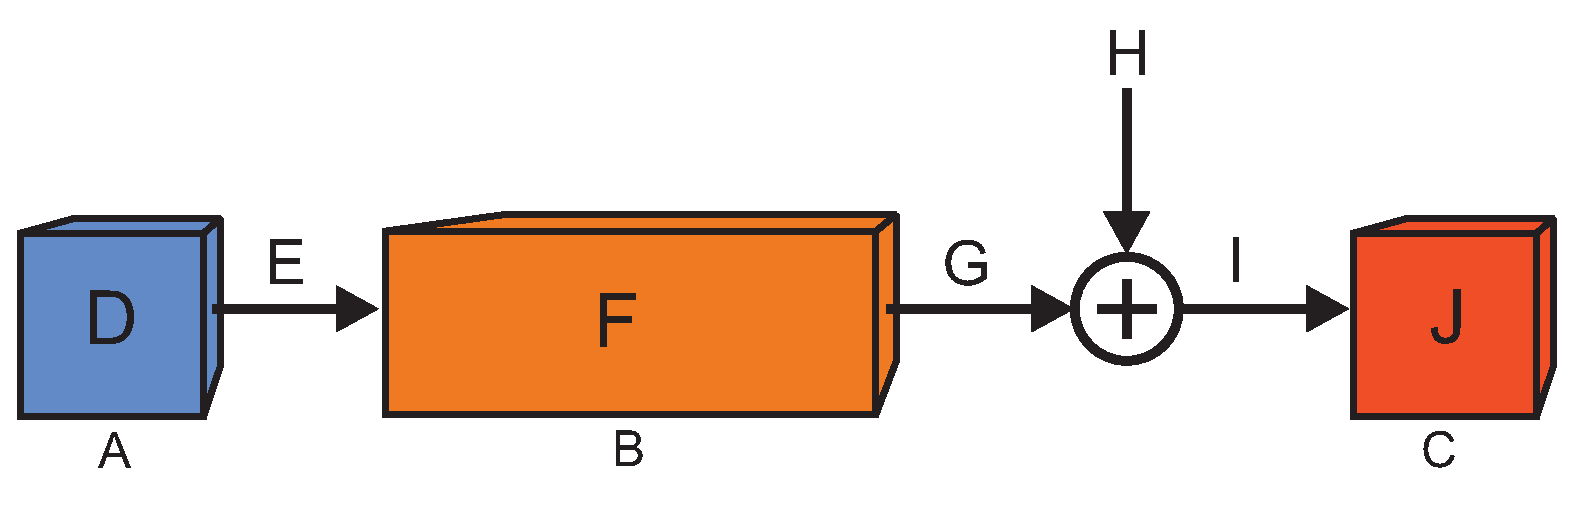
\includegraphics[width=0.49\textwidth]{images/PLCchannel.eps}
	\caption{The block diagram of a PLC system.}
	\label{PLCchannel}
\end{figure}

Fig. \ref{Hybchannel} shows the block diagram that result from the use of the hybridism concept in a data communication system, in which \ac{PLC} and \ac{WLC} channels are employed in cascade without an intermediate data communication node between them. As this figure shows, \ac{PLC} devices are connected to electric power grids through a coupling circuit while the \ac{WLC} devices are connected to the air through an antenna. Both devices directly communicate with each other because they operate in the same frequency band. The received signals at the input of the hybrid \ac{PLC}-\ac{WLC} channels, which is supposed to be a linear time-varying system, are expressed as
\begin{equation} \label{received signal2}
Y_{PW}(t) = \int_{-\infty}^{+\infty} h_{PW}(t,\tau) X(\tau) d\tau + V_{PW}(t),
\end{equation}
for the signal propagation from the \ac{PLC} device to the \ac{WLC} device (i.e., \ac{PLC}~$\rightarrow$~\ac{WLC} direction), and
\begin{equation} \label{received signal3}
Y_{WP}(t) = \int_{-\infty}^{+\infty} h_{WP}(t,\tau) X(\tau) d\tau + V_{WP}(t),
\end{equation}
for the reverse path, which is defined by the signal propagation from the \ac{WLC} device to the \ac{PLC} device (i.e., \ac{WLC}~$\rightarrow$~\ac{PLC} direction). In (\ref{received signal2})-(\ref{received signal3}),  $X(t)\in \mathbb{R}$ is the transmitted signal modeled as a wide sense stationary stochastic process; $h_{PW}(t,\tau)\in \mathbb{R}$ and $h_{WP}(t,\tau)\in \mathbb{R}$ denote the \acp{CIR} when an impulse at the instant $\tau$ is applied to the channel defined by the \ac{PLC}~$\rightarrow$~\ac{WLC} and \ac{WLC}~$\rightarrow$~\ac{PLC} directions, respectively; $V_{PW}(t)\in \mathbb{R}$ and $V_{WP}(t)\in \mathbb{R}$ are, respectively, the \ac{WLC} and \ac{PLC} additive noise components, modeled as two different wide sense stationary random processes found at the input of the receivers, when the \ac{PLC}~$\rightarrow$~\ac{WLC} and \ac{WLC}~$\rightarrow$~\ac{PLC} directions take place; $Y_{PW}(t)\in \mathbb{R}$ and ${Y}_{WP}(t)\in \mathbb{R}$ are wide sense stationary random processes denoting the received signals, respectively, in the \ac{PLC}~$\rightarrow$~\ac{WLC} and \ac{WLC}~$\rightarrow$~\ac{PLC} directions.

\begin{figure}[h]
	\centering
	\psfrag{A}[c][c][0.9]{Wall}
	\psfrag{B}[c][c][0.9]{hybrid-PLC}
	\psfrag{C}[c][c][0.9]{Transceiver}
	\psfrag{D}[c][c][0.9]{PLC coupler}
	\psfrag{E}[c][c][0.9]{Power}
	\psfrag{F}[c][c][0.9]{line}
	\psfrag{G}[c][c][0.9]{PLC signal}
	\psfrag{H}[c][c][0.9]{hybrid-Wireless}
	\psfrag{I}[c][c][0.9]{Transceiver}
	\psfrag{J}[c][l][0.9]{Antenna}
	\psfrag{K}[c][c][0.9]{Wireless$~~~~~~~~~~~~~~~~~~$}
	\psfrag{L}[c][c][0.9]{signal$~~~~~~~~~~~~~~~~~$}
	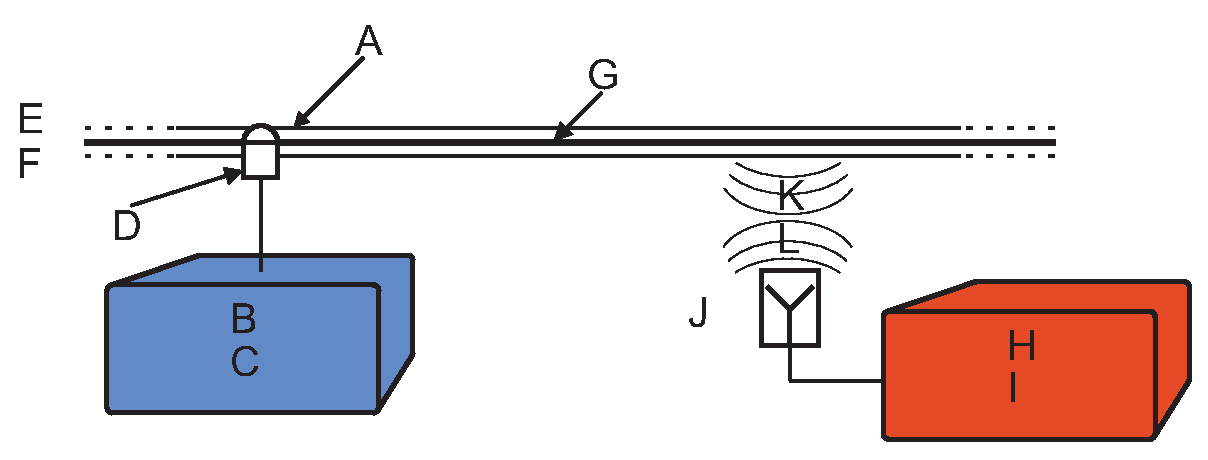
\includegraphics[width=0.49\textwidth]{images/Hybrid_channel.eps}
	\caption{The block diagram of a hybrid PLC-WLC system.}
	\label{Hybchannel}
\end{figure}

It is important to highlight that the symmetry of the hybrid \ac{PLC}-\ac{WLC} \ac{CFR} is verified when the transmitter and the receiver have the same access impedance \cite{thiago:hyb}. Mathematically, $h_{PW}(t,\tau)=h_{WP}(t,\tau)$ agrees with the results presented in \cite{Galli:indoor}, which focuses only on \ac{PLC} channels. Due to the specific characteristics of each media (e.g., power line and air), the symmetry property does not hold true for the additive noises $V_{PW}(t)$ and $V_{WP}(t)$ \cite{thiago:hyb}. 

Given back to \ac{PLC} systems, it is important to emphasize that the random \ac{LPTV} behavior of \ac{PLC} channels, $h_P(t,\tau)$, is considered to be a cyclostationary stochastic random process with a period equal to a half of the mains frequency \cite{Colen:TCRA}. Based on the knowledge of the coherence time, $T_c \in \mathbb{R}_+$, of the \ac{PLC} channels, the mains cycle ($50$~Hz or $60$~Hz) can be divided into microslots of time interval duration equal to $T_m\in \mathbb{R}_+|T_m < T_c$ and, as a consequence, the \ac{PLC} channels can be modeled as \ac{LTI} during the time interval duration of one microslot \cite{Colen2016}. In other words, the \ac{CIR} of a \ac{PLC} channel during the $i^{th}$ microslot can be expressed as
\begin{equation} \label{discreteh}
h_{P,i}(t),~\forall~t \in [iT_{m}, (i+1)T_{m}] \mid T_{m} \le T_{c}.
\end{equation}
Similar to \ac{PLC} systems, the hybrid \ac{PLC}-\ac{WLC} systems operates in the baseband. Therefore, the aforementioned mathematical formulation will also take place to the \acp{CIR} of the hybrid \ac{PLC}-\ac{WLC} channels bearing in mind that the \ac{PLC} component of these channels exert an influence on the behavior of them. Therefore, the following discussion applies to both treated in-home channels.

From now on, we drop the index $i$ for the sake of simplicity. Based on this assumption, the discrete-time representation of the \ac{CIR} of the \ac{PLC} channel in a single microslot is given by
\begin{equation} \label{discreteCFR}
h[n] = h_{a}(t)|_{t=nT_s} , n = 0,1, \ldots, L_h-1, 
\end{equation}
where $a\in \{P, WP, PW \}$, $L_{h}$ is the length of the $a^{th}$ \ac{LTI} channel, $T_s=1/f_s$ is the sampling period and $f_s=2B$~Hz is the sampling frequency. Usually, the value of $L_{h}$ impact the specification of the \ac{HS-OFDM} scheme, which is supposed to operate in the baseband. As a result, the length of the an \ac{HS-OFDM} symbol is ($2N$) and $L_{cp} \gg L_h$, in which $L_{cp}$ stands for the length of cyclic prefix. Moreover, $B/N \le B_{c,a}$, in which $B_{c,a}$ is the coherence bandwidth of the $a^{th}$ channel. In order to work with $N$ subcarriers in the \ac{HS-OFDM} scheme for performing \ac{CFR} estimation, the zero padding has to be applied to $\{h[n]\}$. In vectorial terms, ${\bf h}=[h_0 h_1 \ldots h_{L_h-1}]^T$ is such that $h_n=h[n]$. Then the vectorial representation of the \ac{CFR} associated with the extended version of $\mathbf{h}$ is expressed as
\begin{equation}
\mathbf{H} = \mathbf{W}_{2N}  \begin{bmatrix} \mathbf{I}_{L_h} \\ \mathbf{0}_{(2N-L_{cp})\times L_{h}} \end{bmatrix} \mathbf{h},
\end{equation}
where $\mathbf{W}_{2N} \in \mathbb{C}^{2N\times 2N}$ denotes the $2N \times 2N$-size \ac{DFT} matrix, $ \mathbf{I}_{L_h} \in \mathbb{R}^{L_h\times L_h}$ denotes an $L_h\times L_h$-size identity matrix, and $ \mathbf{0}_{(2N-L_{cp})\times L_{h}} $ is an $ (2N-L_{cp})\times L_{h}$ null matrix. The $k^{th}$ element of the vector $\mathbf{H}=[H_0 H_1 \ldots H_{2N-1}]^T \in \mathbb{C}^{2N\times 1}$ may be expressed in the polar form as $H_k=|H_k|\exp(j \Theta_k)$, in which $|.|$ denotes the absolute value and $\Theta_k$ is the phase of $H_k$. Since the \ac{CIR} of the $a^{th}$ channel is real-valued, it means that \ac{CFR} posses the hermitian symmetry property and, as a consequence, the first half of samples of the \ac{CFR} are sufficient for representing the whole $a^{th}$ channel. We assume that the vectors $|{\bf H}|\triangleq [|H_0||H_1|\ldots |H_{N-1}|]^T$ and ${\bf \Theta}\triangleq[\Theta_0\Theta_1\ldots \Theta_{N-1}]^T$ define two distinct random processes that represent, respectively, the magnitude and phase of the first half of the vector $\mathbf{H}$. It is important to emphasize that the nature of the $a^{th}$ channel indicates that the vectors $|{\bf H}|$ and ${\bf \Theta}$ are non-stationary and correlated random processes. 

%Since it is well known that the \ac{CFR} phase component can be modeled as an uniform distribution \cite{unif_phase}, 
From now on, we will focus only on the magnitude of \ac{CFR} magnitude because it is useful for data communication purposes once its knowledge and of the squared magnitude (i.e.,  $|{\bf H}|^2\triangleq[|H_0|^2|H_1|^2\ldots |H_{N-1}|^2]^T$) of the \ac{CFR} allows to derive closed-form expression of theoretical channel capacity, physical layer security, and other important information of the channel. Also, the most important thing, there is a lack a consensus in terms of its modeling. 

In this regard, let us assume that the $k^{th}$ \ac{r.va.} belonging to the magnitude random processes (i.e., the element $|H_k|$) is modeled by an statistical distribution owing a set of parameters represented by $\mathcal{C}_{|H|_k} = \{ \alpha_{1}[k], \cdots, \alpha_{U}[k] \}$, which is constituted by $U \in \mathbb{N}_+$ parameters. Note that $\alpha_{u}[k] \in \mathbb{R}$ is the $u^{th}$ parameter associated with the chosen statistical distribution offering the best description of the $k^{th}$ element of the vector $|{\bf H}|$.

Given the aforementioned formulation, the following research questions arise: \textit{What kind of statistical distributions are suitable for modeling the random variables that constitute the vector $|{\bf H}|$? Could we state that $|{\bf H}|$ is a stationary random process?} The following sections try to answer these challenging research questions.

\section{Statistical Modeling Methodology}

With the purpose of addressing the research questions posed in the previous section and introducing the models of \ac{CFR} magnitudes related to \ac{PLC} and hybrid \ac{PLC}-\ac{WLC} channels, an enhanced statistical modeling method, which is based on the one introduced in \cite{Luis:AI}, is devised through the top-down approach. Basically, each element of the \ac{r.v.} ${\bf |H|}$ is assumed to be uncorrelated. This is an interesting approach to come up with simple statistical models of ${\bf |H|}$.

The statistical modeling can be summarized in searching for the statistical distributions offering the best fits to a data set obtained from a measuring campaign (i.e., measured \ac{CFR} estimates). It means that the type of statistical distribution together with its parameters are the modeling information for each element of the \ac{r.v.}  ${\bf |H|}$. In other words, the model is the chosen statistical distribution together with its parameters.

In addition, it is important to come up with the statistical model of parameters of $|H(e^{j\omega})|$, which is the discrete-time Fourier transform of $h(t)$. To do so, a technique capable of yielding a suitable interpolation with a reduced number of parameters and without presenting edge effects, such as that ones reported in \cite{Luis:AI} is a very convenient solution. In fact, standard interpolation technique may demands a large number of parameters \cite{mitra} once all elements of the vector of parameters are used for the interpolation purpose. %Based on the fact that we are yielding statistical distributions for the elements of the \ac{r.v.} $\bf |H|$, the interpolation technique is applied to the set of parameters of the statistical distribution modeling each element of the \ac{r.v.} $\bf |H|$.

Regarding the chosen statistical distribution, we can assume that $\alpha_u (\omega) = F_u(\omega; \alpha_{u}[0], \cdots, \alpha_{u}[N-1])$, in which $\omega \in [0,2\pi)$, is such that $\alpha_{u}[k] = F_u(2\pi k/N; \alpha_{u}[0], \cdots, \alpha_{u}[N-1]),u=1,\cdots,U$. In this context, the problem of interpolation consists of finding an approximation $P_u(\omega)$ for the function $F_u(\omega)$ within the defined class of functions, in the way that it can obtain the same values at the points $\omega_k = 2\pi k/N$ (i.e., $F_u(\omega_k)=P_u(\omega_k)$). The Lagrange Interpolation is the direct solution to obtain $P_u(\omega)$; however, the degree of interpolating Lagrange polynomial is strictly related to the amount of points (nodes)  $\omega_k = 2\pi k/N$, which makes the problems with high number of input data difficult to solve. The use of Splines can mitigate this problem once it divides the interval into $L$ subintervals, constructs the interpolating polynomial $P_{u,l}(\omega),l=1,\cdots,L$, in the $l^{th}$ subinterval separately and groups the resulting interpolation polynomials to obtain $P_u(\omega)$. Another advantage of Splines is their capacity of avoiding the Runge's phenomenon. This contribution applies the cubic Splines \cite{Spline} due to their characteristics of not needing to use uniform intervals of interpolation, producing smoother curves, interpolating the bounds of the intervals and generating a continuous curve over the chosen frequency subband. 

Based on the aforementioned discussion, the proposed enhanced statistical modeling method can be organized in four steps. Essentially, it consists on trying several statistical distributions to model each element of the \ac{r.v.} $\bf |H|$, choosing the best statistical distribution by adopting well-established criteria and performing the approximation of the function by using the Splines-based interpolation technique. The following steps implement the proposed method:
\begin{itemize}
	\item \textbf{Step \#1}: Model all elements of the \ac{r.v.} $\bf |H|$ with the set of statistical distributions that addressed the characteristics of its elements. It is important to highlight that ${\bf |H|} \in \mathbb{R}_{+}^{N\times 1}|0 \leq {|H_k|} \leq 1$ determines the suitability of a set of statistical distributions for modeling the magnitude component.
	\item \textbf{Step \#2}: Appraise the set of statistical distributions, for each element of the \ac{r.v.} $\bf |H|$ in order to select the best statistical distribution. In this sense, consider the majority vote rule \cite{vote} over four chosen criteria (\ac{MLE}, \ac{AIC}, \ac{BIC}, and \ac{EDC} information criteria \cite{Dorea:Sim}, \cite{Cabral:Multi}, \cite{Andrei:Meas}). By considering the \ac{MLE} criterion, the best statistical modeling is the distribution that achieves the maximum value, whereas for the \ac{AIC}, \ac{BIC}, and \ac{EDC} information criteria, the best modeling is the statistical distribution that achieves minimum values. 
	In order to visualize when an statistical distribution yields the best results in terms of a \ac{MLE} criterion, a kind of the log-likelihood ratio, which in our case is expressed as
    \begin{equation}
    \rho_{A} [k] \triangleq \dfrac{\underset{\mathcal{A}}{\max} \,\, \, MLE[k]}{MLE[A,k]},
    \label{eq:log-lik}
    \end{equation}
    is adopted. Note that $ MLE[A,k]$ is the value of the log-likelihood associated with one of the chosen statistical distributions, which is denoted by $A$, belonging to the set of statistical distributions $\mathcal{A}$ for the $k^{th}$ frequency tone. Also, $\underset{\mathcal{A}}{\max} \,\, \, MLE[k]$ is the value of the log-likelihood related to the statistical distribution yielding the best statistical model. The best results are achieved when $\rho_A [k] \rightarrow 1$. Note that $\rho_A [k] \rightleftharpoons \rho_A (\omega) \rightleftharpoons \rho_A (f)$.
	\item \textbf{Step \#3}: Find the statistical distribution yielding the best statistical modeling for the largest number of elements of the \ac{r.v.} $\bf |H|$. It is important to note that the said distribution must achieve a minimum percentage ratio over the best results yielded by (\ref{eq:log-lik}), for the elements in which the distribution is not the best model, to be considered a valid model over the desired frequency band. This statistical distribution is chosen as the statistical distribution for all elements of the \ac{r.v.} $\bf |H|$. As a results, the set of parameters associated with the statistical distribution is given by $\{\alpha_{1}[0], \cdots, \alpha_{1}[N-1]$,   $\cdots, \alpha_{U}[0], \cdots, \alpha_{U}[N-1]\}$.
%Finally, the set of parameters (i.e., $\mathcal{C}_{|H|_k} = \{ \zeta_{1}[k], \cdots, \zeta_{U}[k] \}$ ) associated with the chosen statistical distributions for each element of the \ac{r.v.} $\bf |H|$ is obtained.
    \item \textbf{Step \#4}: Interpolate the parameters using the cubic Spline interpolation for obtaining $\alpha_u (\omega) = F_u(\omega; \alpha_{u}[0], \cdots, \alpha_{u}[N-1]), u=1,\cdots,U$. This procedure consists on dividing the desired frequency band into $L$ subbands delimited by $\omega_{l,\textnormal{lower}}$ and $\omega_{l,\textnormal{upper}}$ bounds, and evaluating a third-degree polynomial that describes the $l^{th}$ subband. Note that all subbands address $\omega \in [0,2\pi)$ and the coefficients of the $l^{th}$ polynomial are obtained for each subband following the procedure discussed in \cite{ENA,CS1}.      
\end{itemize}


\section{Numerical Results}

The statistical analyses were carried out by means of two data sets constituted by \ac{CFR} estimates of in-home \ac{PLC} and in-home hybrid \ac{PLC}-\ac{WLC} channels, which cover the frequency band between $1.7$ and $100$~MHz. These data set were acquired through a measurement campaign, detailed in \cite{Thiago:Characterization,thiago:hyb}. Regarding the \ac{PLC} portion of the measurement campaign, a total of $245$ different combinations of outlets pairs were measured, allowing the acquisition of $148,037$ different \ac{CFR} estimates, with approximately $604$ consecutive \ac{CFR} estimates for each individual measure. Considering the hybrid \ac{PLC}-\ac{WLC} portion of the measurement campaign, $293$ different combinations of locations for both hybrid-\ac{PLC} and hybrid-\ac{WLC} transceivers were evaluated. As a result, a total of $175,428$ different \ac{CFR} estimates were acquired, with approximately $600$ consecutive \ac{CFR} estimates for each individual channel acquisition. Two different cases were considered during this scenario, named \textit{short-path channel} and \textit{long-path} channel, respectively. Regarding the \textit{short-path} channel, the \ac{WLC} transceiver was randomly positioned within a $2$~m radius circle centered at the outlet in which the \ac{PLC} transceiver was connected, this scenario was responsible for estimating around $136,683$ \acp{CFR} in $200$ different combinations of locations for both \ac{PLC} and \ac{WLC} transceivers. On the other hand, in the \textit{long-path} channel scenario, the \ac{WLC} transceiver was randomly placed into an area defined as a swept circle, having an outer and inner radius of $6$~m and $2$~m, respectively, centered in the outlet in which the \ac{PLC} transceiver was connected. This case allowed to obtain $38,745$ \ac{CFR} estimates in $93$ different combinations of locations for both \ac{PLC} and \ac{WLC} transceivers.

The methodology applied to obtain the \ac{CFR} estimate was the one discussed in \cite{Thiago:FR}. It relies on a measurement setup and the use of an \ac{HS-OFDM} scheme \cite{HSOFDM,Picorone}. The measurement setup covers signal generation and acquisition boards, rugged computers, and coupling devices \cite{Luis:AI,Coupling:PLC}, while the \ac{HS-OFDM} scheme is a kind of sounding technique for estimating \ac{CFR} in the discrete time-domain when the data communication channel is in the baseband. After applying the aforementioned techniques, the average of $L_1\in \mathbb{N}_+, L_2\in \mathbb{N}_+, L_3\in \mathbb{N}_+ $ consecutive \ac{CFR} estimates are obtained and then stored as a valid \ac{CFR} estimate for the \ac{PLC}, \ac{PLC}-\ac{WLC} \textit{short-path} and \ac{PLC}-\ac{WLC} \textit{long-path} channels respectively, respecting the coherence time of the mentioned channels. This last procedure is applied aiming to reduce the impulsive noise influence on the \ac{CFR} estimates.

It is important to emphasize that one \ac{CFR} estimate is obtained during a time interval corresponding to one \ac{HS-OFDM} symbol period $(T_{\textrm{sym}})$ duration and, as a consequence, it assumes that the time interval duration of the \ac{HS-OFDM} symbol must be shorter than the coherence time of the \ac{PLC} or \ac{PLC}-\ac{WLC} channel. Based on the set of parameters of the estimation technique, an enhanced channel estimate is obtained every $T_{\textrm{sym}}=(2N + L_{cp}) T_s = 23.04$~$\mu$s, where $N=2048$ is the number of \ac{BPSK} modulated subcarriers of the \ac{HS-OFDM} symbol, $L_{cp}=512$~samples is the length of the so-called \ac{CP}, $f_s=200$~MHz is the sampling rate and $T_s=1/f_s=5$~ns is the sampling period. According to \cite{Canete:AIPLC}, $600~\mu$s is the minimum time period within which the in-home \ac{PLC} channel can be considered time invariant in Spain, while \cite{Thiago:Characterization} pointed out $950~\mu$s for the Brazilian in-home \ac{PLC} channels. In addition, \cite{thiago:hyb} showed that  $156~\mu$s and $39.5~\mu$s are the minimum time period within which the in-home hybrid \ac{PLC}-\ac{WLC} \textit{short-path} and \textit{long-path} channels, respectively, can be considered time invariant.

Moreover, the assumed value of $N$ and the chosen frequency band ($1.7-100$)~MHz, results in \ac{CFR} estimates with a corresponding frequency resolution of $\Delta f=48.83$~kHz, which is shorter than the coherence bandwidth of Brazilian and Spanish in-home PLC channels \cite{Canete:AIPLC,Thiago:Characterization} as well as shorter than the coherence bandwidth of Brazilian in-home hybrid \ac{PLC}-\ac{WLC} channels \cite{thiago:hyb}. Being shorter than the coherence bandwidth means that each sample of a valid \ac{CFR} estimates is representative for carrying out the statistical analyses. Furthermore, for sake of clearness, all numerical results are presented in the continuous-time domain rather than the discrete-time one.

In order to perform the statistical analyses of the valid \ac{CFR} magnitudes, the following statistical distributions were adopted: Beta, Birnbaum-Saunders, Gamma, Logistic, Log-normal, Normal, Rayleigh, Rician, t Location-Scale, and Uniform. These statistical distributions cover the well-established ones in the telecommunication field and those applied to model a random variable belonging to $\mathbb{R}_+$.

\subsection{In-home PLC channels}\label{sec:MMPLC}

For illustrative purpose, Fig. \ref{respfreq} portrays five valid estimates of the \ac{CFR} magnitude, considering the aforementioned frequency band. Each valid \ac{CFR} estimate was obtained by averaging  $L_1 = 10$ consecutive \ac{CFR} estimates of a \ac{PLC} channel associated with an in-home electric power circuit, which was measured during the measurement campaign. Note that the channel attenuation ranges from approximately $-30$~dB up to $0$~dB. These plots show that the in-home \ac{PLC} channels present a small time-varying behavior during a time interval shorter than $1$~ms once each valid \ac{CFR} estimate covers a time interval equal to $\Delta T = L_1 T_{\textrm{sym}} \approx 230.4\,\mu$s and, as a consequence, $5\Delta T = 1.15$~ms. In other words, the coherence time in an in-home Brazilian PLC channel is larger than in Europe and US, as detailed in \cite{Thiago:Characterization}.

\begin{figure}[h]
	\centering
	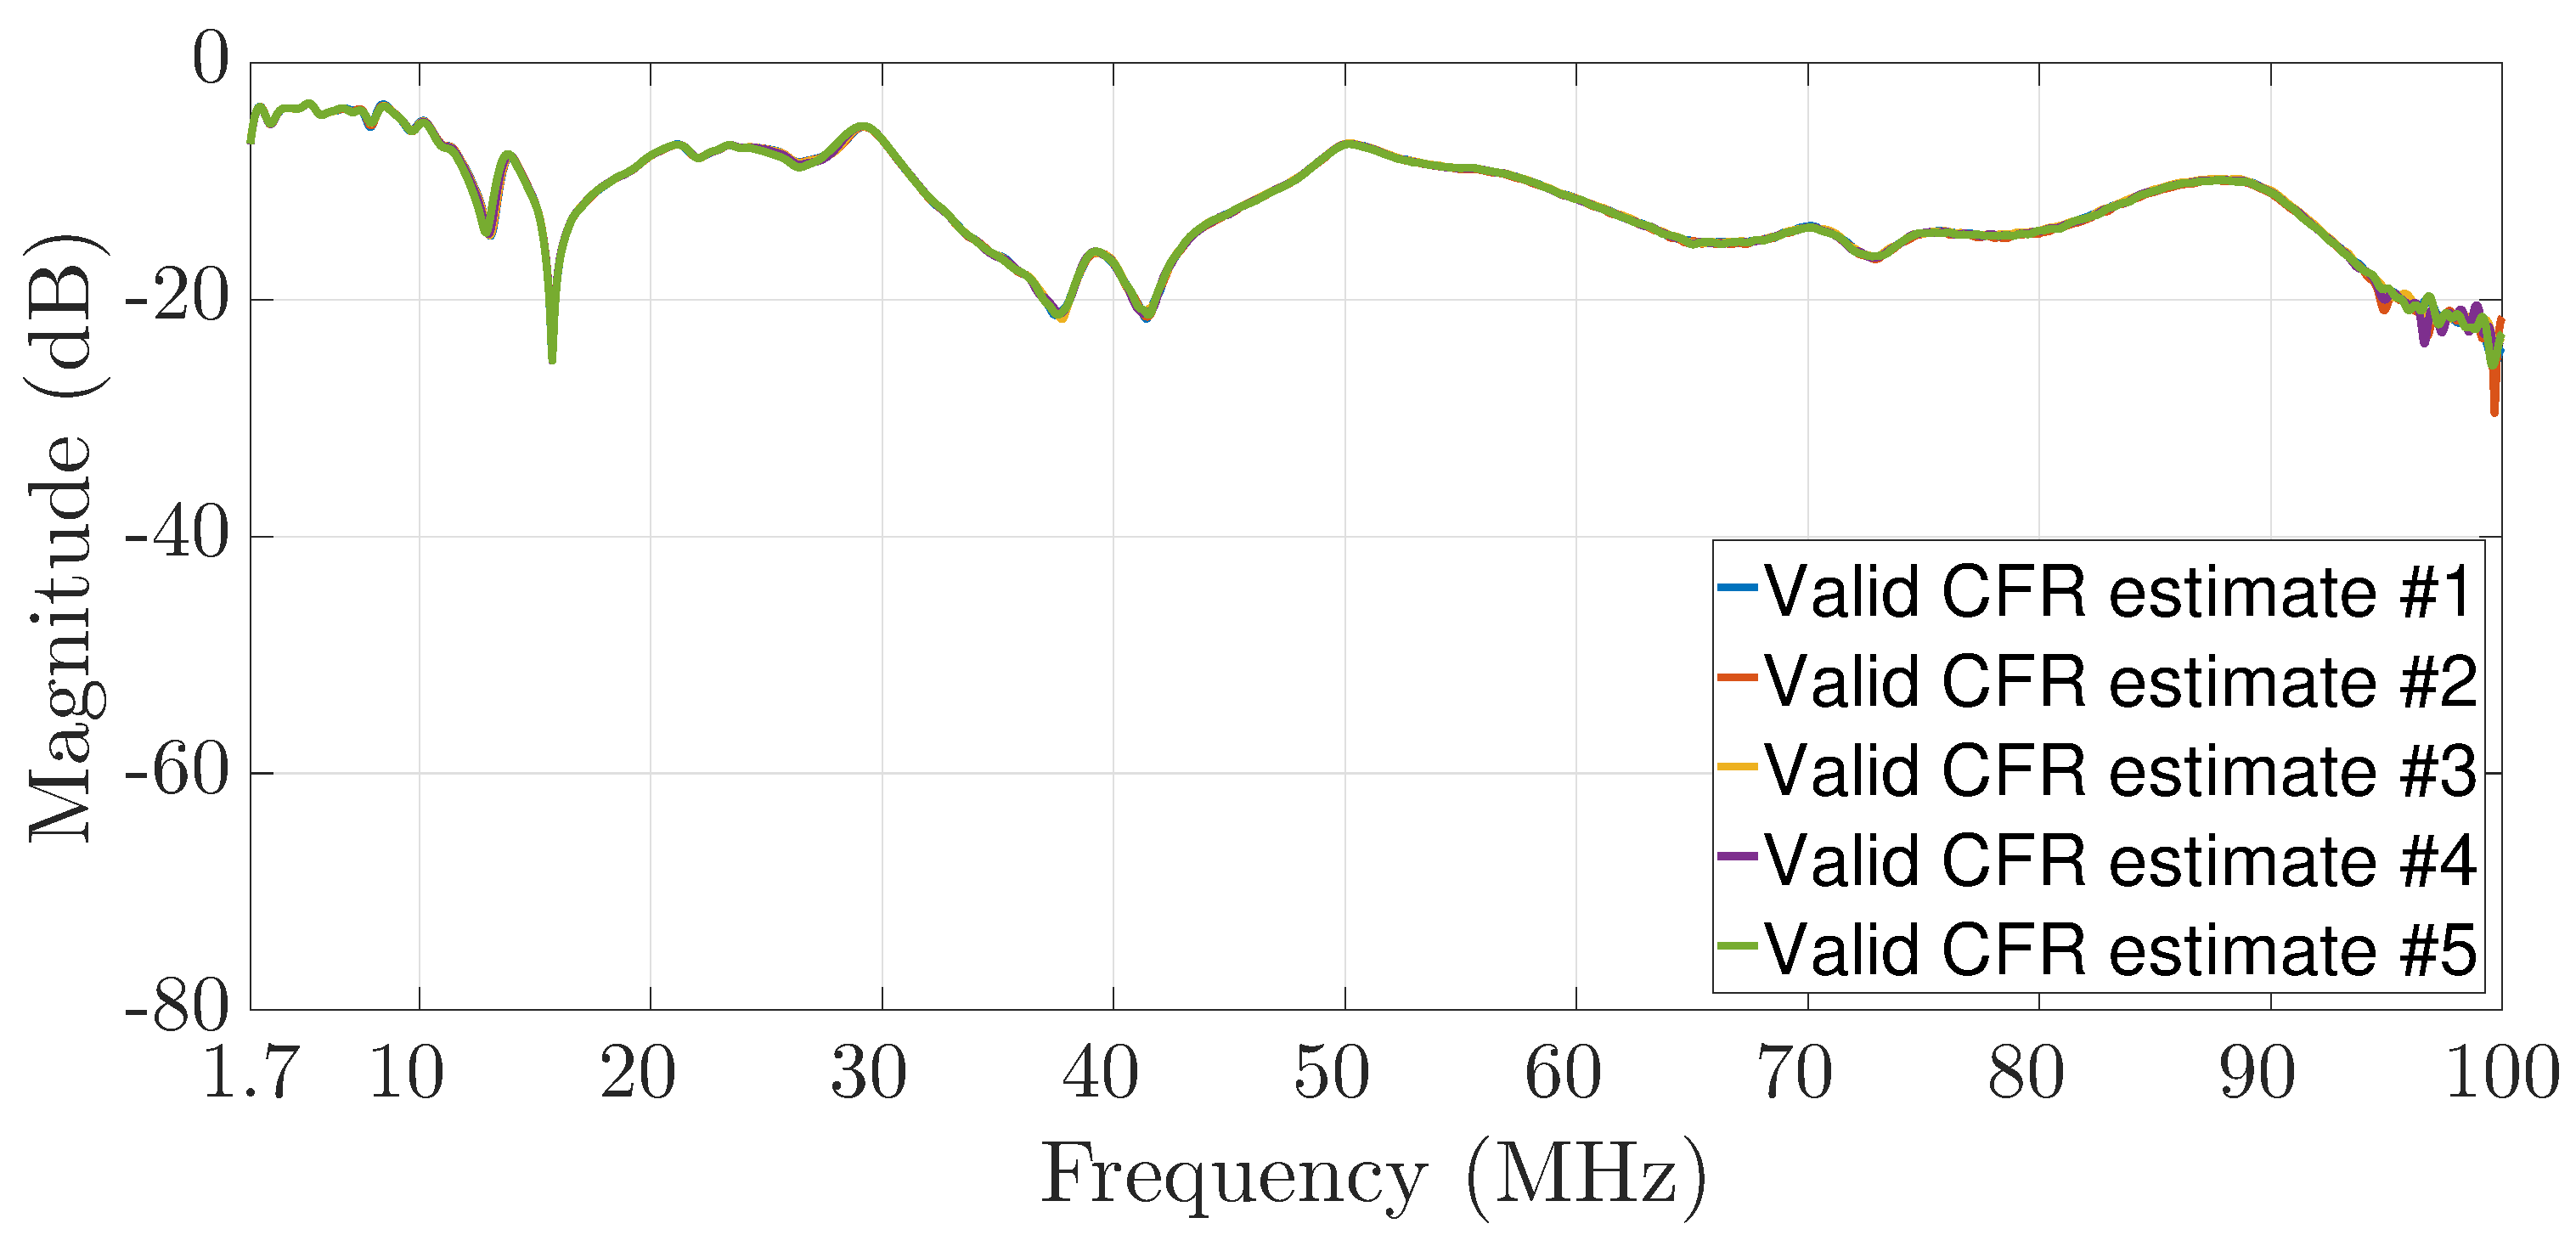
\includegraphics[width=0.49\textwidth]{images/respfreq_1.7.eps}
	\caption{Five consecutive and valid \ac{CFR} Magnitudes of the measured in-home \ac{PLC} channel.}
	\label{respfreq}
\end{figure}

Fig. \ref{MAG_percent} shows the relative frequency of statistical distributions that had modeled, in accord with the adopted criterion, the magnitude of the whole set of valid \ac{CFR} estimates. It is noted that there is not only a single distribution that models the majority of the magnitudes, but three different statistical distributions stand out as possible candidates to model the \ac{CFR} magnitudes. As a matter of fact, in 35\% of the \ac{CFR} estimates data set the Beta distribution resulted in the best model, in 30\% of it  the Birnbaum-Saunders distribution offered the best modeling and in 24\% of it the Log-normal distribution yielded the best modeling. 

\begin{figure}[h!]
	\centering
	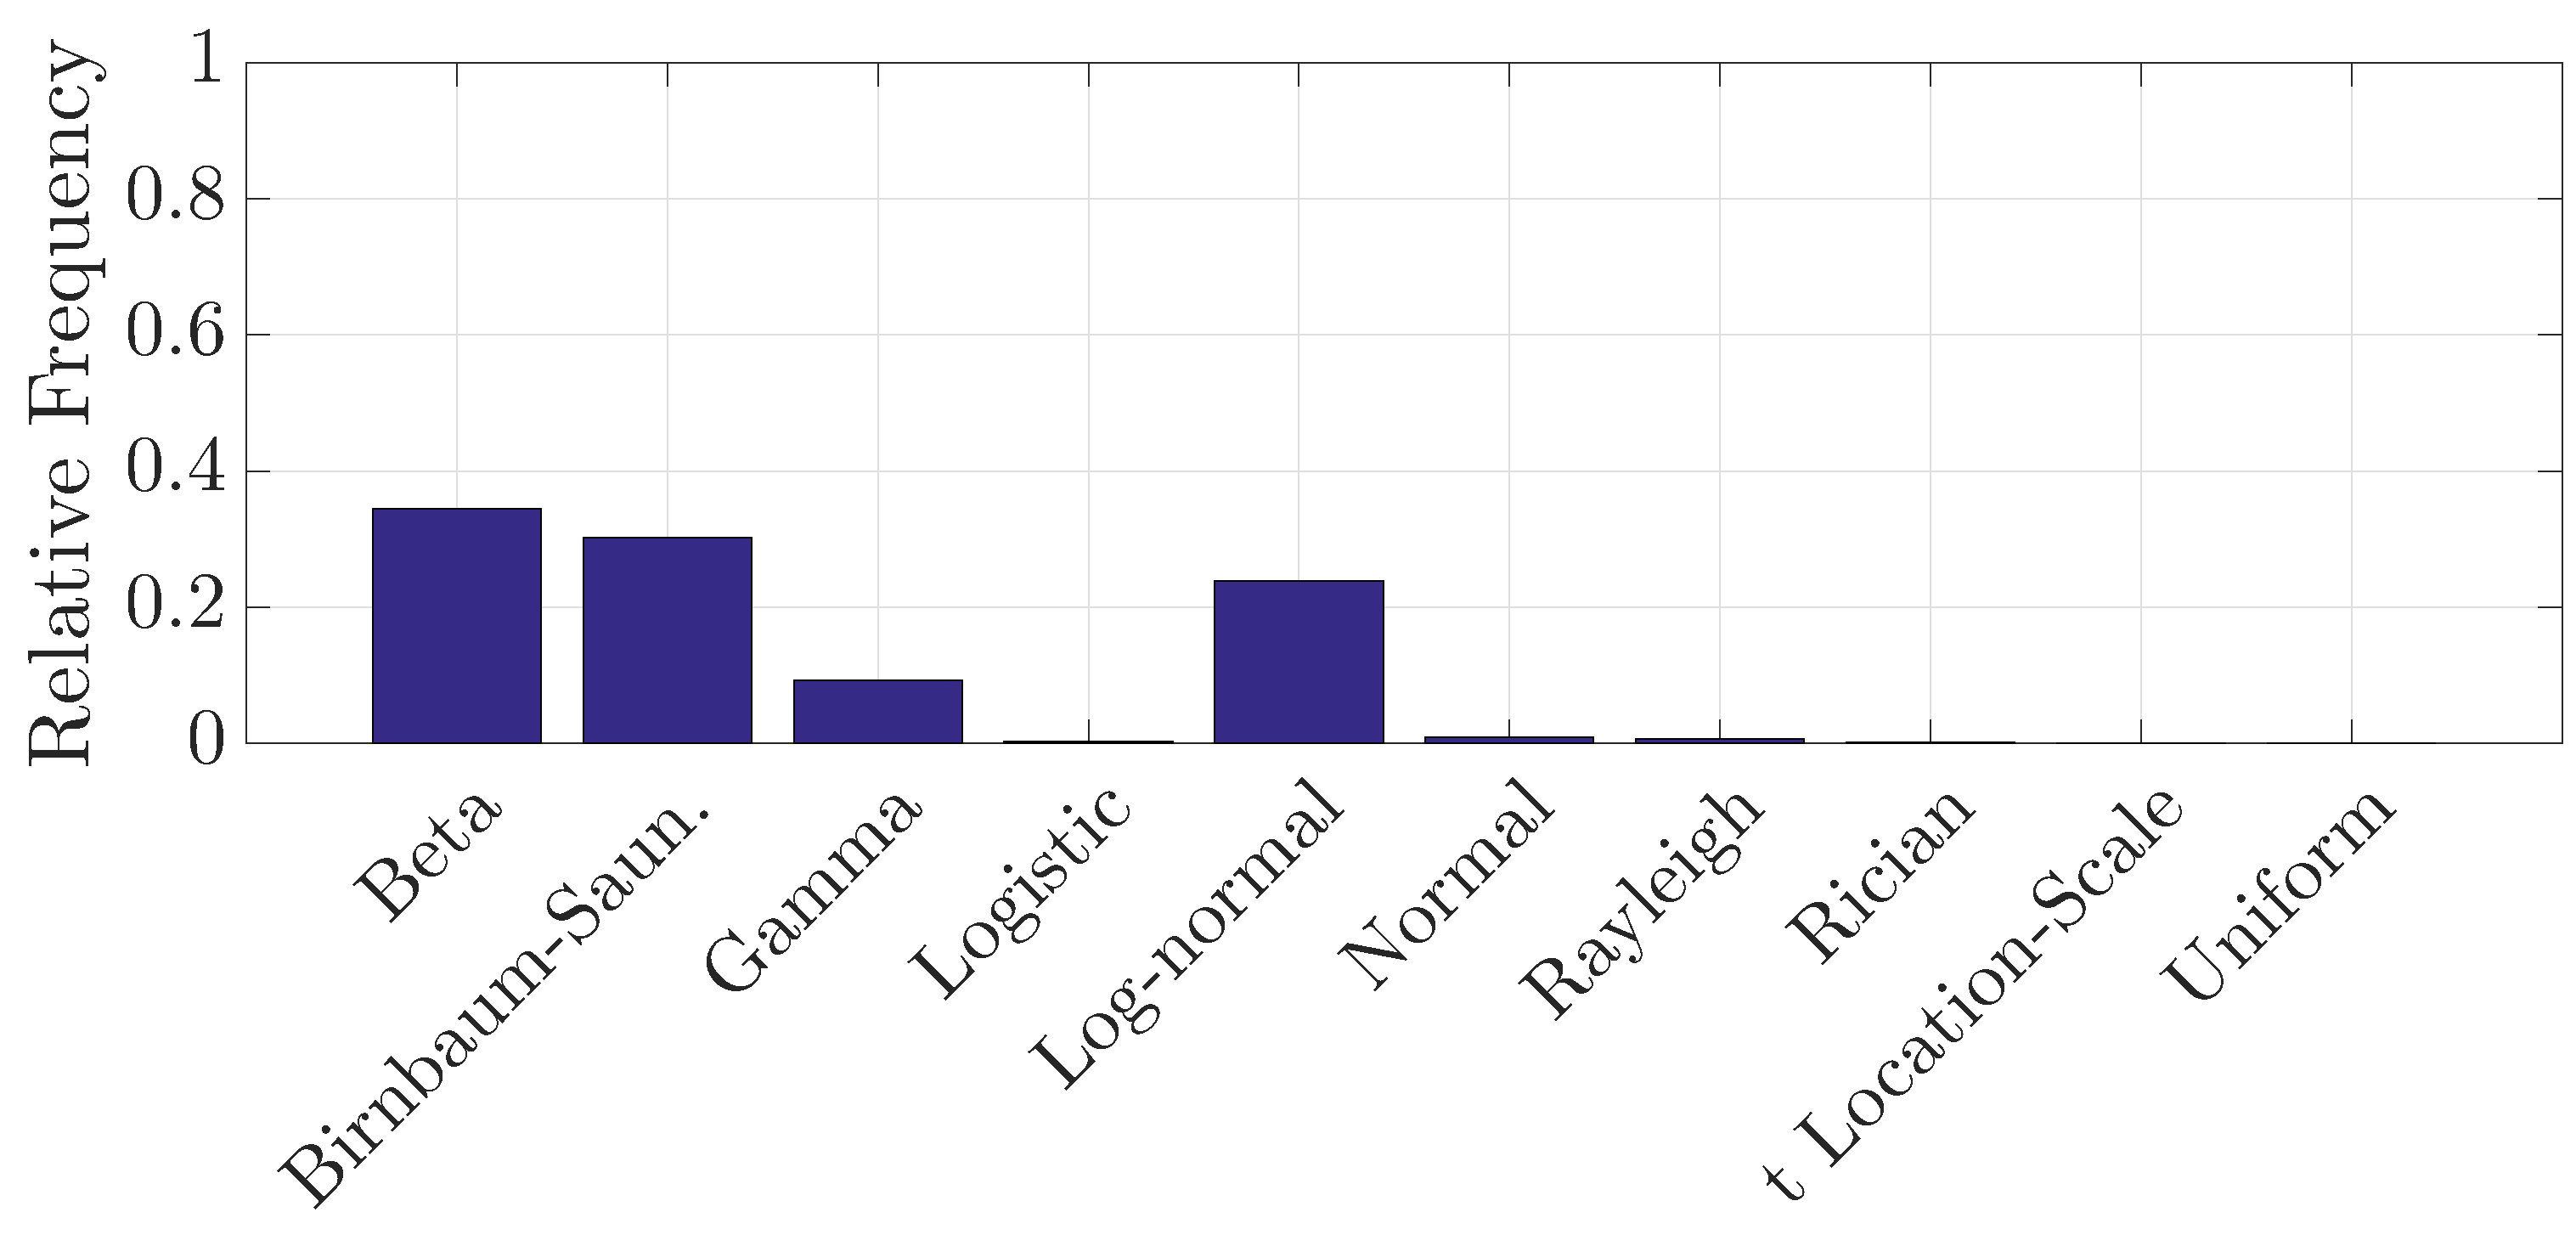
\includegraphics[width=0.49\textwidth]{images/Mag_percent.eps}
	\caption{The relative frequency associated with the chosen statistical distribution that best models the \ac{CFR} magnitude in accord with the adopted criteria.}
	\label{MAG_percent}
\end{figure}

In order to evaluate which of the three distributions is the best choice to model the magnitude component of the \ac{CFR} estimates, we use (\ref{eq:log-lik}). Fig. \ref{fig:Log_like} shows the values of $\rho_{A}(f)$ for the three best statistical distributions candidates to model the magnitude of the valid \ac{CFR} estimates. The threshold value $1.2$, corresponding to a deviation of $20\%$ from the best achievable result, was heuristically chosen as the upper bound, indicated by a red dashed line, under which the statistical distribution can be considered good enough to model the \ac{CFR} of in-home \ac{PLC} channels. Note that the vertical axis was limited to the range from $0$ up to $5.0$ to facilitate the visualization and the comparison among the $\rho_{A} (f)$ curves. These curves emphasize the suitability of the Beta distribution to model the samples of the magnitude of the valid \ac{CFR} estimates. Overall, the results presented in Fig. \ref{MAG_percent} and Fig. \ref{fig:Log_like} strongly support the use of the Beta distribution to model the magnitude of the valid \ac{CFR} estimates of the measured in-home Brazilian \ac{PLC} channels. This result is different from previous works that had suggested the Log-normal or Rayleigh distributions to model this magnitude, see \cite{Galli:Wireline,RayleighPLC}.

\begin{figure}[h!]
	\centering
	\psfrag{AAA}[c][c][0.8]{$\rho_{A} (f)$}
	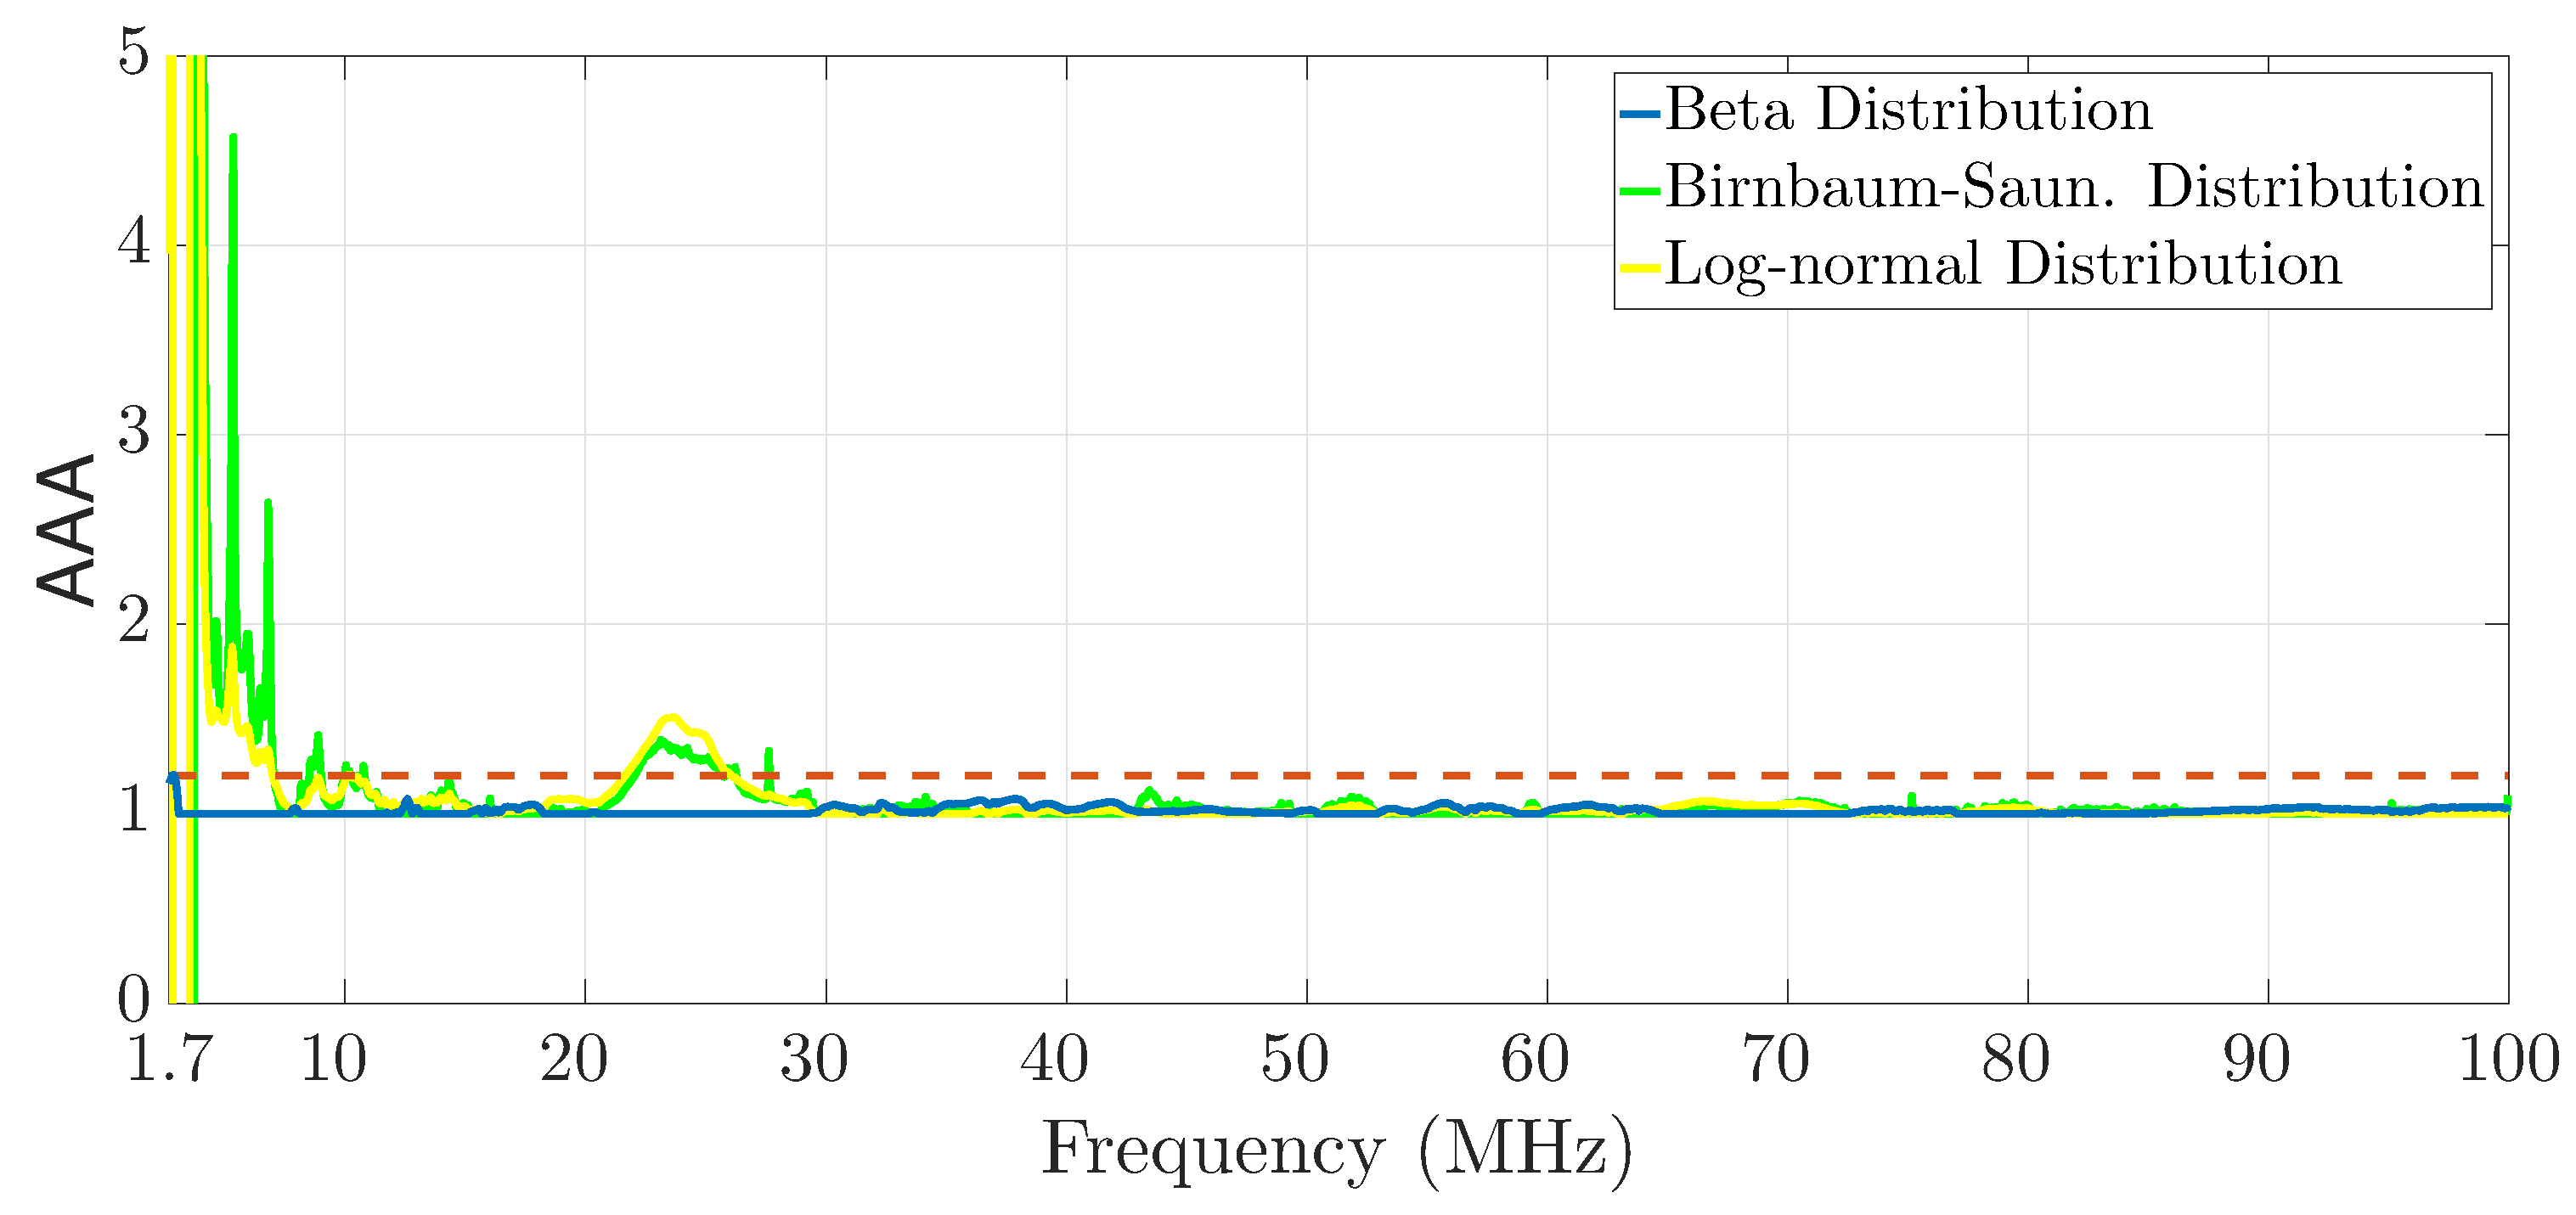
\includegraphics[width=0.5\textwidth]{images/LLH_BETA_BIRN_LogN_1.7.eps}
	\caption{The values of $\rho_{A} (f)$ for the Beta, Birnbaun-Saunders and Log-normal distributions.}
	\label{fig:Log_like}
\end{figure}

Based on the aforementioned discussion, we can model the magnitude of the valid \ac{CFR} estimates by using only one statistical distribution (i.e., the Beta distribution). However, the statistical analysis of the magnitude of the valid \ac{CFR} estimates shows that each sample of it must be modeled with a set of parameters of the Beta distribution assuming different values. If $\mathcal{C}_{|H_k|} = \{\alpha_{1}[k],\alpha_{2}[k]\}$, where $k=0,1,\cdots,N-1$,  $\alpha_{1}[k] = \alpha[k]$ and $\alpha_{2}[k] = \beta[k]$, are the two parameters ($U=2$) of the Beta distribution associated with the $k$-th sample of the magnitude of a valid \ac{CFR} estimate, then Fig. \ref{mag_example} and Fig. \ref{mag_example2} show the statistical models for two different values of frequency: $f=52.1$~MHz ($f = 1067\Delta f$) and $f=78.1$~MHz ($f = 1600\Delta f$), respectively. The parameters of the Beta distribution are  $\alpha(1067 \Delta f) = \alpha_{1}[1067]=0.717$ and $\beta( 1067 \Delta f) = \alpha_{2}[1067] = 10.435$; $\alpha(1600 \Delta f) = \alpha_{1}[1600] = 0.780$ and $\beta( 1600 \Delta f) = \alpha_{2}[1600]=17.772$ for $f=52.1$~MHz and $f=78.1$~MHz, respectively.

\begin{figure}[h!]
	\centering
	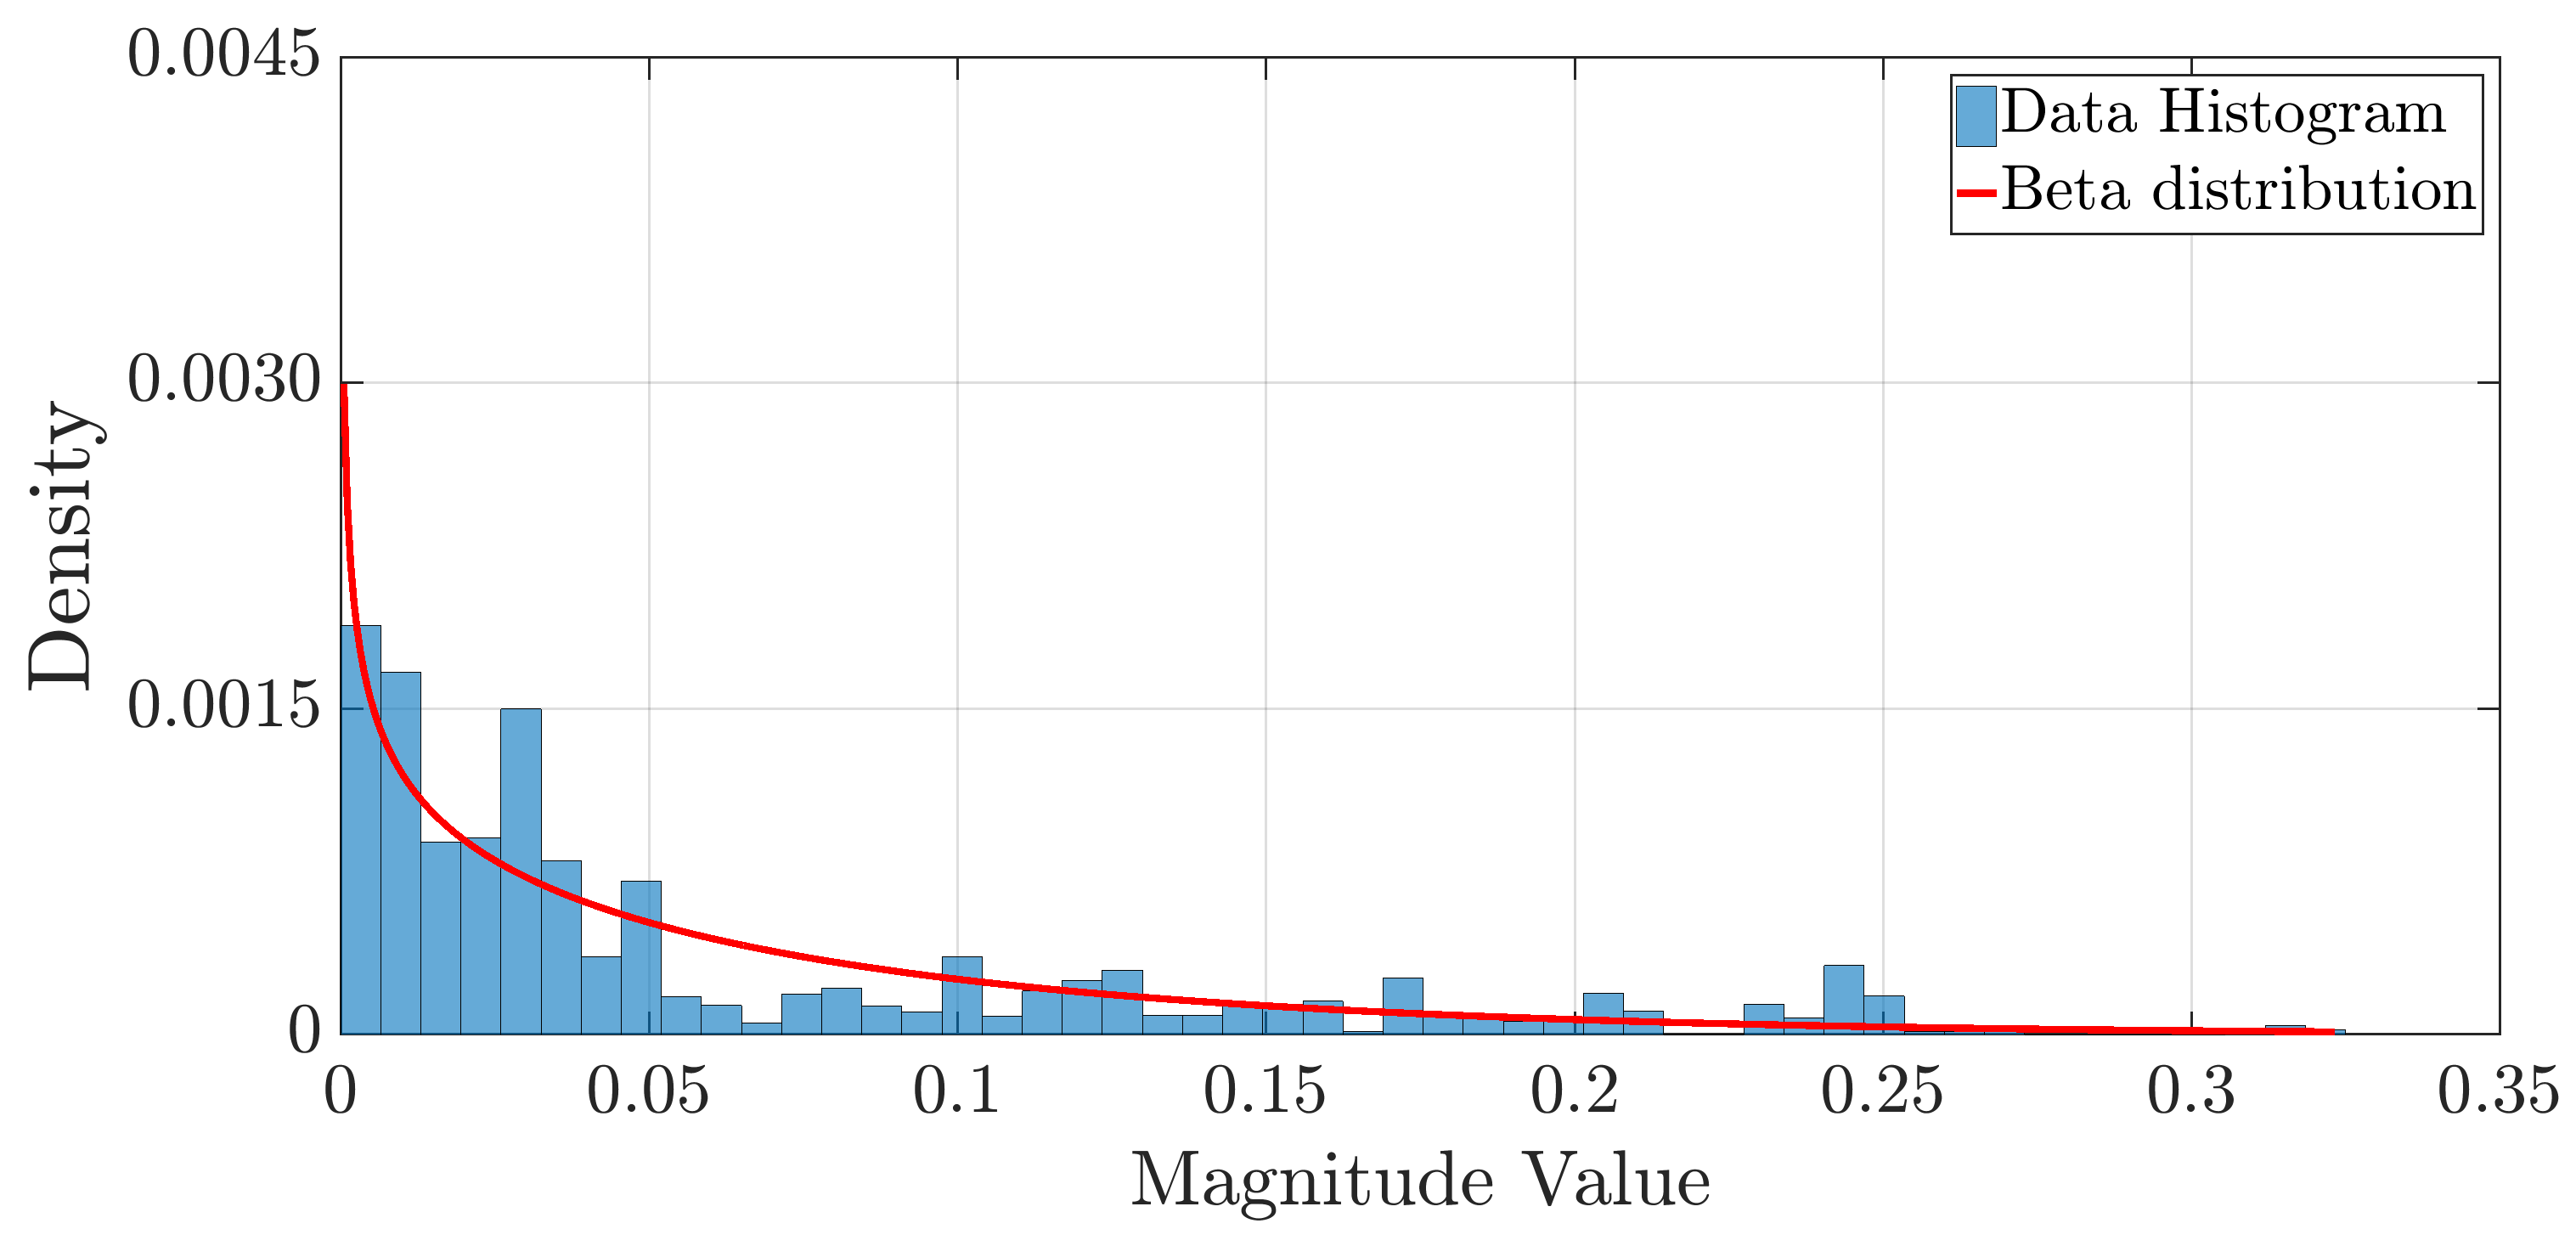
\includegraphics[width=0.49\textwidth]{images/Mag_hist_2.eps}
	\caption{The relative frequency of the magnitude of the valid \ac{CFR} estimates at the sample $k = 1067$ ($k\Delta f= 52.1$~MHz) and the modeling based on the Beta distribution.}
	\label{mag_example}
\end{figure}

\begin{figure}[h!]
	\centering
	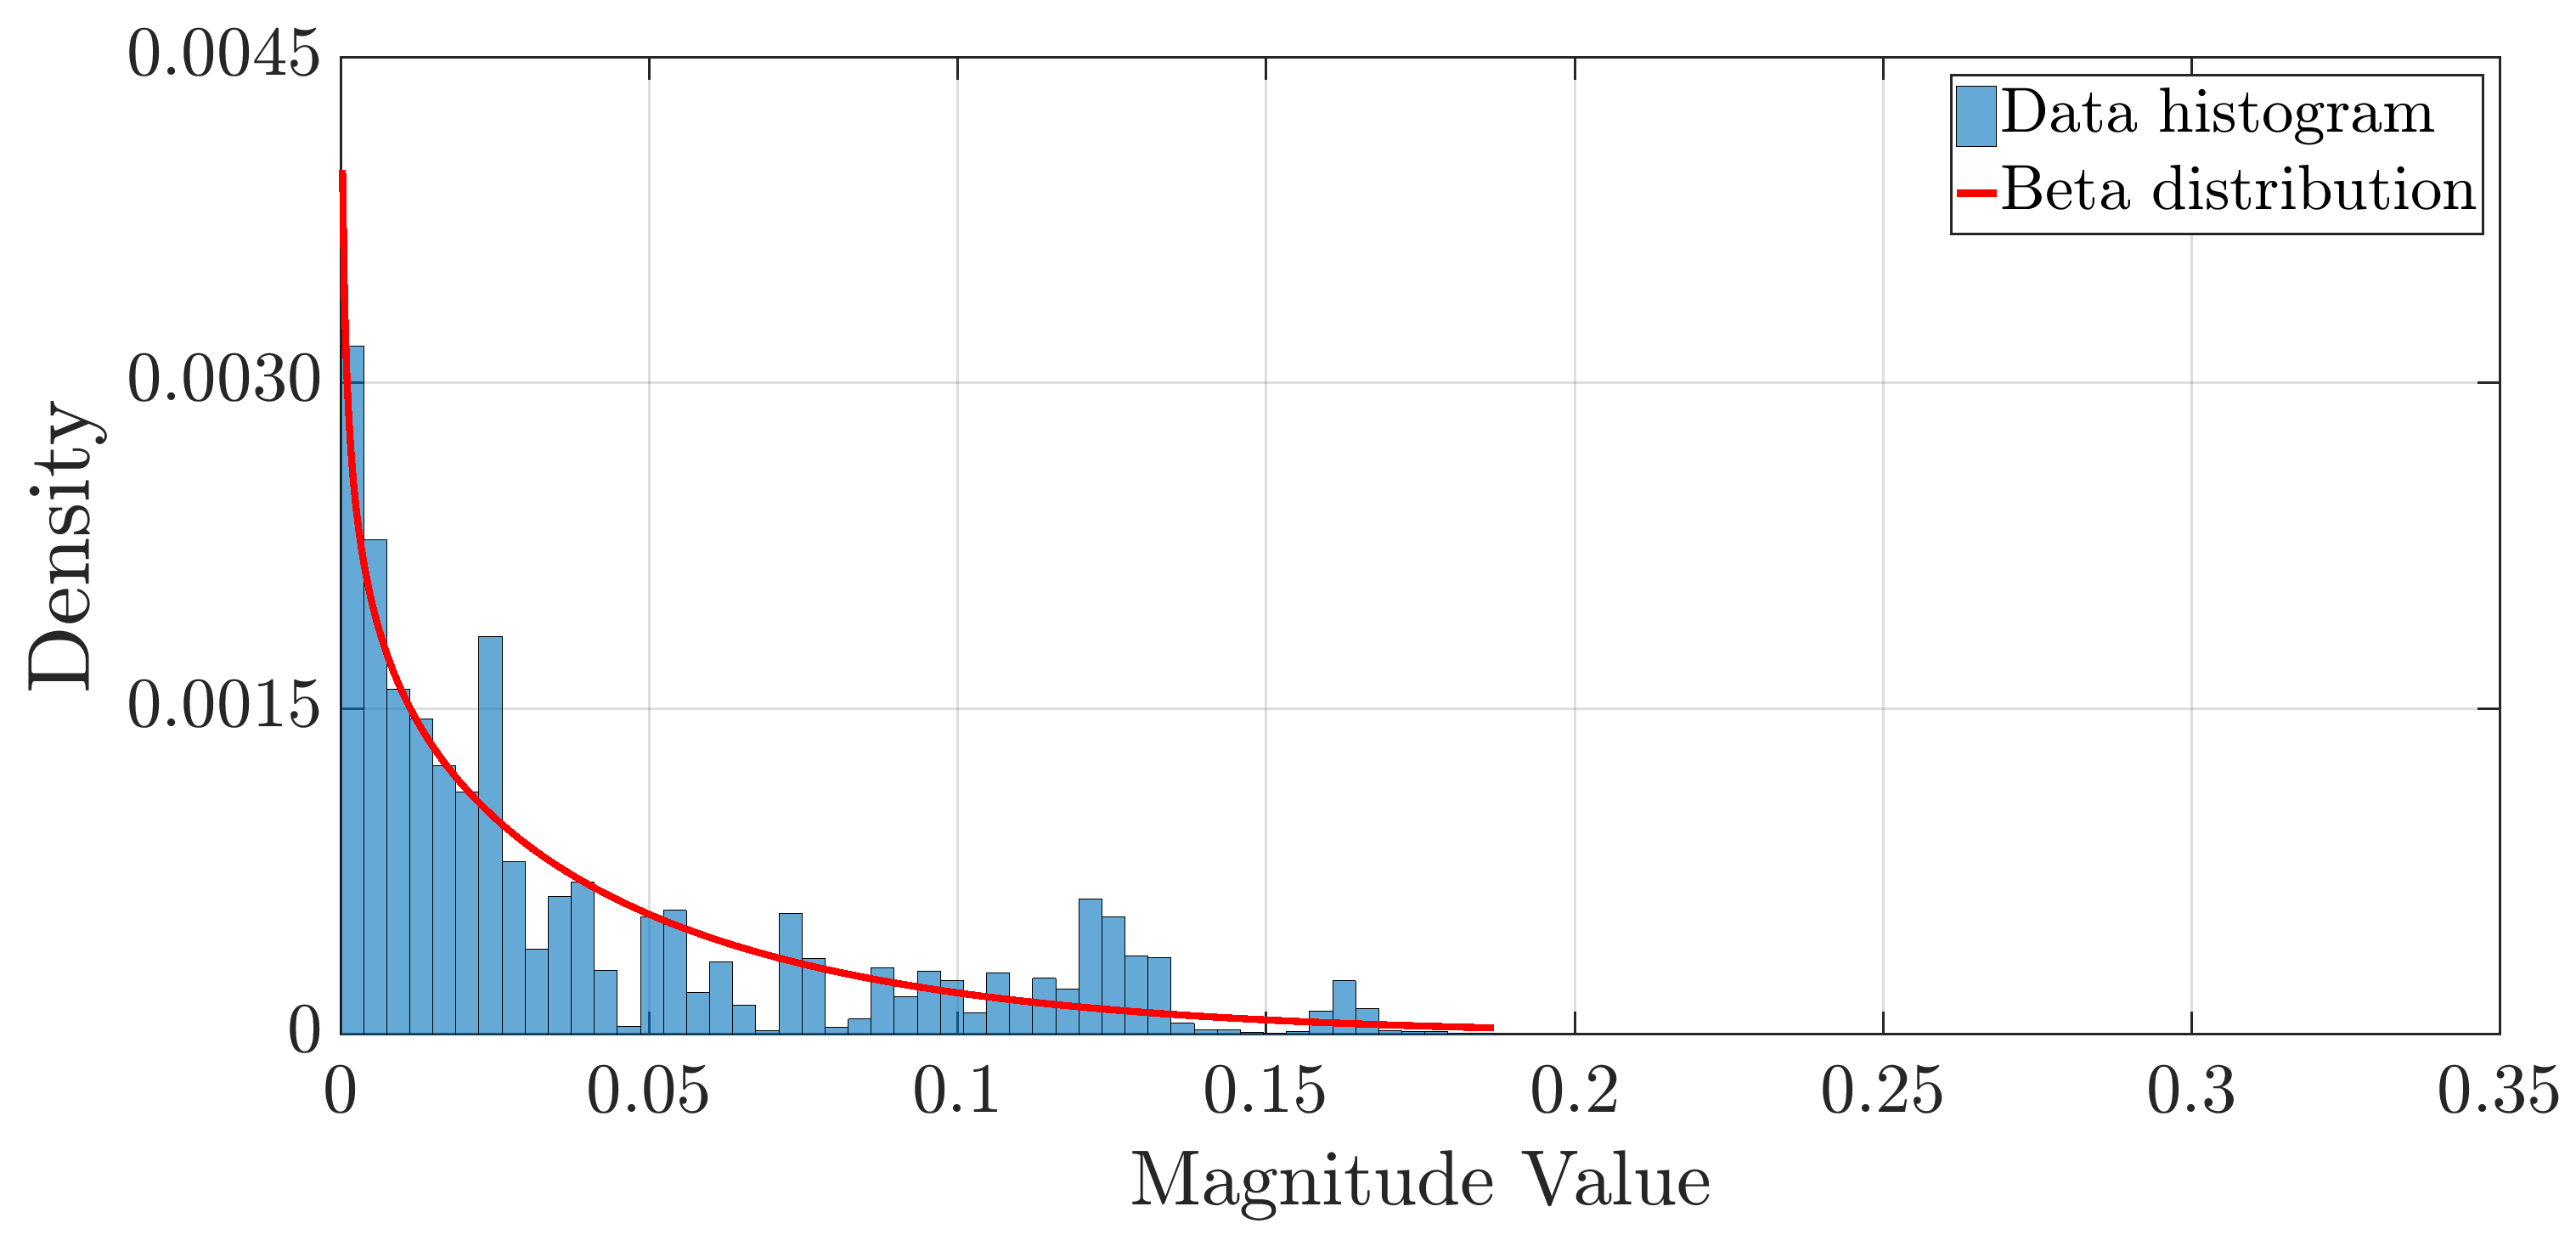
\includegraphics[width=0.49\textwidth]{images/Mag_hist2_2.eps}
	\caption{The relative frequency of the magnitude of the valid \ac{CFR} estimates at the sample $k = 1600$ ($k\Delta f= 78.1$~MHz) and the modeling based on the Beta distribution.}
	\label{mag_example2}
\end{figure}

By interpolating the parameters values $\alpha(k\Delta f)$ and $\beta(k\Delta f)$ of the Beta distributions, associated with each sampled valid \ac{CFR} estimates, using \textbf{Step \#4} of the proposed enhanced statistical modeling method, we obtain the continuous curves of parameters $\alpha(f)$ and $\beta(f)$, over the desired frequency band $(1.7-100$~MHz). Figs. \ref{Fit_alfa} and \ref{Fit_beta} show these curves for the parameters $\alpha(f)$ and $\beta(f)$ after the cubic Spline interpolation process is applied on the $L=19$ subintervals. For the sake of comparison, Fig. \ref{Fit_alfa_poli} shows the curves for parameter $\alpha(f)$ obtained, by applying the frequency domain interpolation technique detailed in \cite{mitra} and by using the interpolation technique discussed in \cite{Luis:AI} applied over $L=19$ subbands over the whole frequency bandwidth. On this figure is possible to notice the presence of edge effects that occurs in the boundaries between two polynomials, which are interpolating the values of the parameters in two consecutive frequency subbands. Furthermore, Table \ref{table_alfa} lists the cubic Spline coefficients for modeling the parameter $\alpha(f)$, of the valid \ac{CFR} magnitude. Similarly, Table \ref{table_beta} lists the cubic Spline coefficients for modeling the parameter $\beta(f)$. As a result, the coefficients values, the waveforms  $\alpha(f)$ and $\beta(f)$, and the Beta distribution define the random process representing the magnitude of the valid \ac{CFR} estimates, named $|{\bf H}|$, in the continuous-frequency domain.

\begin{figure}[h]
	\centering
	\psfrag{Interval Boundsaa}[c][c][0.7]{Interval Bounds}
	\psfrag{AAA}[c][c][0.7]{~~~~~~$\alpha(k \Delta f)$}
	\psfrag{BBB}[c][c][0.7]{~~$\hat{\alpha}(f)$}
	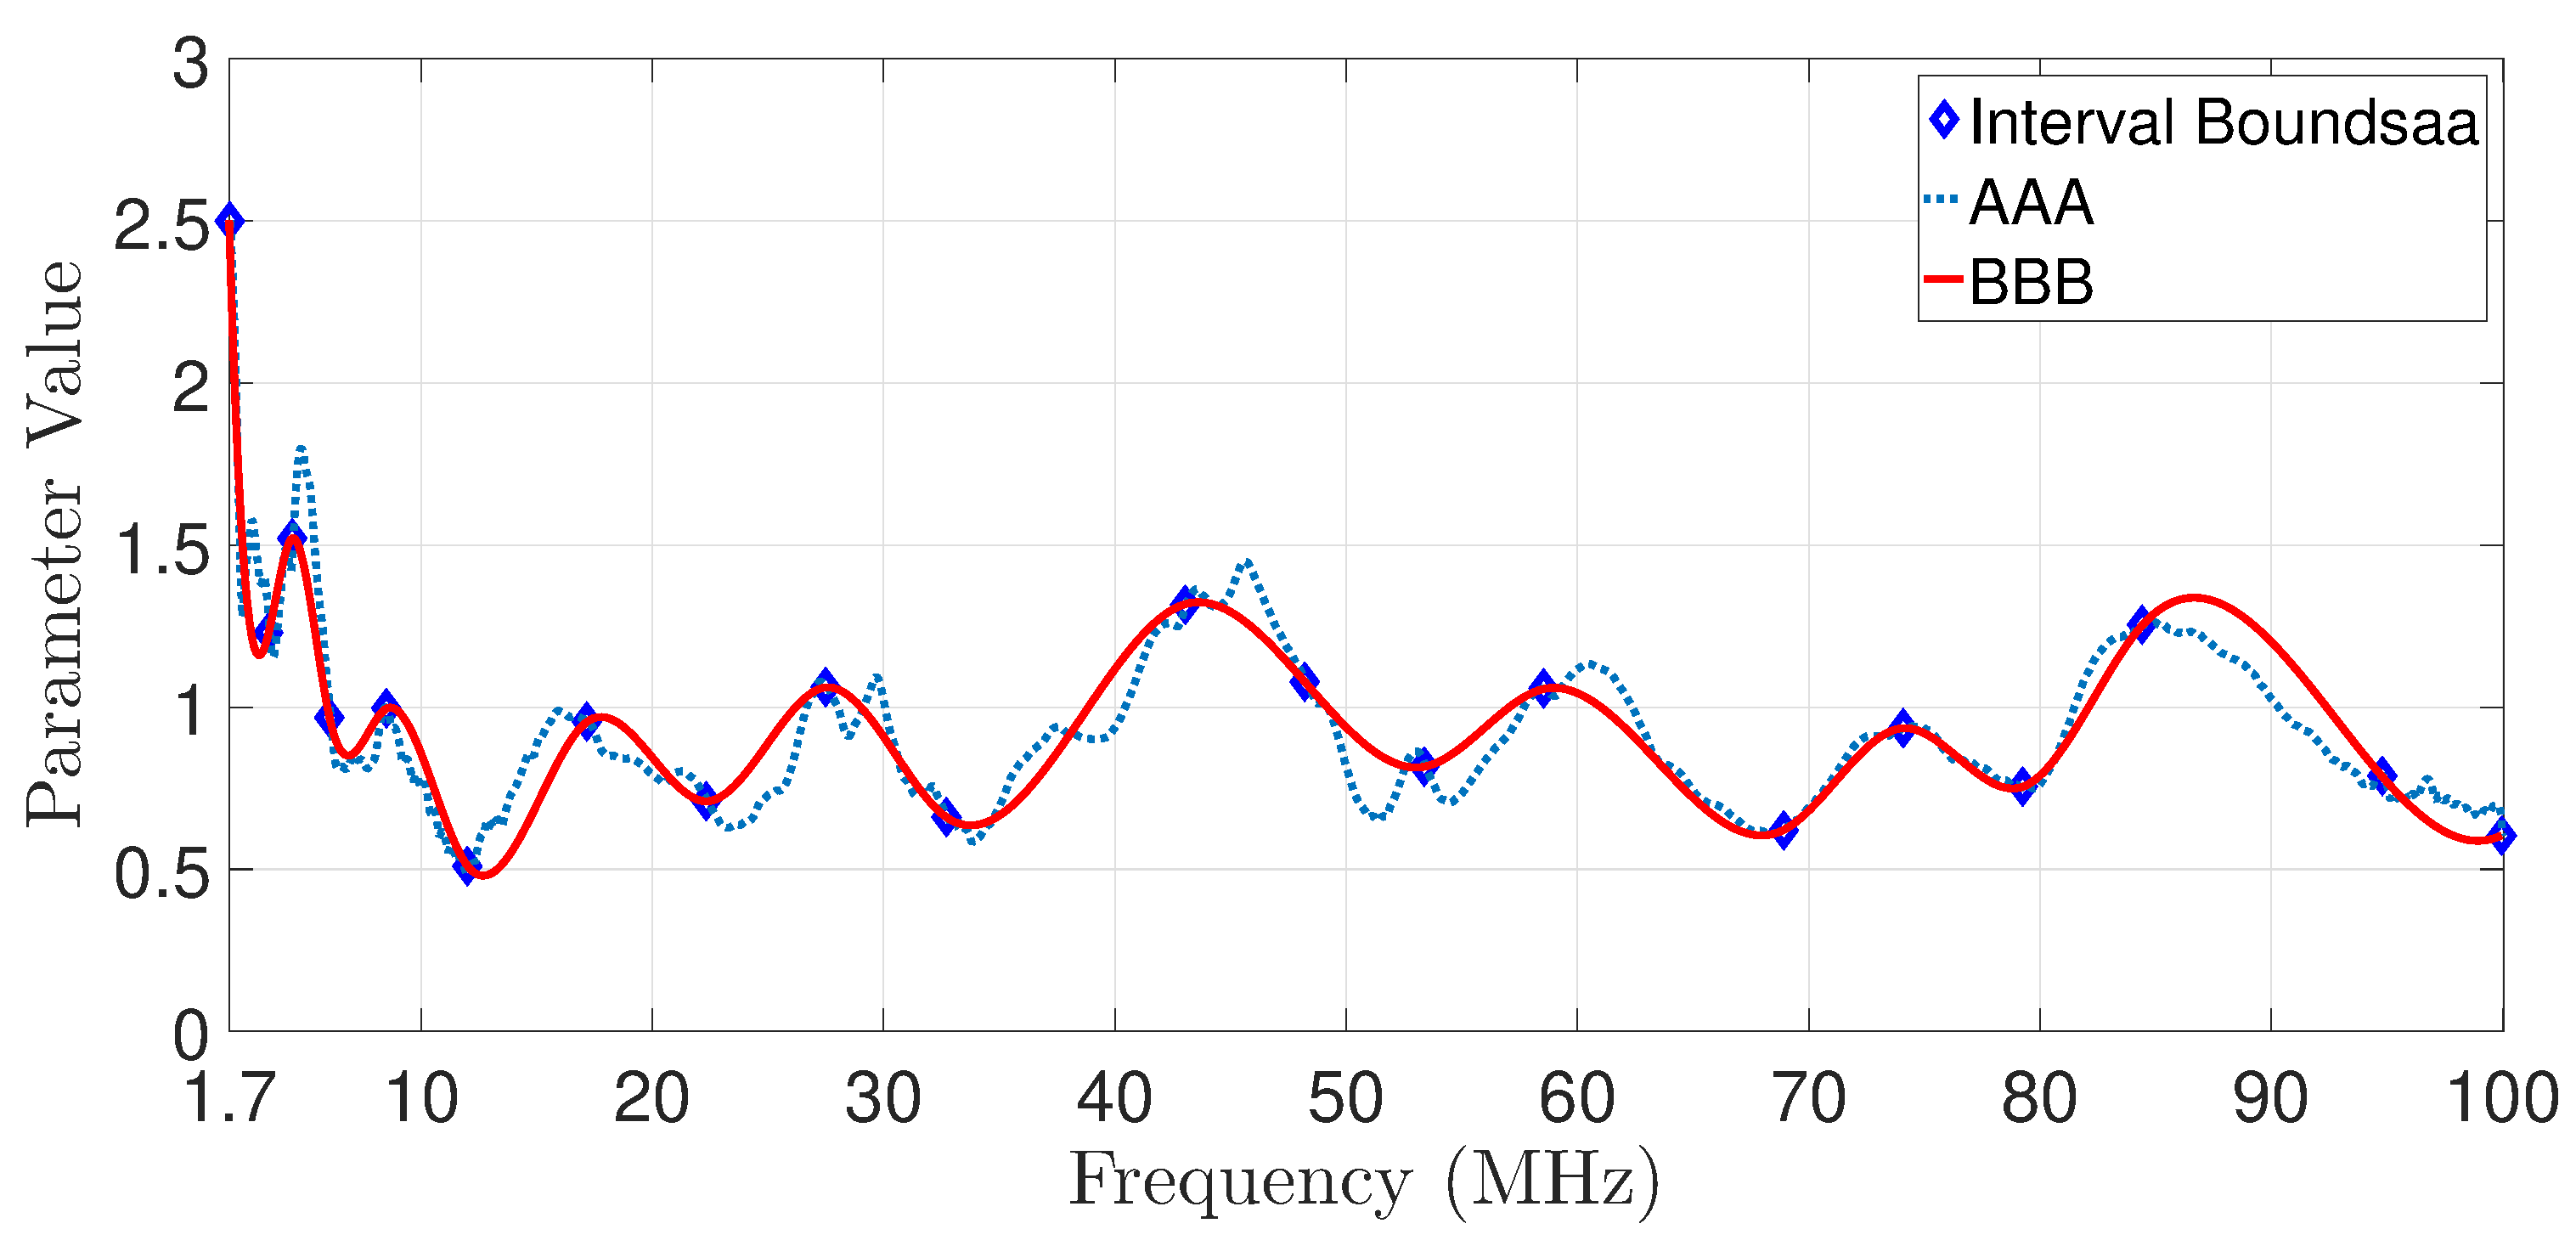
\includegraphics[width=0.49\textwidth]{images/Alfa_fit_1.7.eps}
	\caption{The result of the interpolation technique based on cubic Splines applied to obtain $\alpha(f) = \zeta_1(f)$ for the Beta distribution ($\alpha(k \Delta f)$ are the original values of the parameter and $\hat{\alpha}(f)$ is the interpolated curve).}
	\label{Fit_alfa}
\end{figure}

\begin{figure}[h]
	\centering
	\psfrag{Interval Subbandsaa}[c][c][0.7]{Interval Bounds$~~~$}
	\psfrag{AAA}[c][c][0.7]{$~~~~~{\alpha}(k \Delta f)$}
	\psfrag{BBB}[c][c][0.7]{$~~~~~~~~~~~~~~~l^{th}$ Polynomial}
	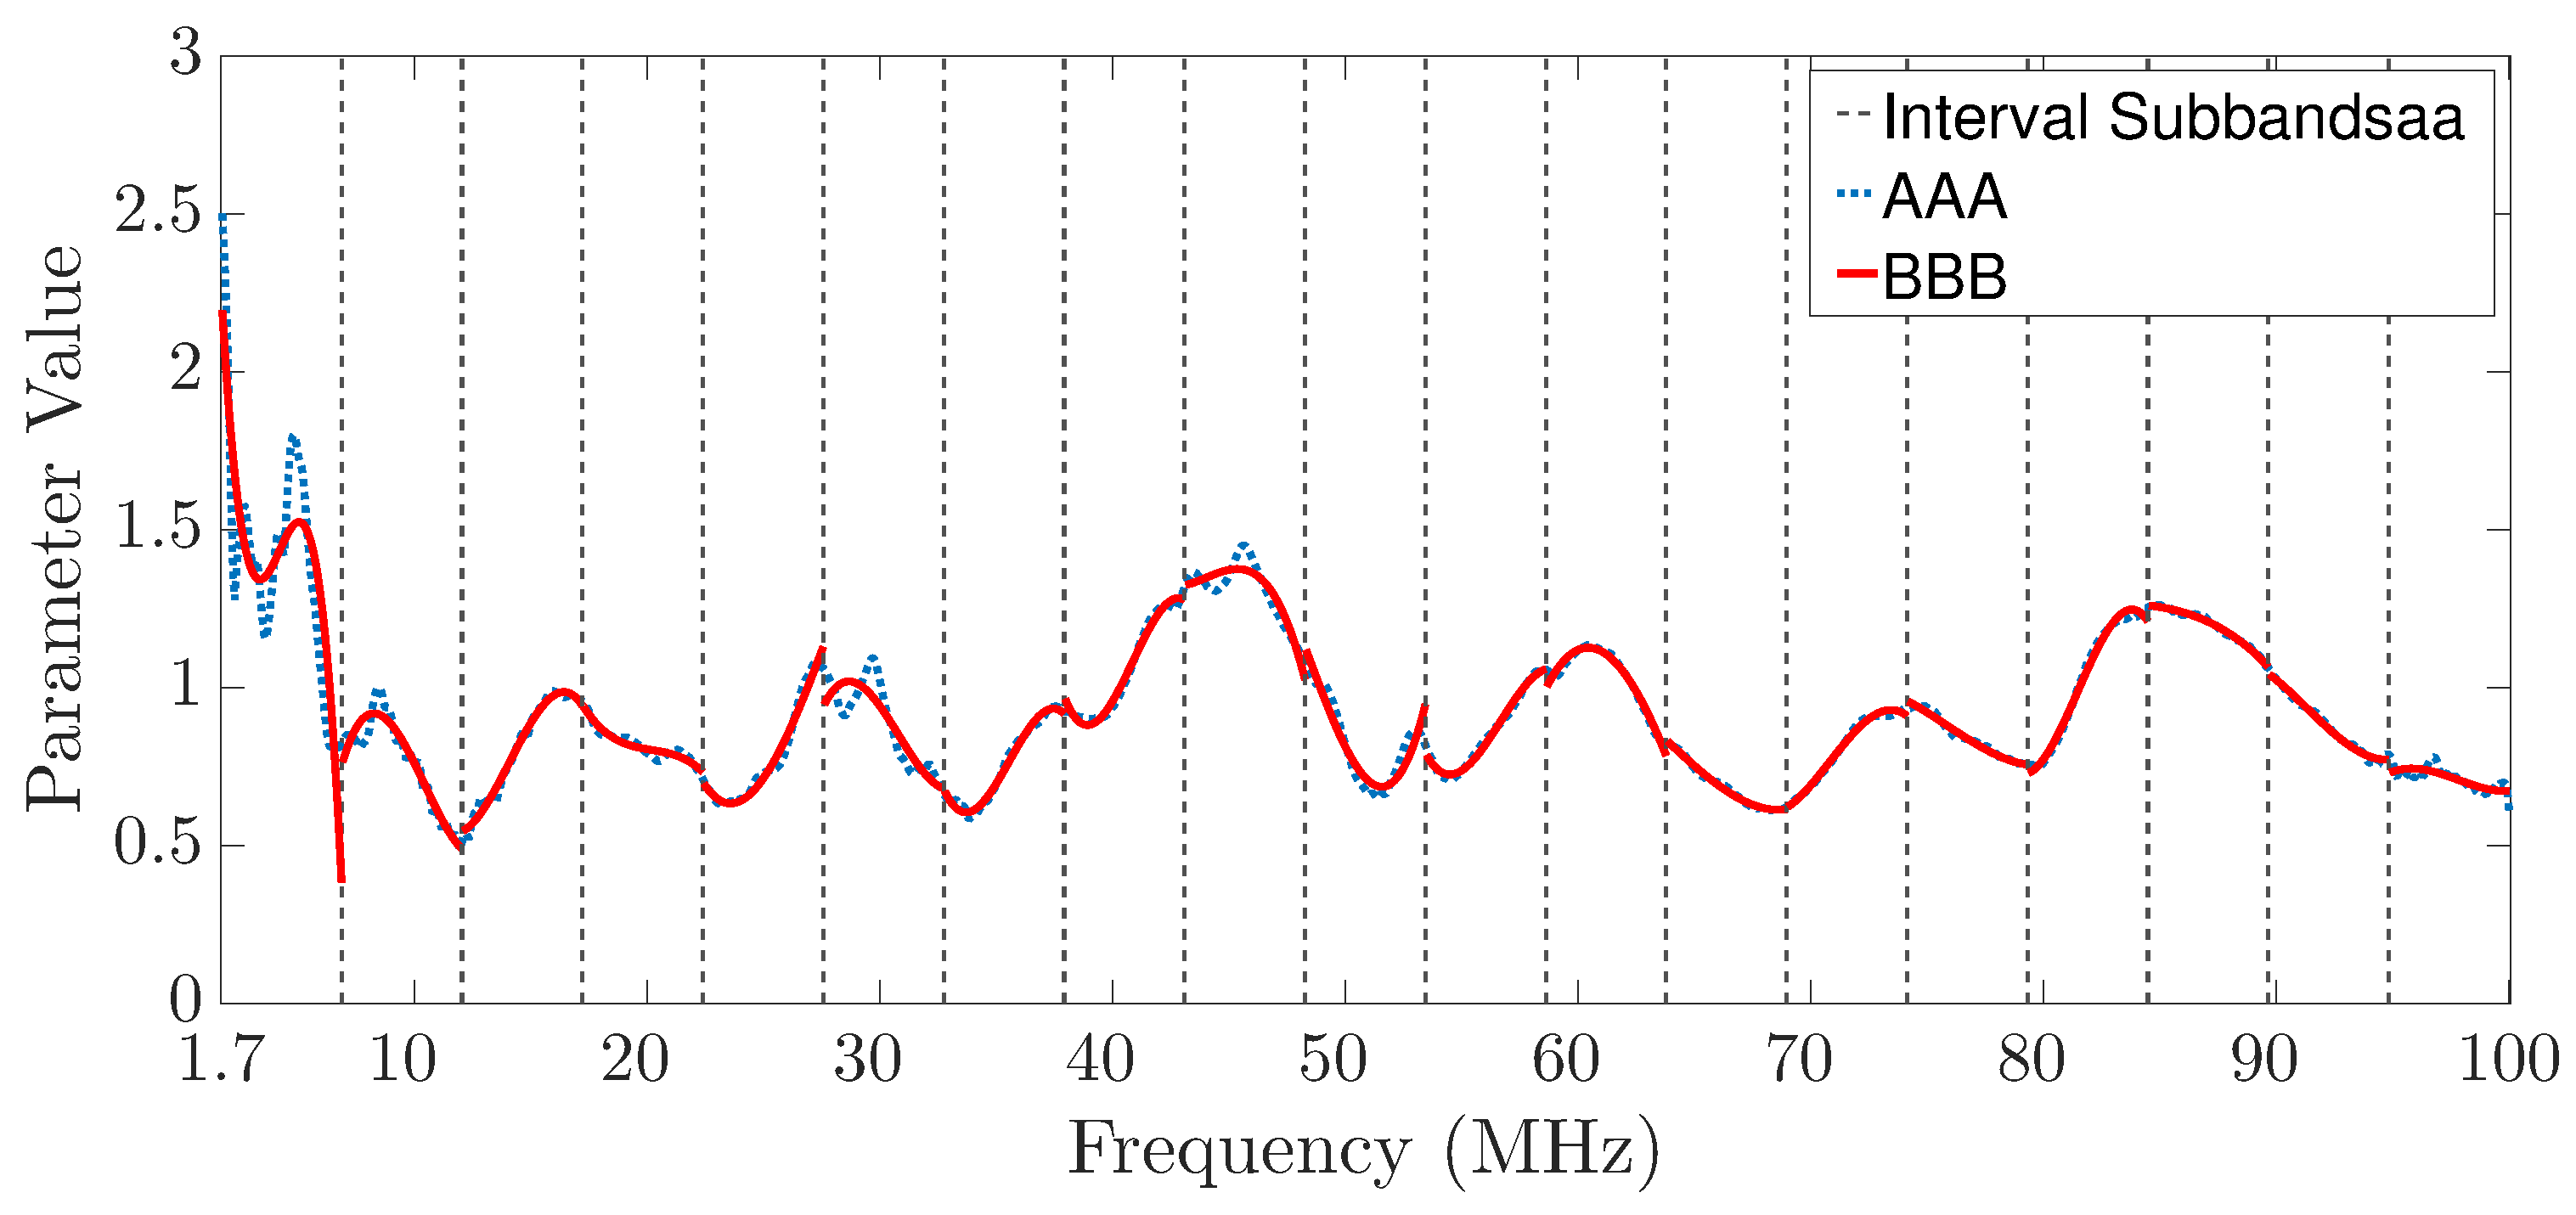
\includegraphics[width=0.49\textwidth]{images/SPLINE_Polynomials.eps}
	\caption{The result of the interpolation technique based on cubic Splines applied to obtain $\alpha(f)=\zeta_1(f)$ for the Beta distribution (${\alpha}(k \Delta f)$ are the original values of the parameter and $\hat{\alpha}(f)$ is the interpolated curve).}
	\label{Fit_alfa_poli}
\end{figure}

\begin{figure}[h!]
	\centering
	\psfrag{Interval Boundsaa}[c][c][0.7]{Interval Bounds}
	\psfrag{AAA}[c][c][0.7]{~~~~~~$\beta(k \Delta f)$}
	\psfrag{BBB}[c][c][0.7]{~~$\hat{\beta}(f)$}
	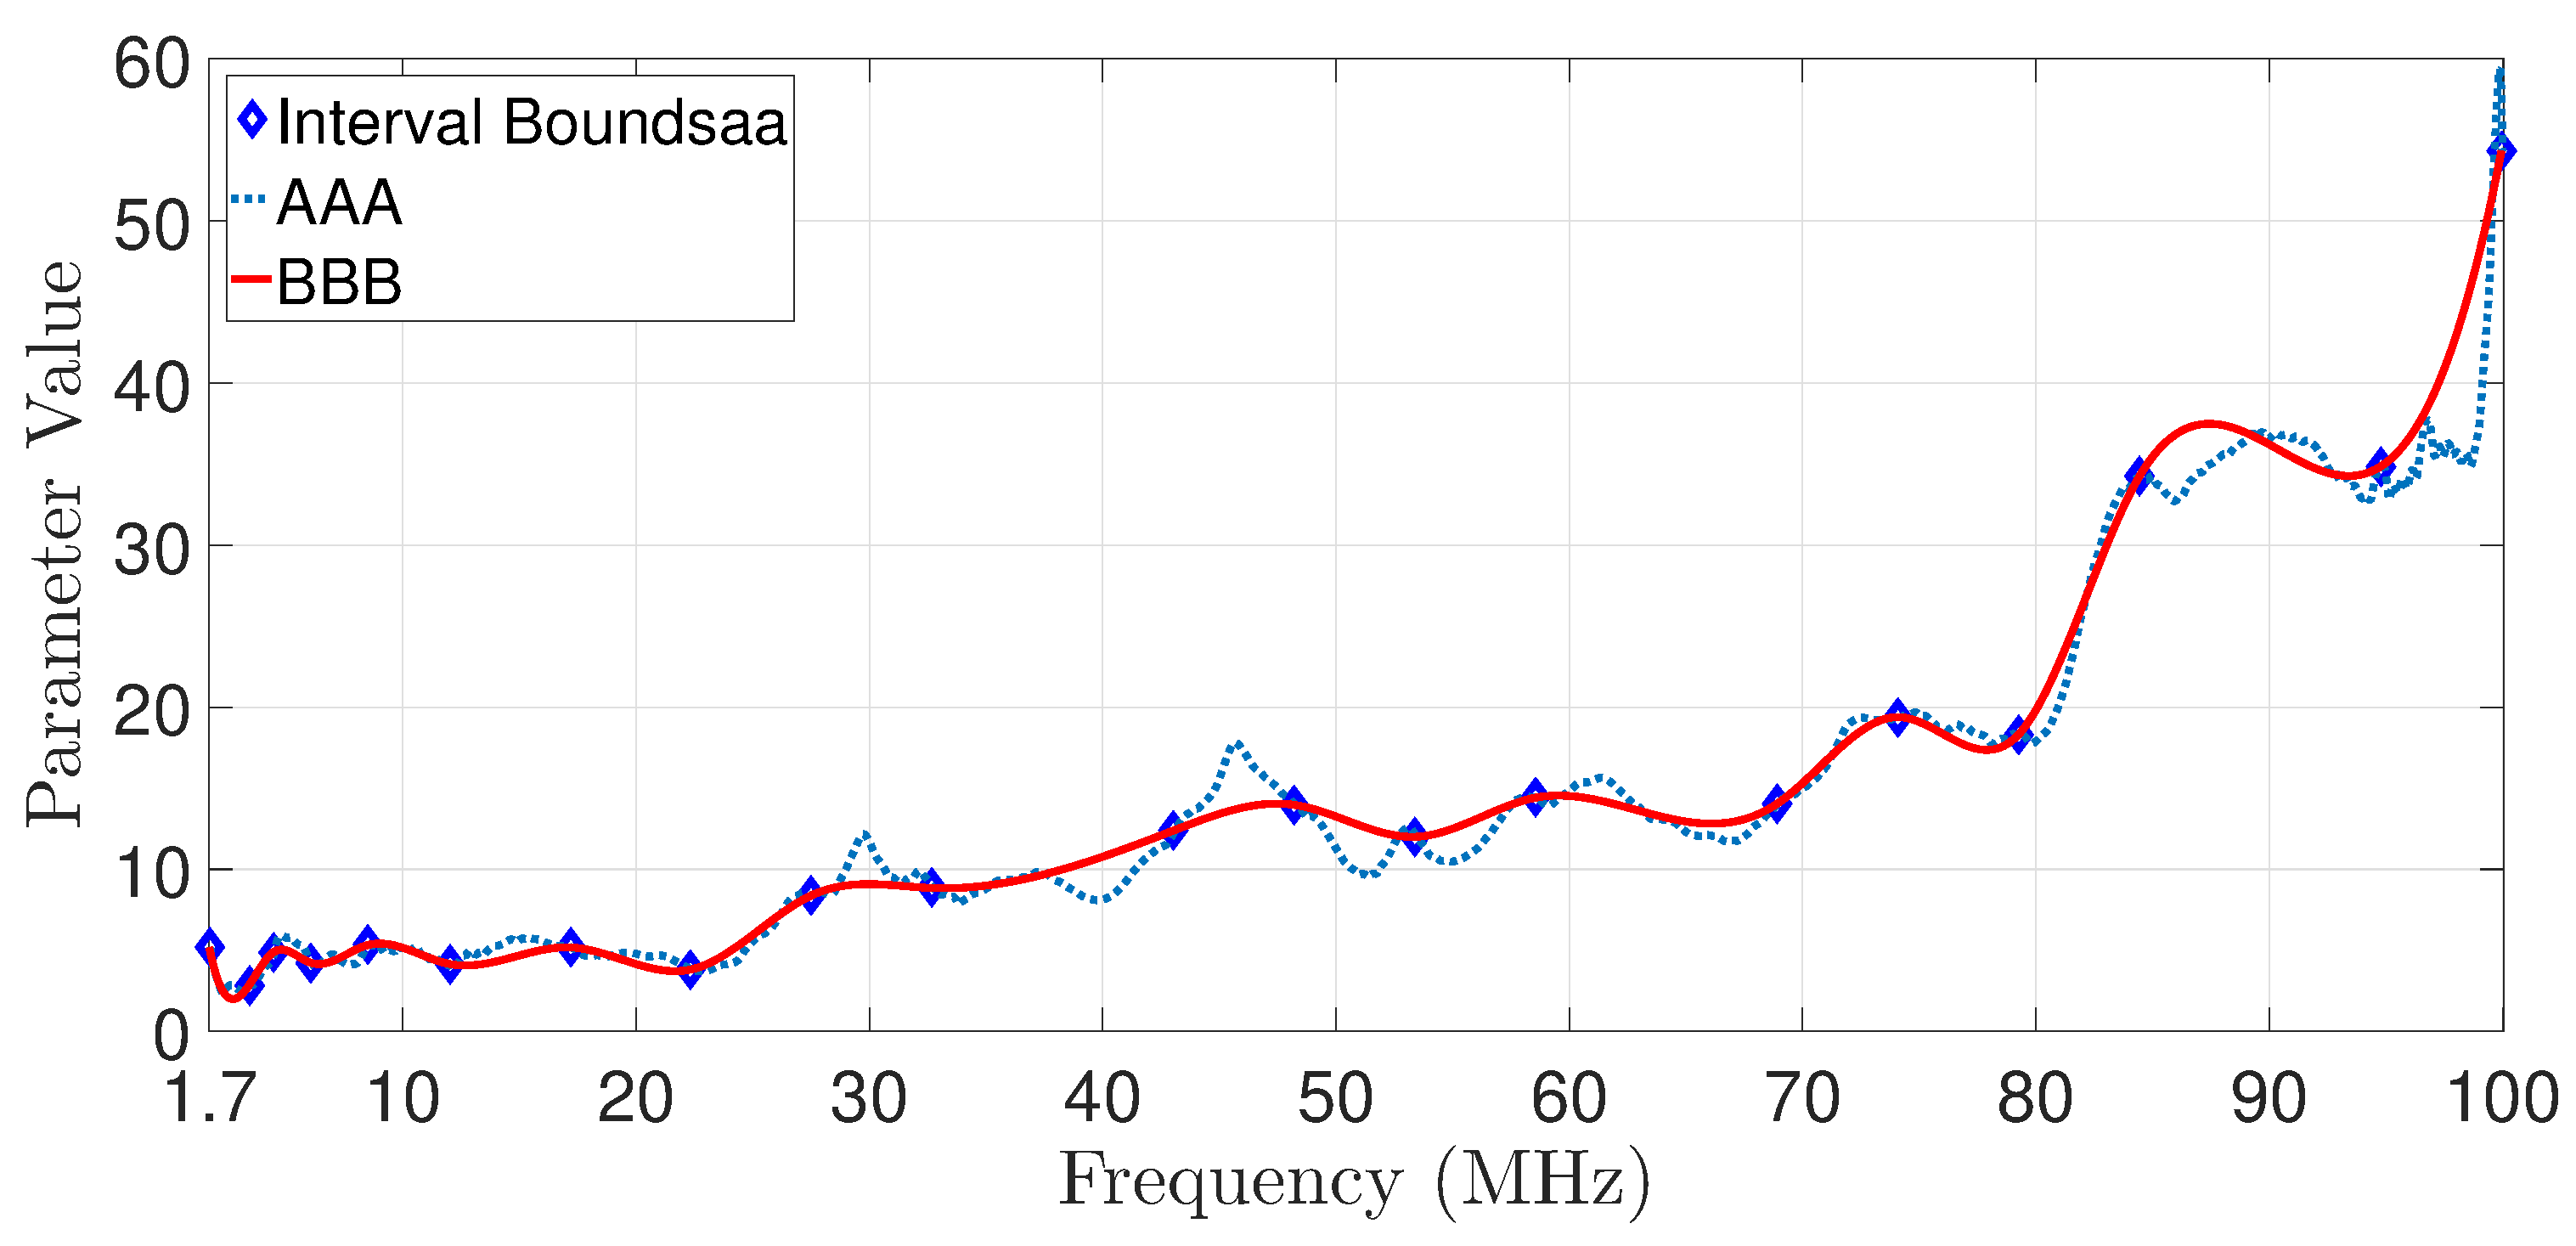
\includegraphics[width=0.49\textwidth]{images/Beta_fit_1.7.eps}
	\caption{The result of the interpolation technique based on cubic Splines applied to obtain $\beta(f) = \zeta_2(f)$ for the Beta distribution ($\beta(k \Delta f)$ are the original values of the parameter and $\hat{\beta}(f)$ is the interpolated curve).}
	\label{Fit_beta}
\end{figure}

\subsection{Hybrid PLC-WLC short path channels}\label{sec:MMHYBS}

 Fig. \ref{respfreqsW} shows five valid and consecutive estimates of the \ac{CFR} magnitude. Each valid \ac{CFR} estimate was obtained by averaging  $L_2=5$ consecutive \ac{CFR} estimates of the hybrid \ac{PLC}-\ac{WLC} \textit{short-path}. Note that the channel attenuation ranges from approximately $-40$~dB up to $-10$~dB and, in addition, a small time-varying behavior during a time interval shorter than $550\mu$s is observed, once each valid \ac{CFR} estimate covers a time interval equal to $\Delta T = L_2 T_{\textrm{sym}} \approx 115.2~\mu$s and, as a consequence, $5\Delta T = 576~\mu$s. 

\begin{figure}[h]
	\centering
	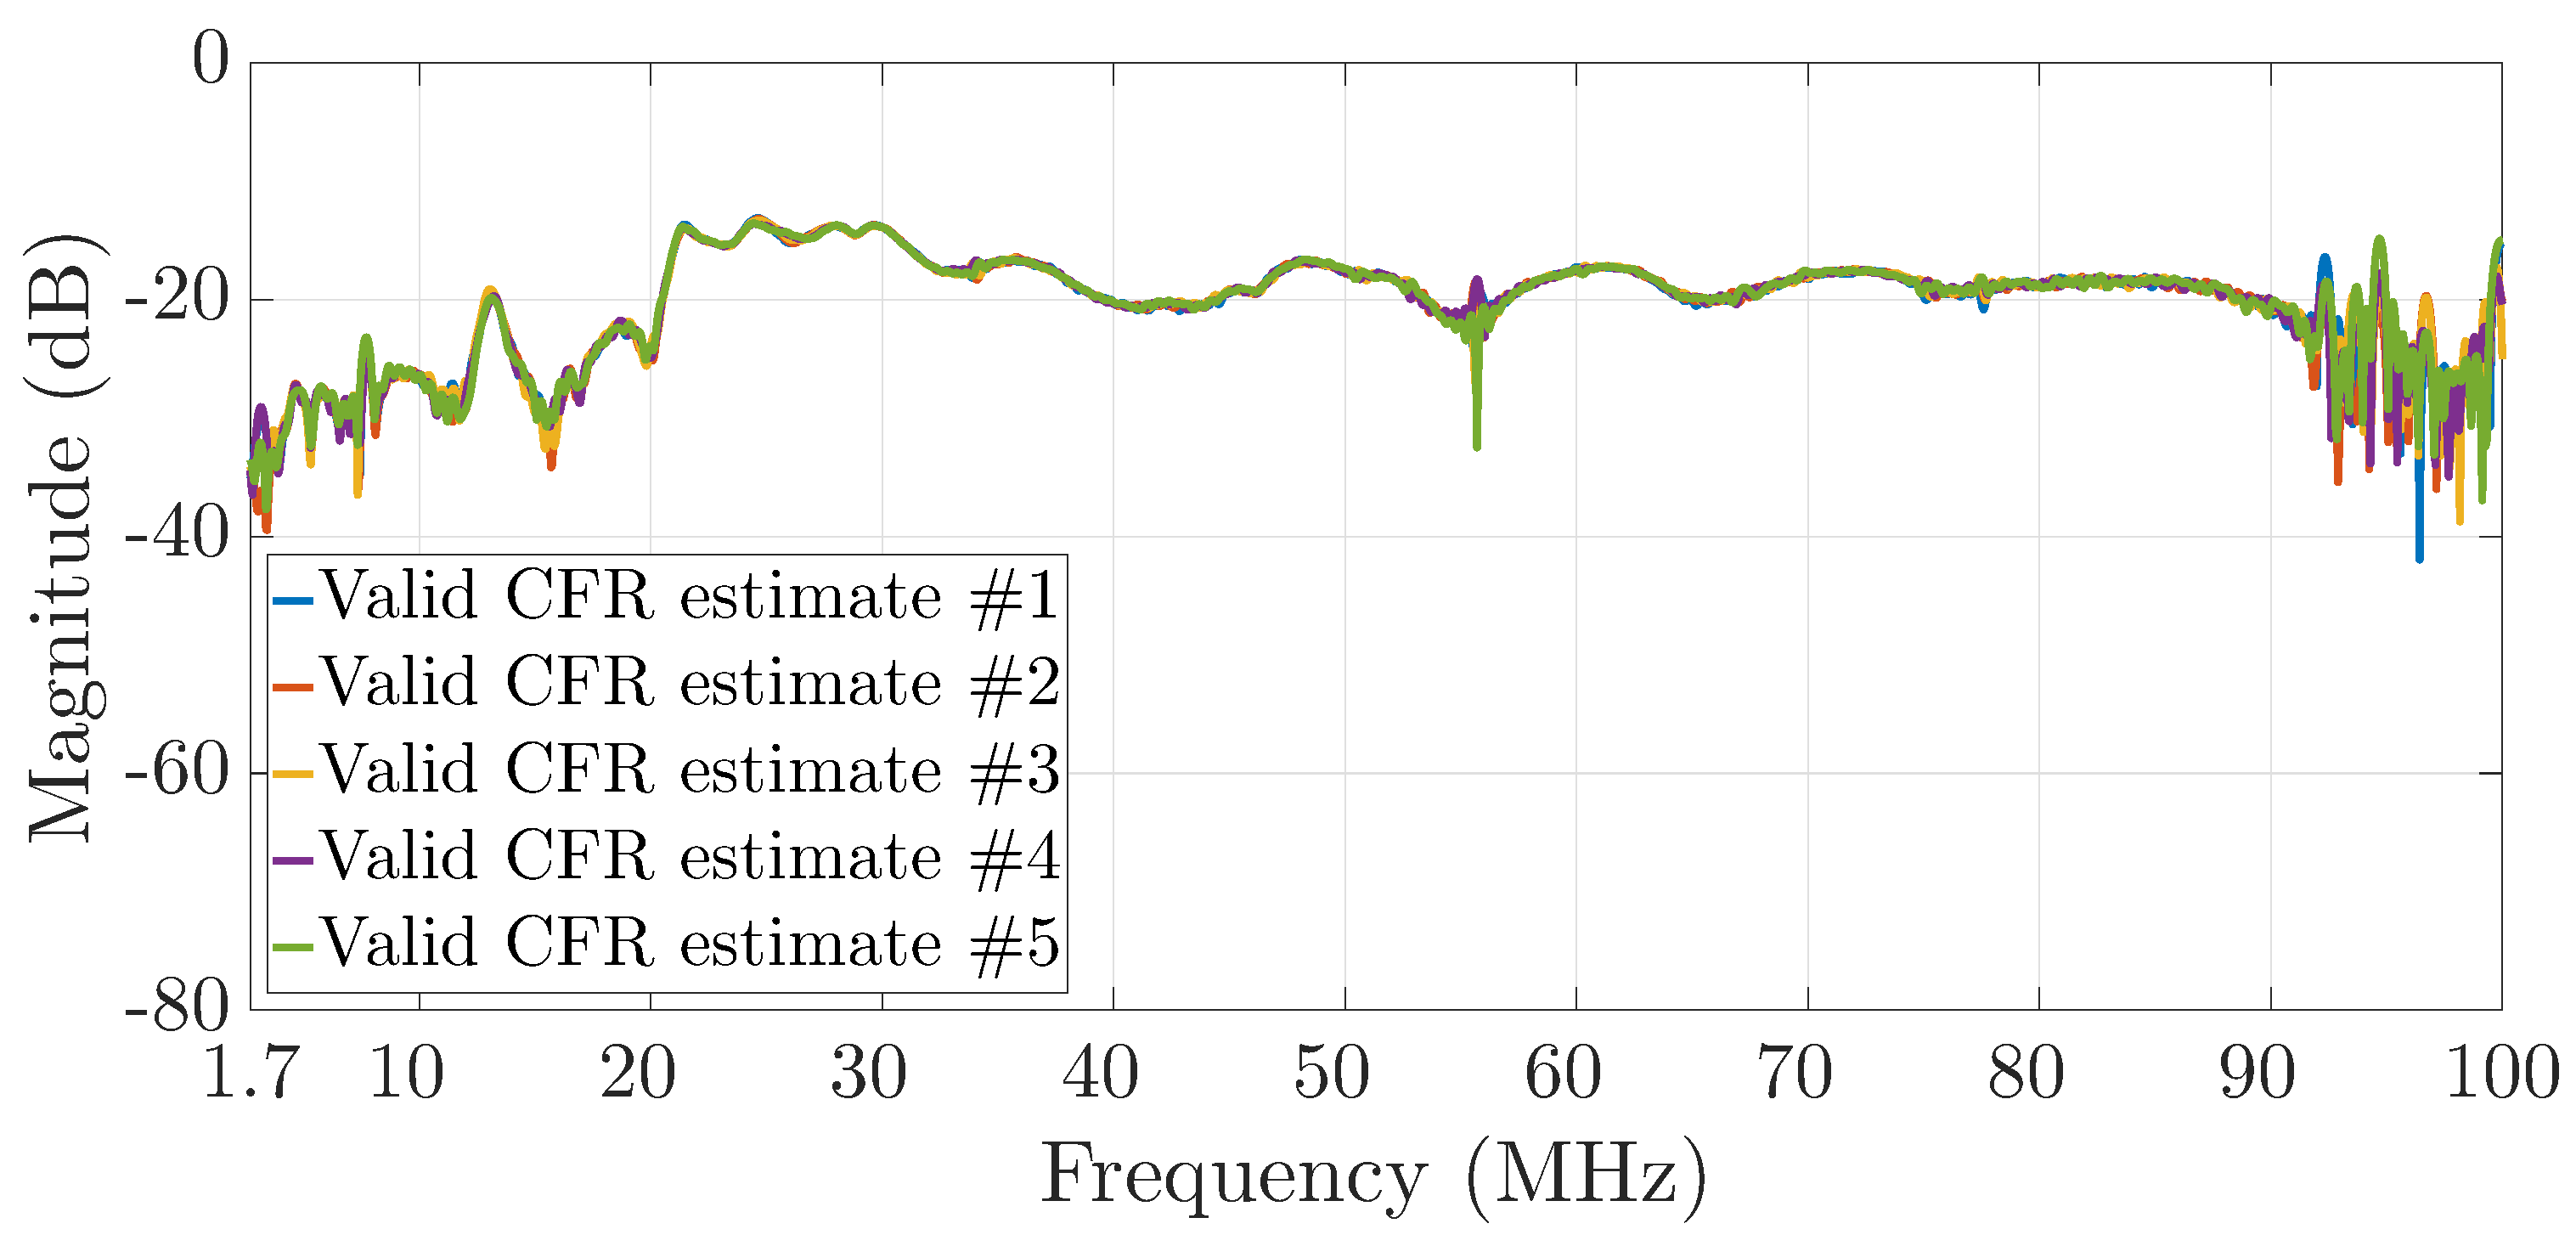
\includegraphics[width=0.49\textwidth]{images/respfreqsW.eps}
	\caption{Five consecutive and valid CFR Magnitudes of the measured in-home PLC channel.}
	\label{respfreqsW}
\end{figure}

Fig. \ref{MAG_percentsW} shows the relative frequency of statistical distributions that had modeled the magnitude of the hybrid \ac{PLC}-\ac{WLC} \textit{short-path} \ac{CFR} estimates. On these plots, it is noticeable a statistical distribution that models the majority of the magnitudes, once that in 54\% of the \ac{CFR} estimates the Log-normal distribution resulted in the best model. However, another different statistical distribution stands out as possible candidate to model the \ac{CFR} magnitudes, since in 30\% of the \ac{CFR} estimates, the Gamma distribution offered the best modeling. 

\begin{figure}[h!]
	\centering
	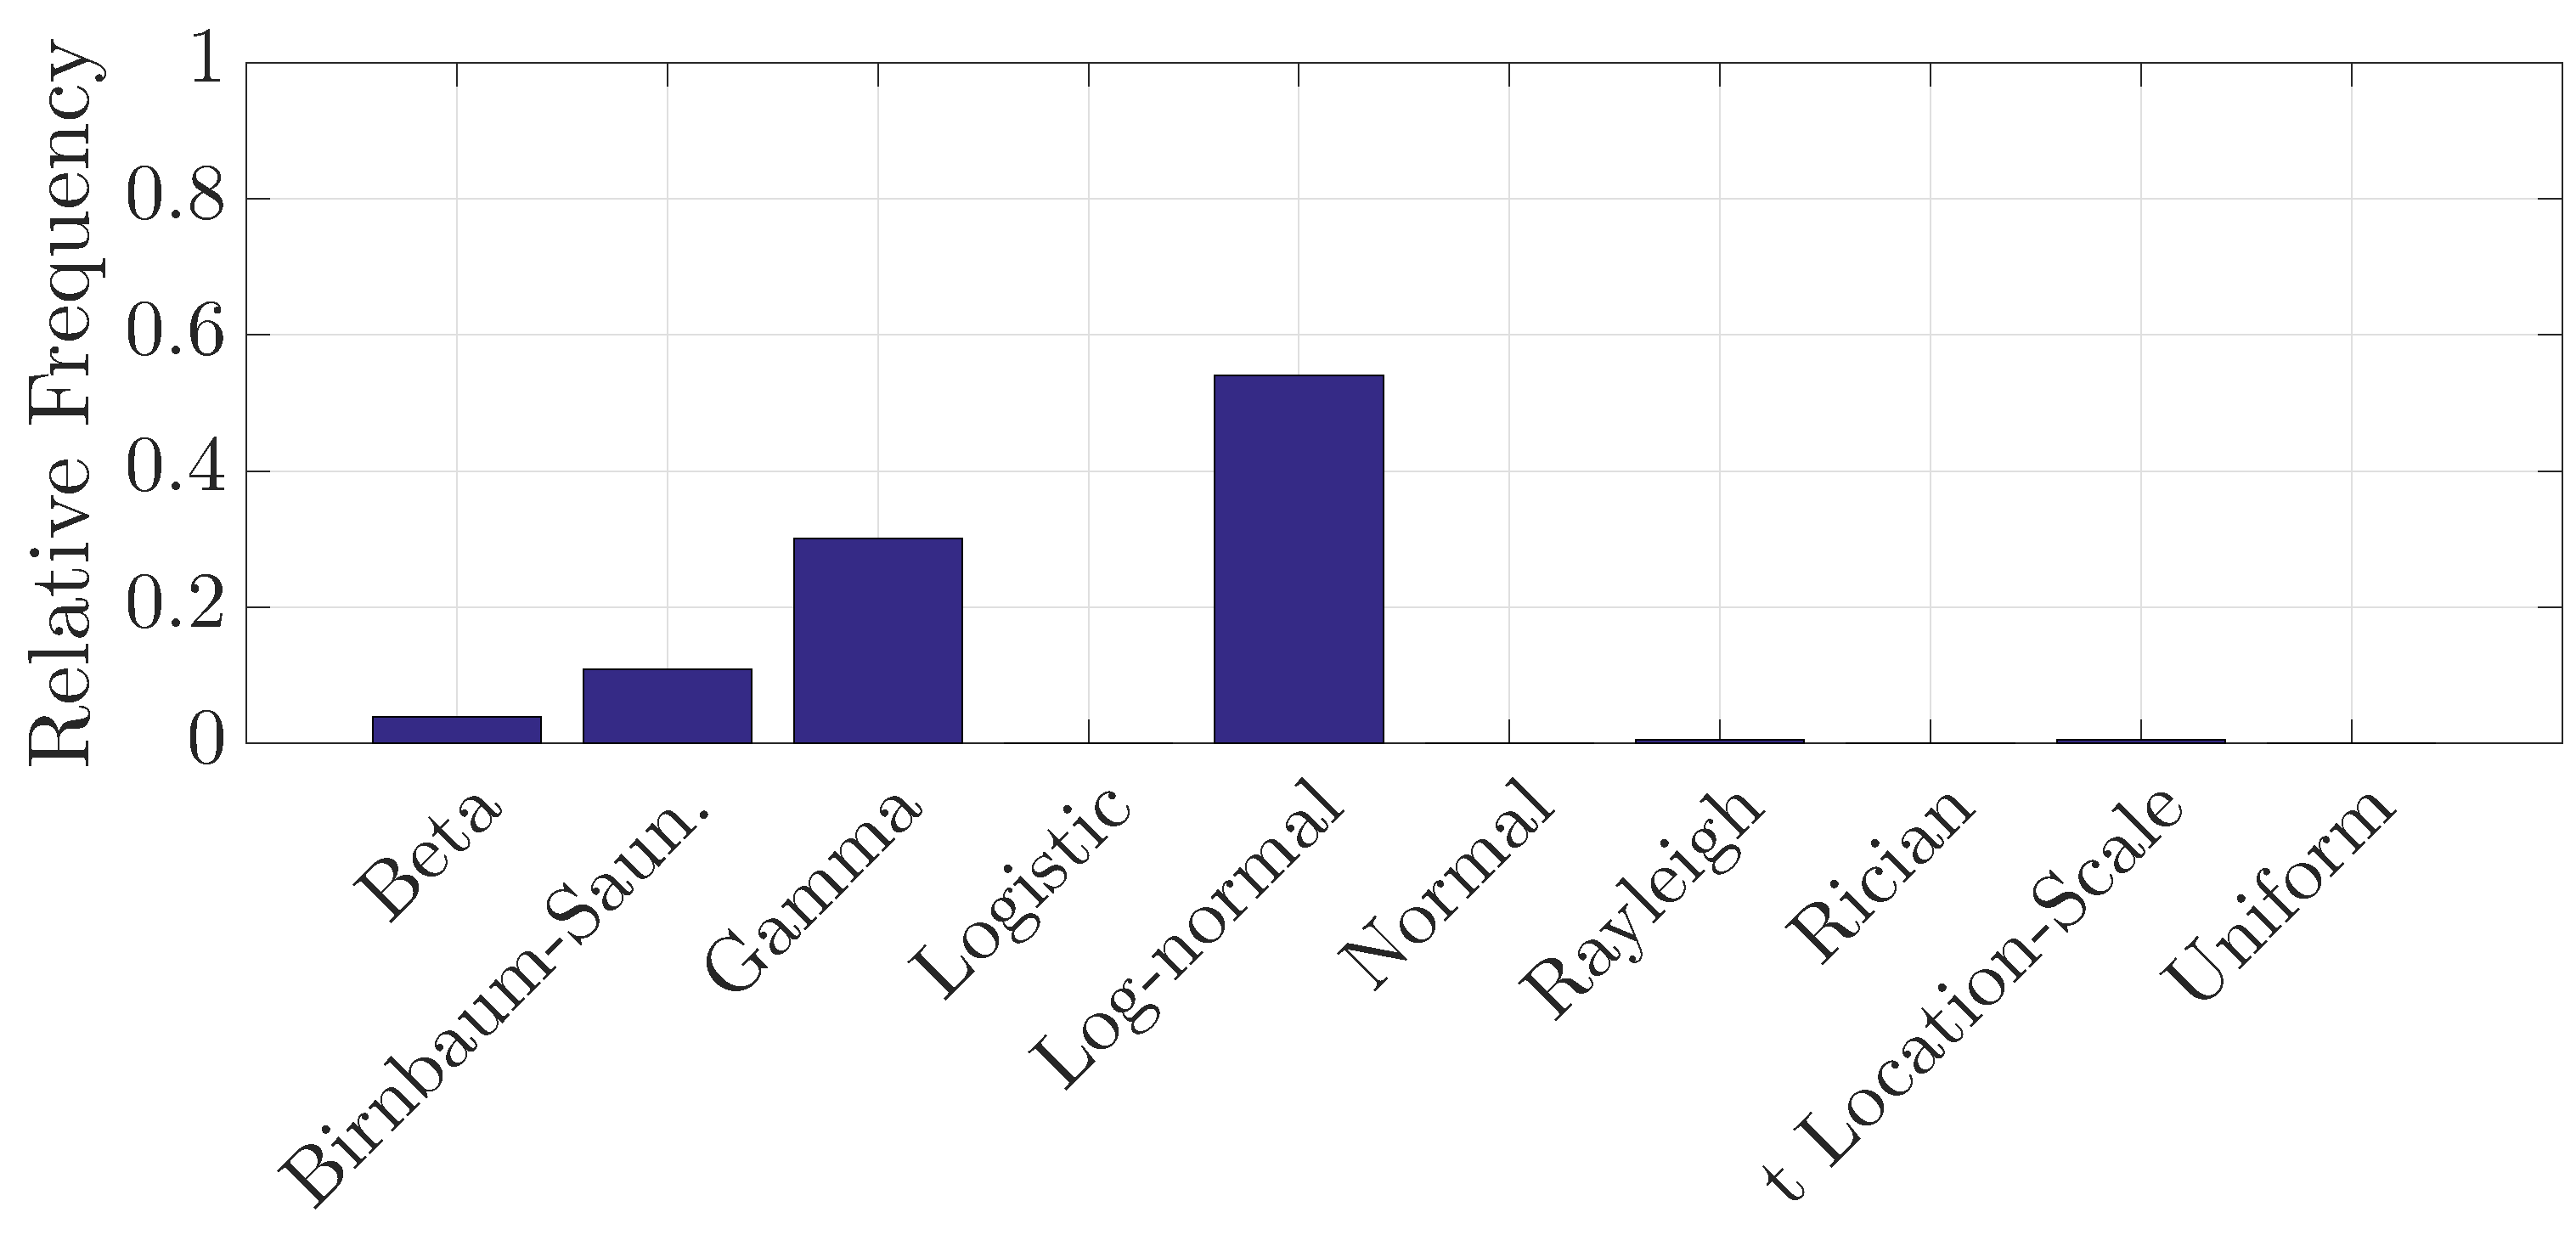
\includegraphics[width=0.49\textwidth]{images/MAG_percentsW.eps}
	\caption{The relative frequency associated with the chosen statistical distribution that best models the CFR magnitude in accord with the adopted criteria.}
	\label{MAG_percentsW}
\end{figure}

Similar to subsection \ref{sec:MMPLC}, (\ref{eq:log-lik}) was used in order to evaluate which of the two distributions is the best choice to model the magnitude component of the \ac{CFR} estimates. Fig. \ref{fig:Log_likesW} shows the values of  $\rho_{A}(f)$ for the two best statistical distributions candidates to model the magnitude of the valid \ac{CFR} estimates. These curves emphasize that both Log-normal and Gamma distributions achieved the minimum ratio over the \ac{MLE} criterion, in this scenario, the Log-normal distribution was chosen due to the large number of occurrence as the best model for the \ac{PLC}-\ac{WLC} \textit{short-path} \ac{CFR} magnitudes, as shown in Fig. \ref{MAG_percentsW}. In other words, the magnitude of the valid \ac{CFR} estimates of in-home hybrid \ac{PLC}-\ac{WLC} \textit{short-path} channels is modeled by using only one statistical distribution (i.e., the Log-normal distribution).

\begin{figure}[h!]
	\centering
	\psfrag{AAA}[c][c][1.0]{$\rho_{A} (f)$}
	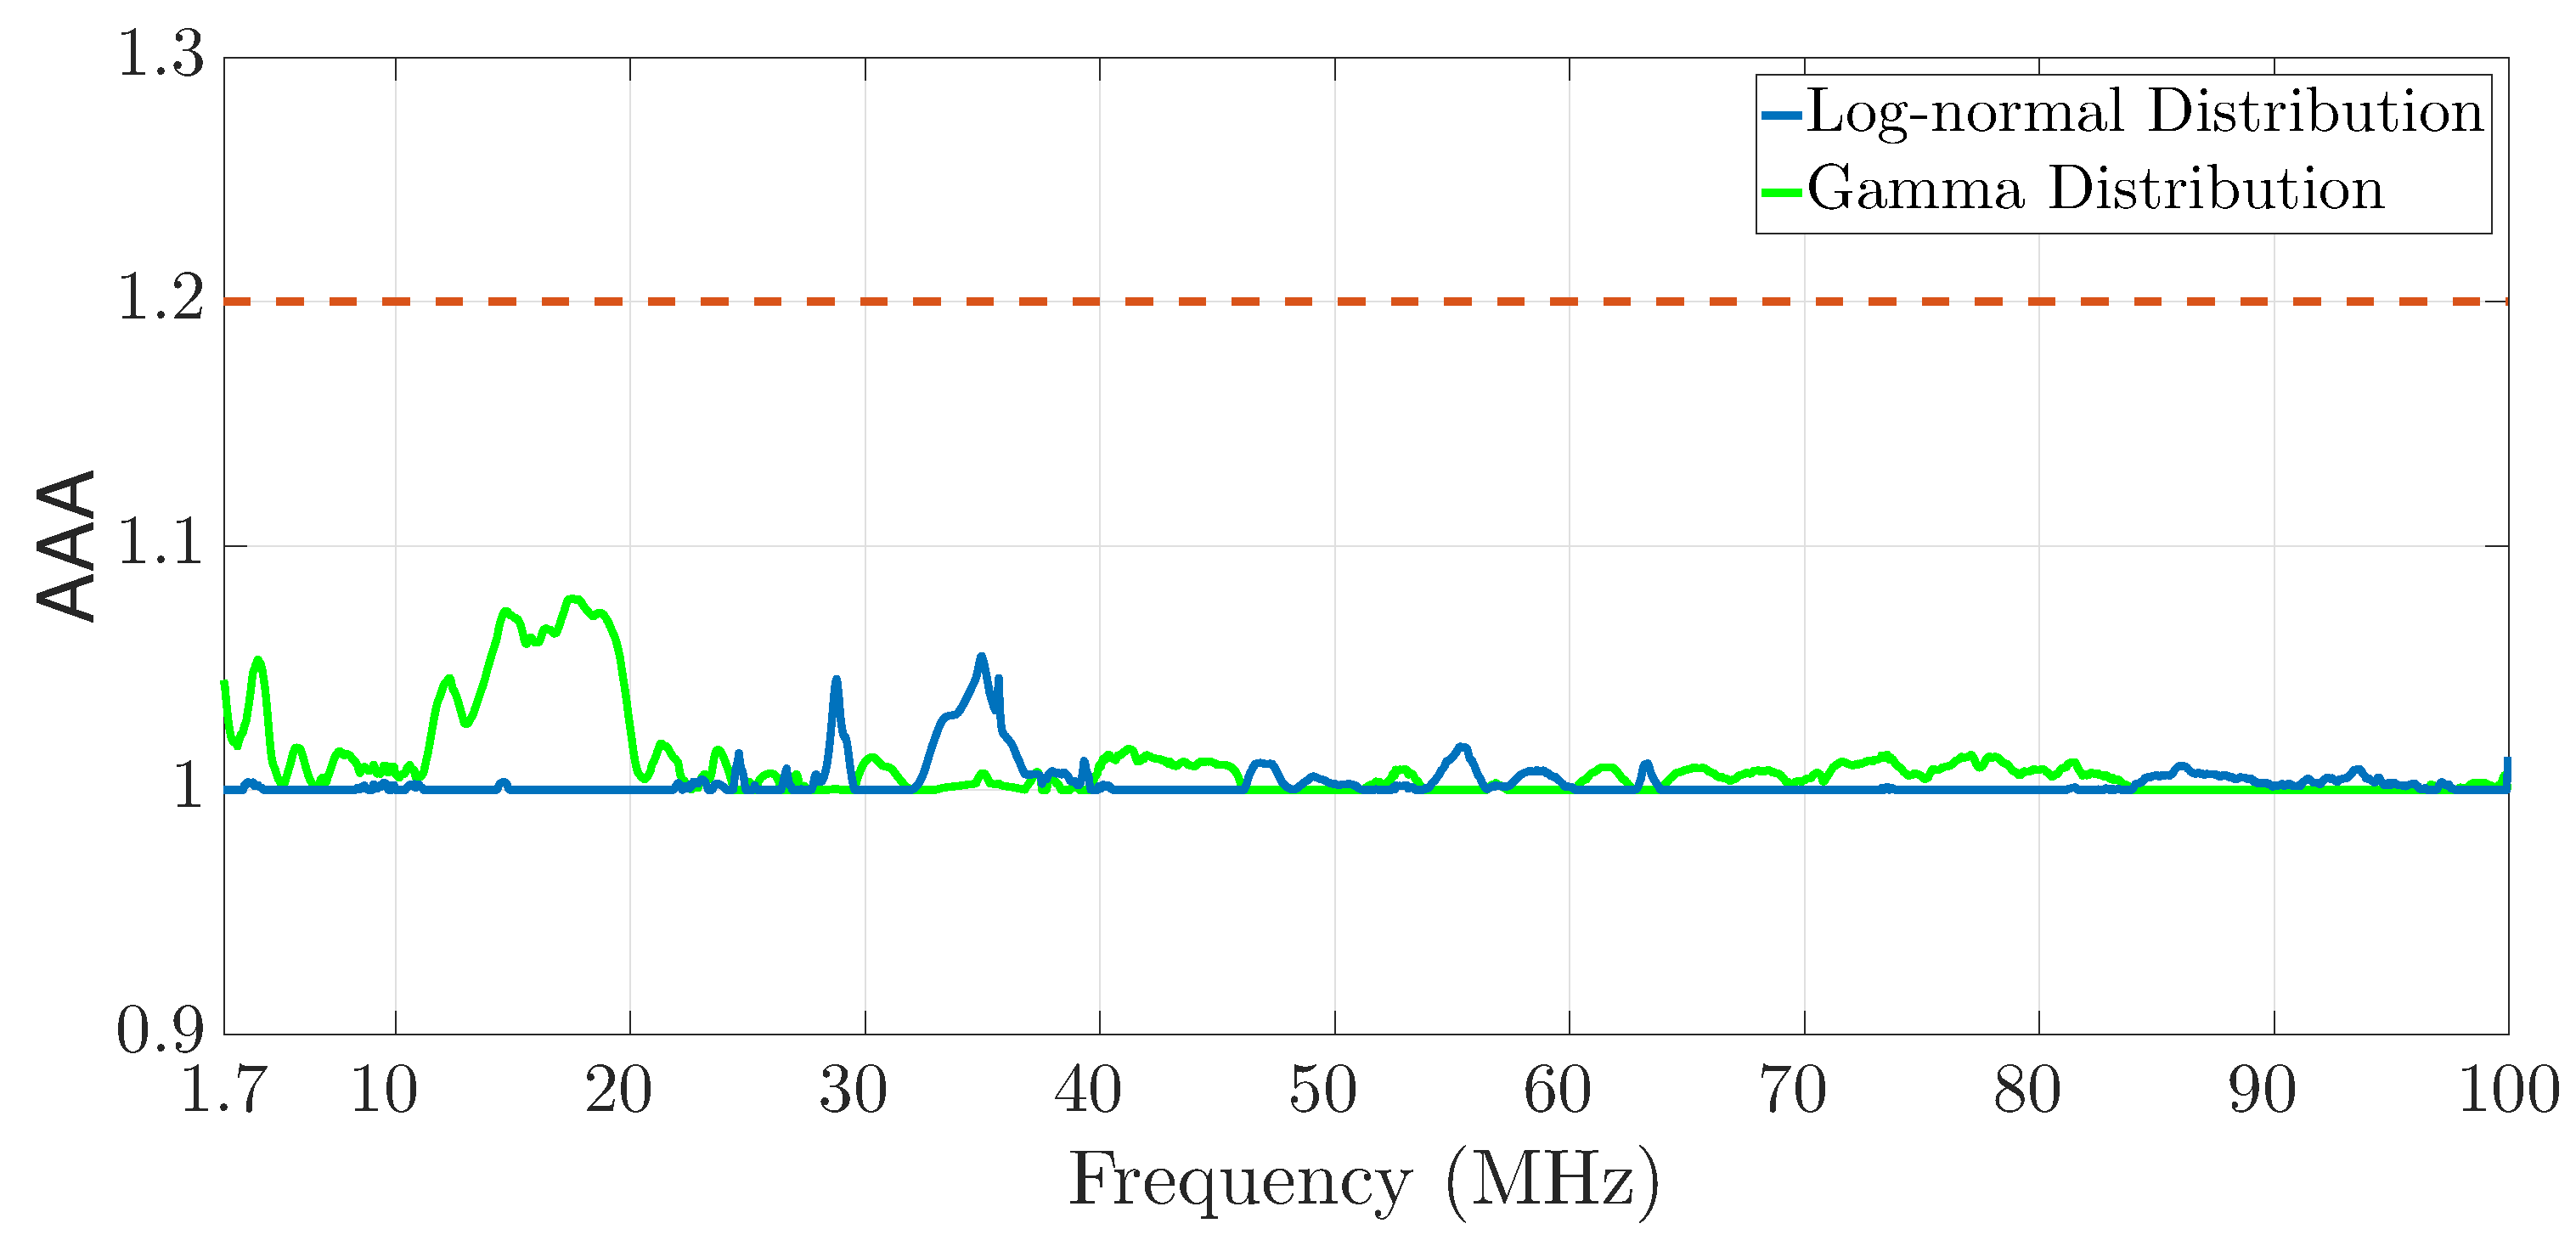
\includegraphics[width=0.49\textwidth]{images/Log_Lognormal_GammasW.eps}
	\caption{The values of $\rho_{A} (f)$ for the Log-normal and Gamma distributions.}
	\label{fig:Log_likesW}
\end{figure}


The statistical analysis of the magnitude of the valid \ac{PLC}-\ac{WLC} \textit{short-path} \ac{CFR} estimates showed that the parameters of the Log-normal distribution assume different values as frequency changes. If $\mathcal{C}_{|H_k|} = \{\alpha_1[k],\alpha_2[k]\}$ is the set of parameters for the statistical distribution modeling the magnitude of the valid \ac{CFR} estimates of \ac{PLC}-\ac{WLC} \textit{short-path} channels, where $k=0,1,\cdots,N-1$,  $\alpha_1[k] = \mu[k]$ and $\alpha_2[k] = \sigma[k]$, are the two parameters ($U=2$) of the Log-normal distribution, named mean and standard deviation, respectively, associated with the $k$-th sample of the valid \ac{CFR}. Then, Fig. \ref{mag_examplesW} and Fig. \ref{mag_example2sW} show the statistical models for two different values of frequency: $f=50.78$~MHz ($k=1040 \rightarrow f = 1040\Delta f$) and $f=80.57$~MHz ($k=1650 \rightarrow f = 1650\Delta f$), respectively. The parameters of the Log-normal distribution are  $\mu(1040 \Delta f) = \alpha_1[1040]=-4.0117$ and $\sigma( 1040 \Delta f) = \alpha_2[1040] = 0.5903$; $\mu(1650 \Delta f) = \alpha_1[1650] = -5.034$ and $\sigma( 1650 \Delta f) = \alpha_2[1650]=0.82$ for $f=50.78$~MHz and $f=80.57$~MHz, respectively.

\begin{figure}[h!]
	\centering
	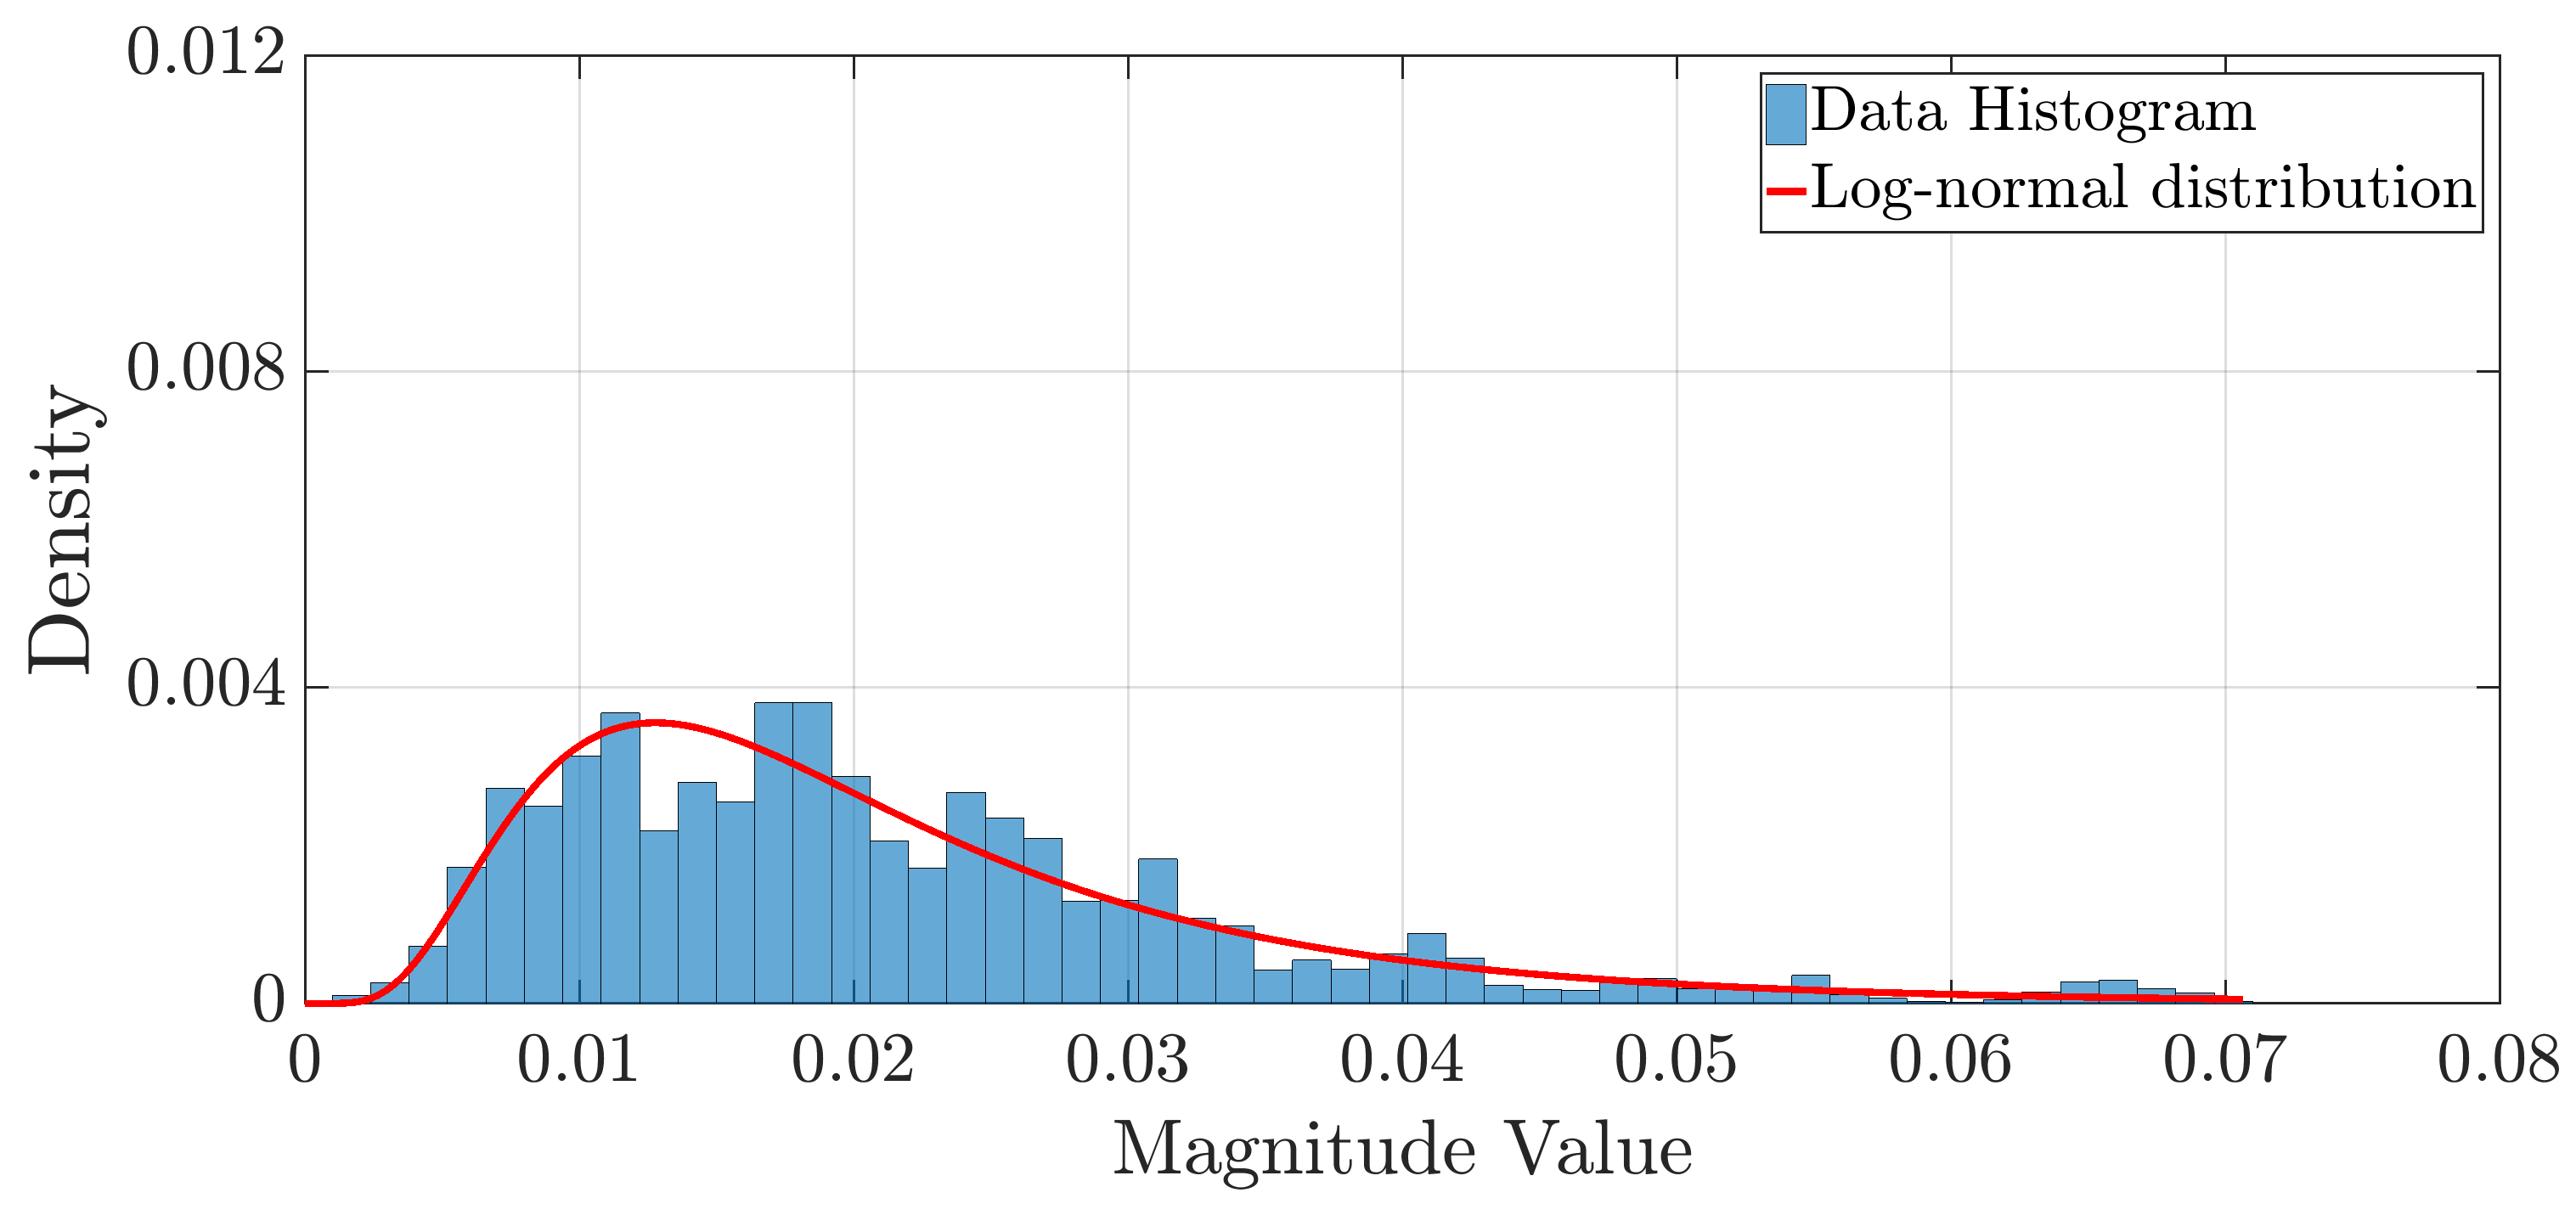
\includegraphics[width=0.49\textwidth]{images/Mag_histsW_2.eps}
	\caption{The relative frequency of the magnitude of the valid CFR estimates at the sample $k = 1040$ ($k\Delta f= 50.78$~MHz) and the modeling based on the Log-normal distribution.}
	\label{mag_examplesW}
\end{figure}

\begin{figure}[h!]
	\centering
	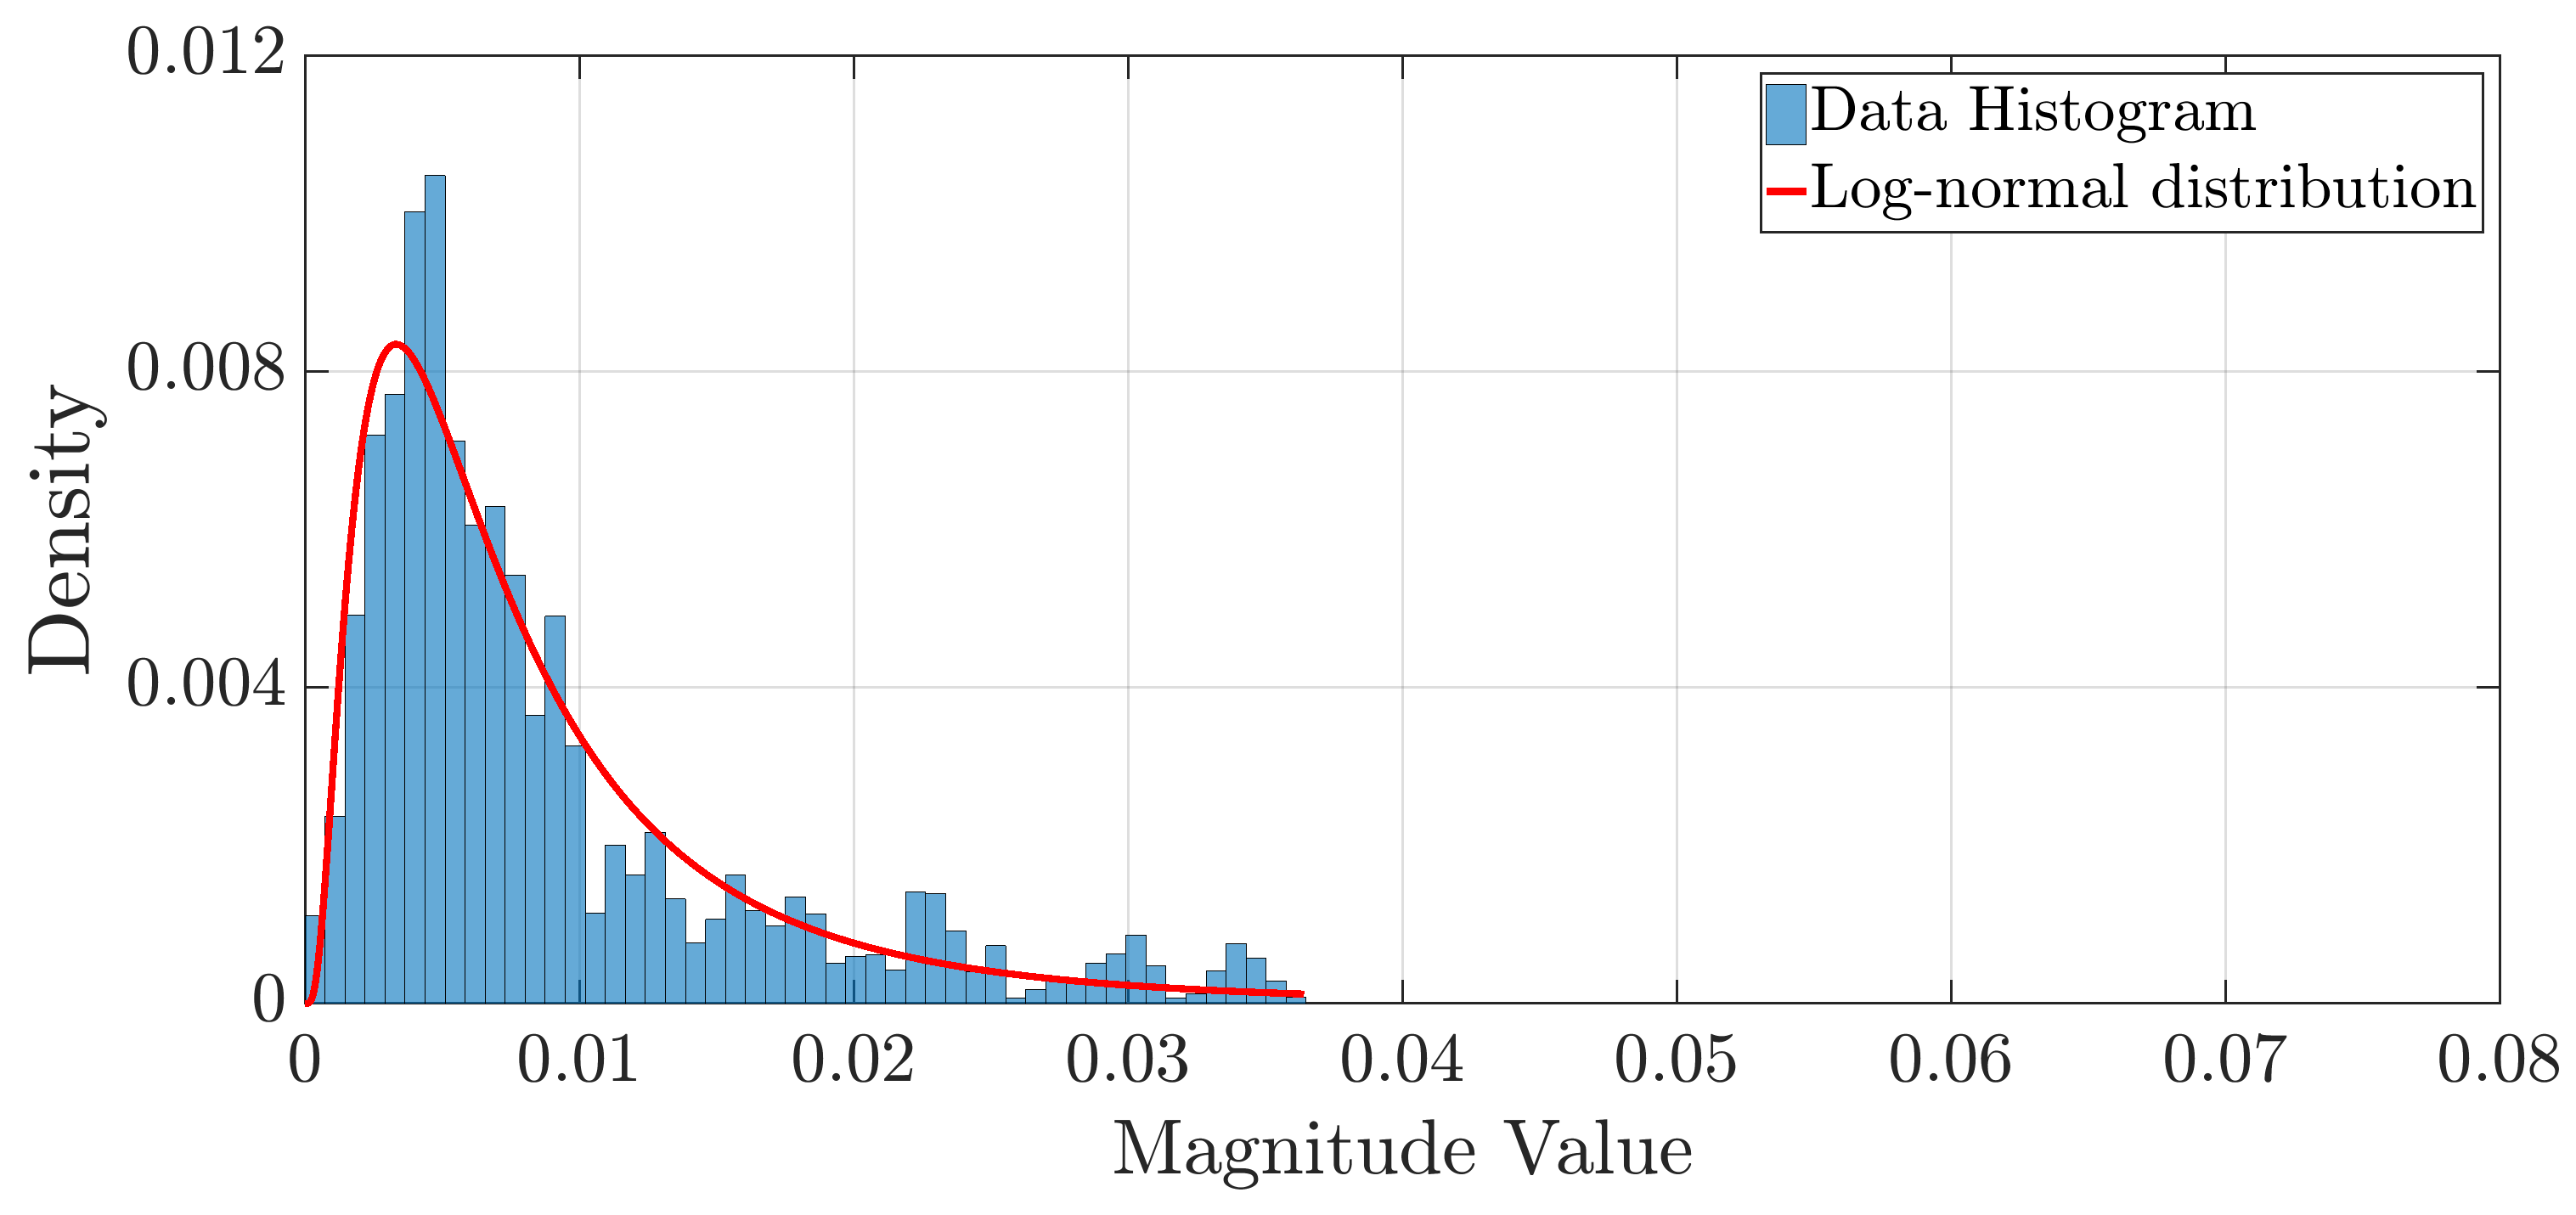
\includegraphics[width=0.49\textwidth]{images/Mag_hist2sW_2.eps}
	\caption{ The relative frequency of the magnitude of the valid CFR estimates at the sample $k = 1650$ ($k\Delta f= 80.57$~MHz) and the modeling based on the Log-normal distribution.}
	\label{mag_example2sW}
\end{figure}

By interpolating the parameters values $\mu[k]$ and $\sigma[k]$ of the Log-normal distributions associated with the model of the \ac{CFR} of the hybrid \ac{PLC}-\ac{WLC} \textit{short-path} channel using $L=15$ subbands, the continuous curves of parameters $\hat{\mu}(\omega)$ and $\hat{\sigma}(\omega)$ are yielded. Finally, the curves $\hat{\mu}(f)$ and $\hat{\sigma}(f)$ are easily obtained once $\omega \in [0,\pi)$ directly corresponds to the frequency band between $0$ and $100$~MHz. Figs. \ref{Fit_alfasW} and \ref{Fit_betasW} show the curves for the parameters $\mu(f)$ and $\sigma(f)$, which are obtained by applying frequency domain interpolation technique detailed in \cite{mitra} and the curves obtained by using the cubic Spline interpolation with $L=15$ subbands. Similar to the previous subsection, Table \ref{table_alfasW} lists the cubic Spline coefficients for modeling the parameter $\mu(f)$, of the valid \ac{CFR} magnitude while Table \ref{table_betasW}, covers the cubic Spline coefficients for modeling the parameter $\sigma(f)$. Overall, it is important to point out that the Log-normal distribution and its coefficients waveform $\hat{\mu(f)}$ and $\hat{\sigma(f)}$ define the random process representing the magnitude of the \acp{CFR} of the in-home hybrid \ac{PLC}-\ac{WLC} \textit{short-path} channel.

\begin{figure}[h]
	\centering
	\psfrag{Interval Boundsaa}[c][c][0.7]{Interval Bounds}
	\psfrag{AAA}[c][c][0.7]{$~~~~~\mu(k \Delta f)$}
	\psfrag{BBB}[c][c][0.7]{$~\hat{\mu}(f)$}
	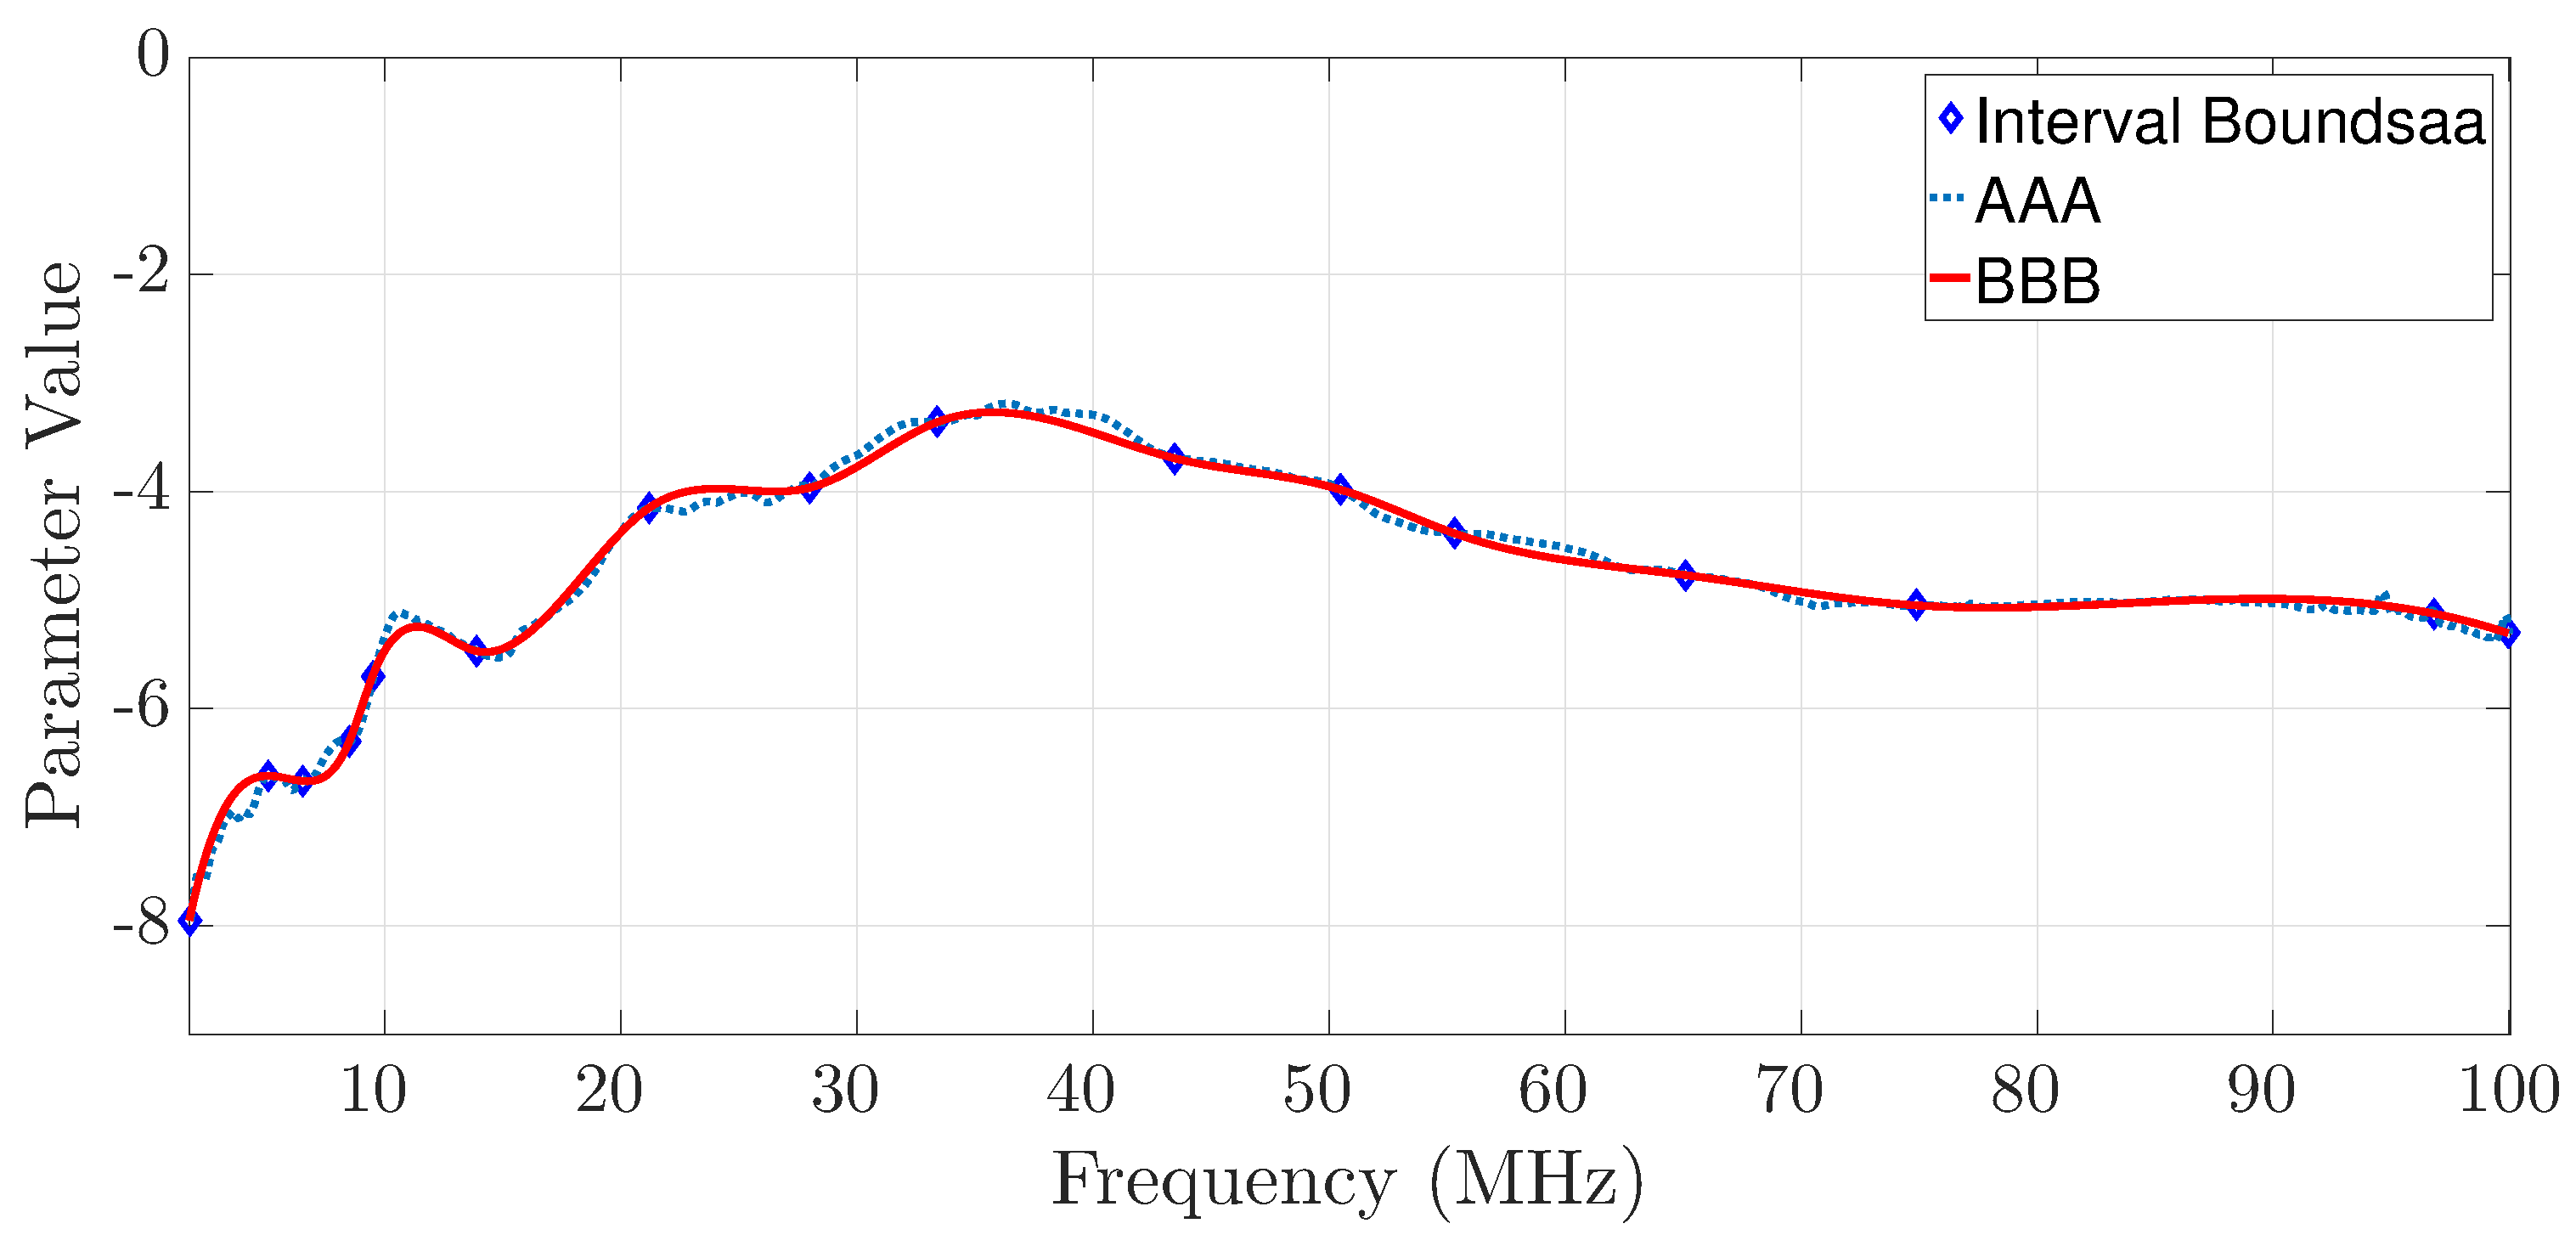
\includegraphics[width=0.49\textwidth]{images/Alfa_fitsW.eps}
	\caption{The result of the interpolation technique based on cubic Splines applied to obtain $\mu(f)=\zeta_1(f)$ for the Log-normal distribution (${\mu}(k \Delta f)$ are the original values of the parameter and $\hat{\mu}(f)$ is the interpolated curve).}
	\label{Fit_alfasW}
\end{figure}

\begin{figure}[h]
	\centering
	\psfrag{Interval Boundsaa}[c][c][0.7]{Interval Bounds}
	\psfrag{AAA}[c][c][0.7]{${~~~~~\sigma}(k \Delta f)$}
	\psfrag{BBB}[c][c][0.7]{$~\hat{\sigma}(f)$}
	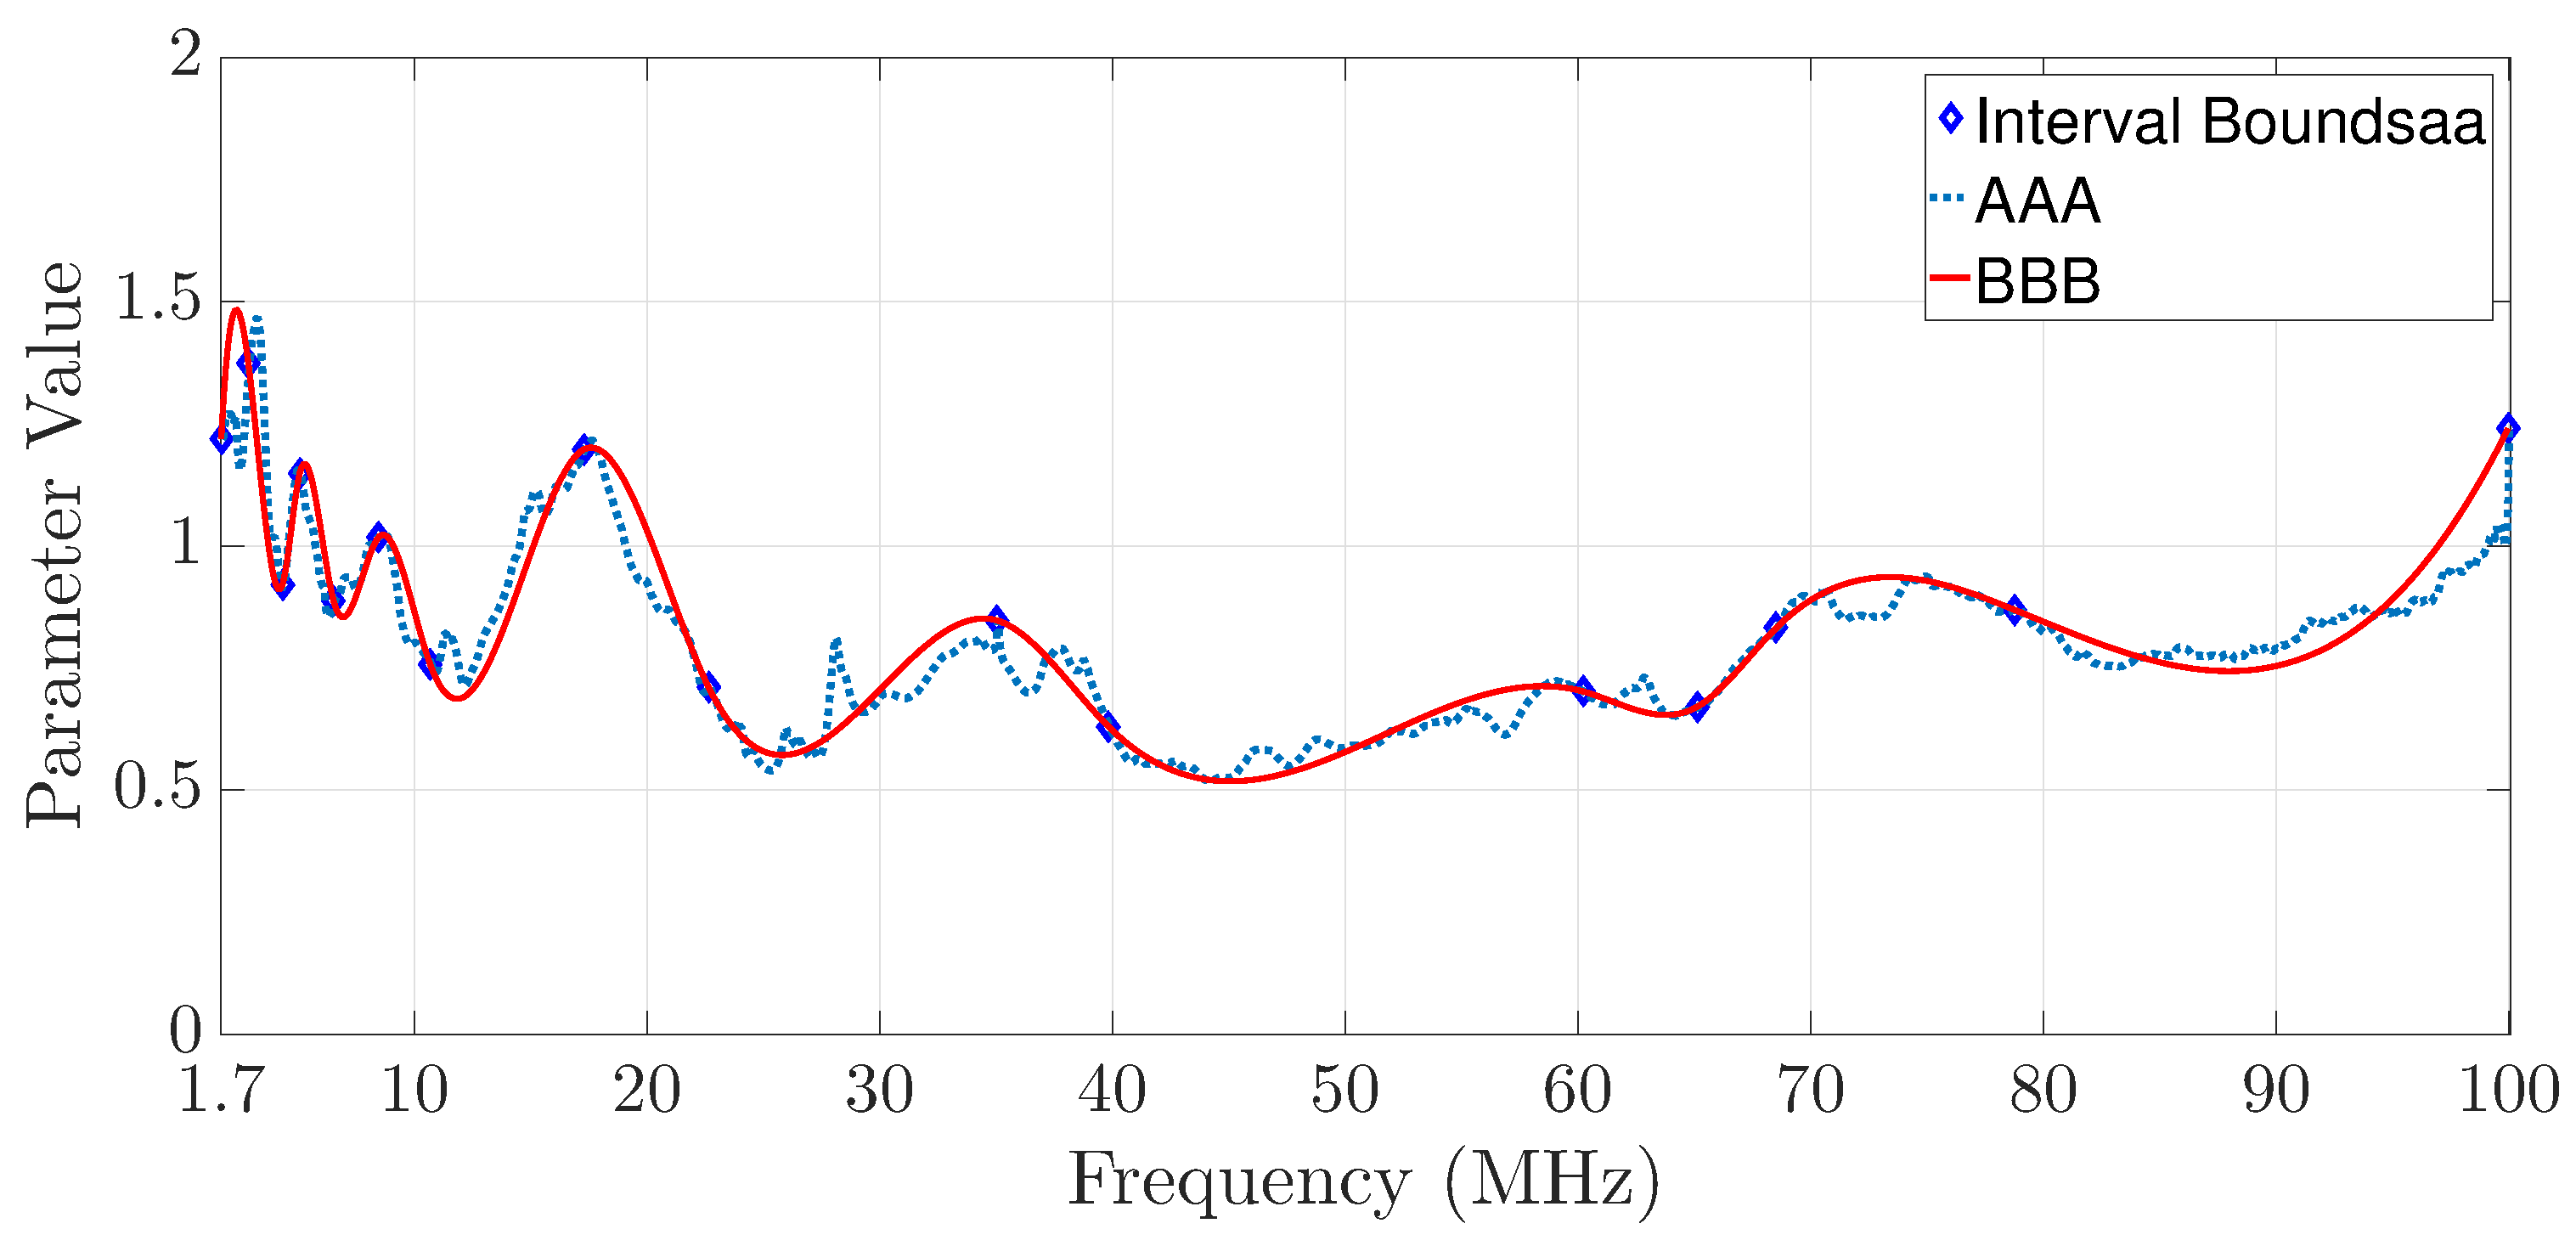
\includegraphics[width=0.49\textwidth]{images/Beta_fitsW.eps}
	\caption{The result of the interpolation technique based on cubic Splines applied to obtain $\sigma(f)=\zeta_2(f)$ for the Log-normal distribution (${\sigma}(k \Delta f)$ are the original values of the parameter and $\hat{\sigma}(f)$ is the interpolated curve).}
	\label{Fit_betasW}
\end{figure}

\subsection{Hybrid PLC-WLC long-path channels}\label{sec:MMHYBL}

For illustration purposes, Fig. \ref{respfreqlW} shows five valid and consecutive estimates of the \ac{CFR} magnitude. On this scenario the average operation was not used on the \ac{CFR} estimates, since the coherence time of the \ac{PLC}-\ac{WLC} \textit{long-path} channels was not long enough to contain the duration of at least two symbol periods ($T_{\textrm{sym}}$). Note that the channel attenuation ranges from approximately $-45$~dB up to -$15$~dB and the plots cover a time interval equal to $\Delta T_{\textrm{sym}}\approx23.04~\mu$s and, as a consequence, $5\Delta T = 115.2~\mu$s.

\begin{figure}[h]
	\centering
	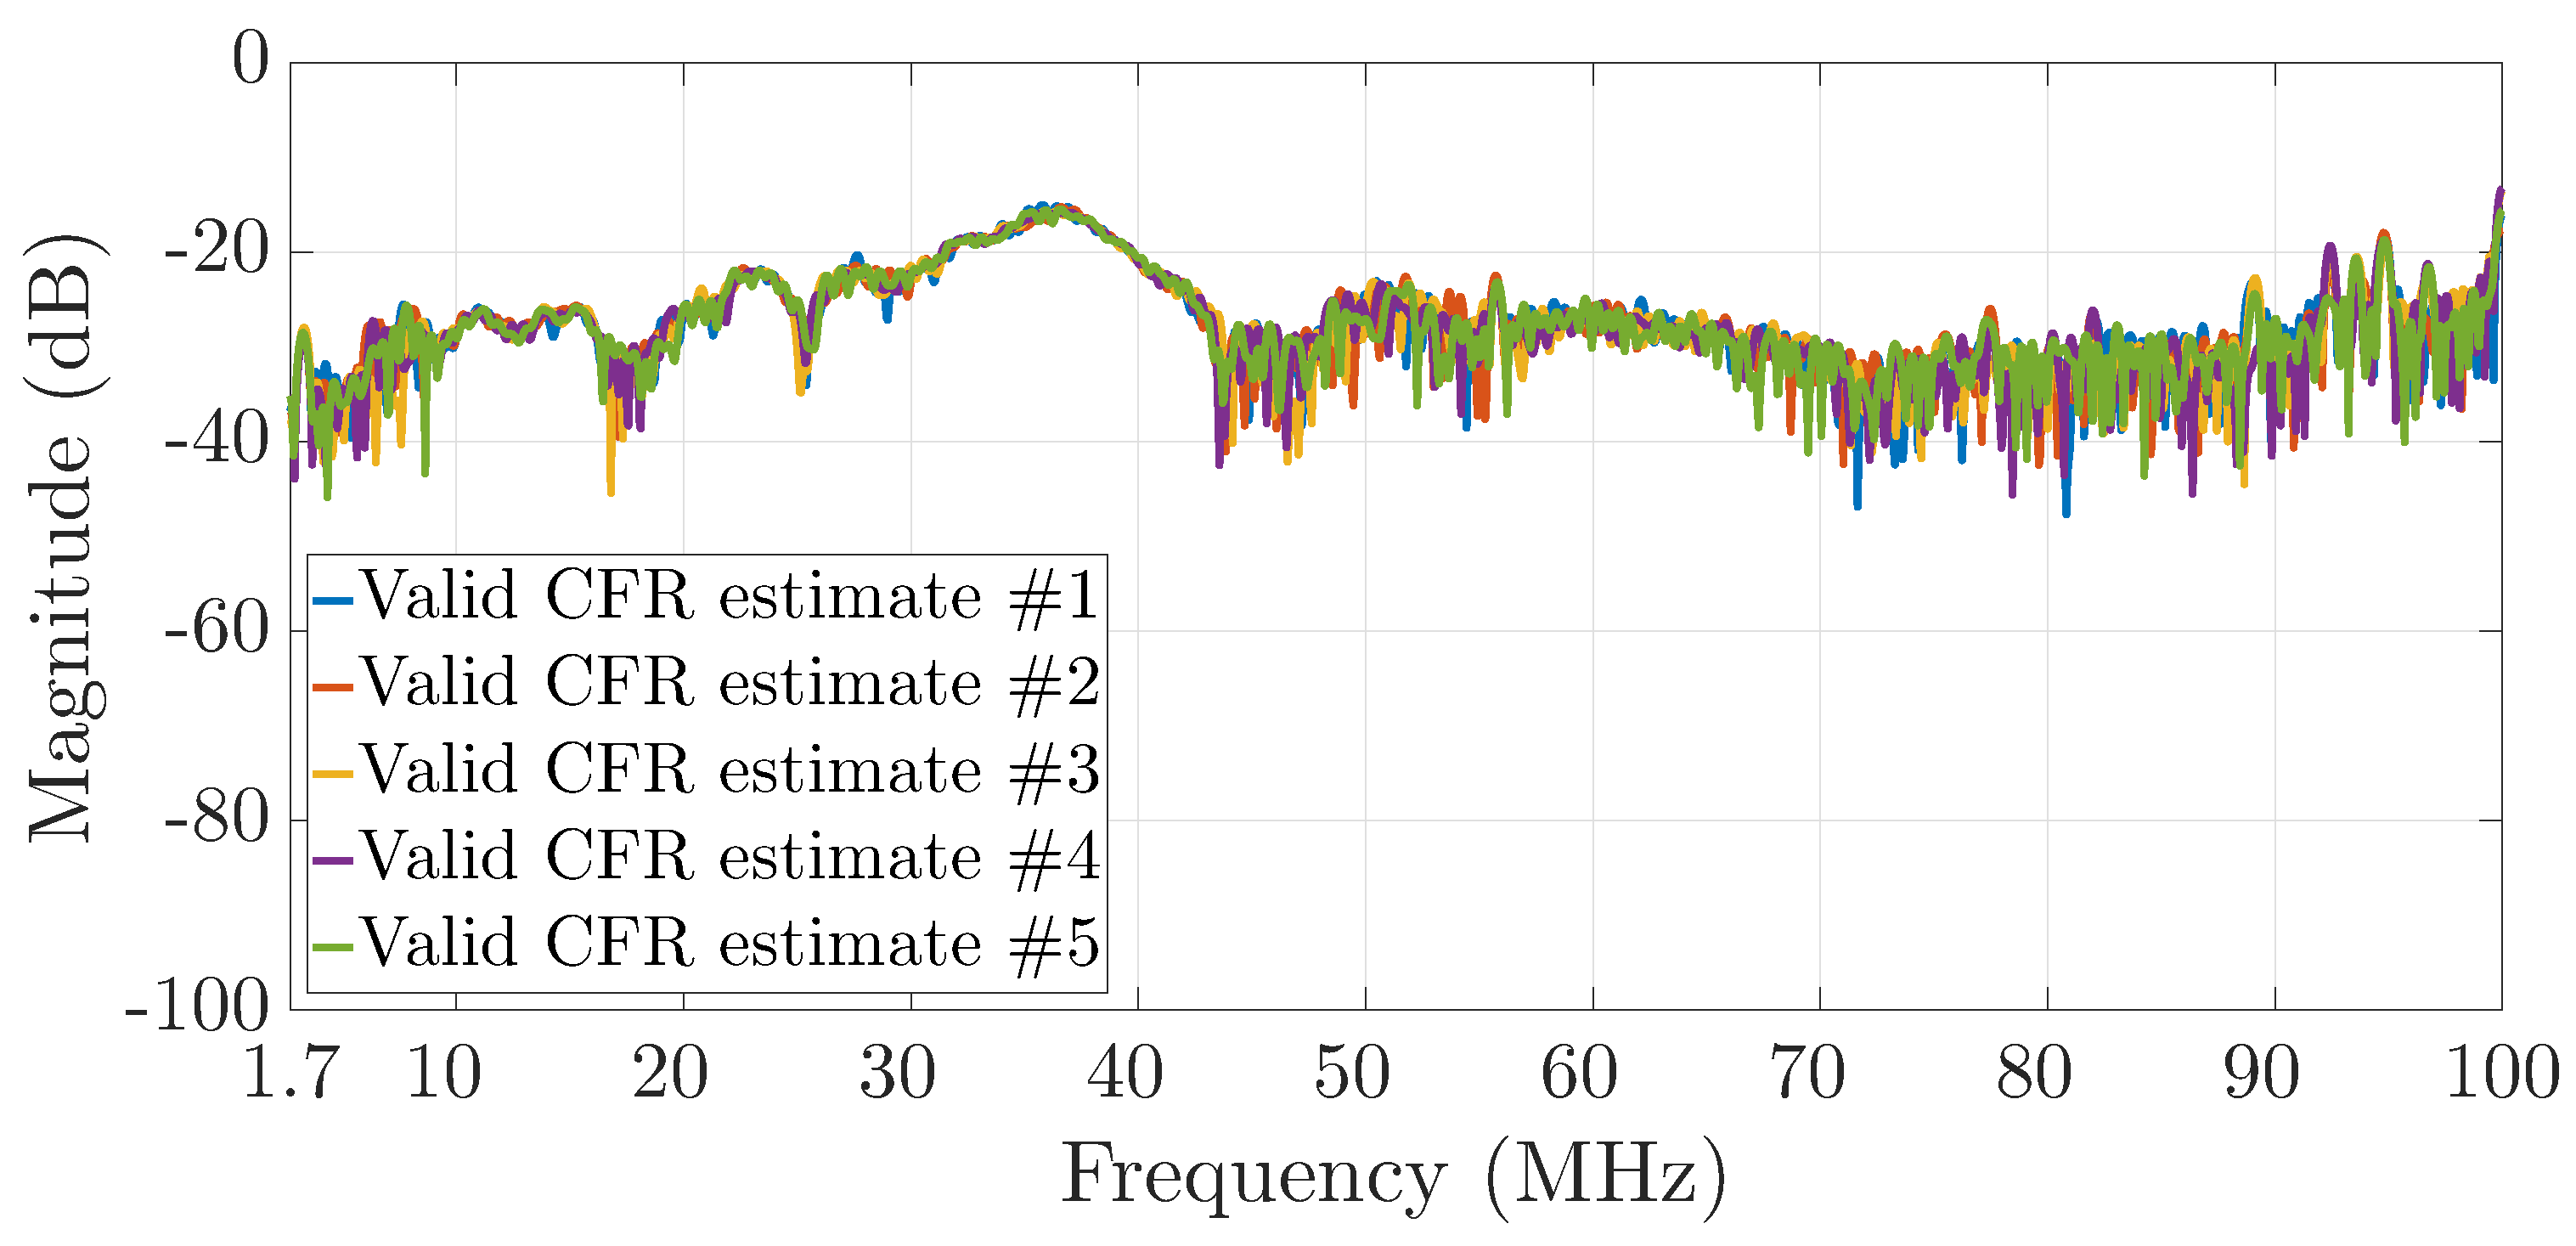
\includegraphics[width=0.49\textwidth]{images/respfreqlW.eps}
	\caption{Five consecutive and valid CFR magnitudes of the measured in-home PLC-WLC \textit{long-path} channel.}
	\label{respfreqlW}
\end{figure}

Fig. \ref{MAG_percentlW} shows the relative frequency of statistical distributions that had modeled, in accord with the adopted criteria, the magnitude of the whole set of valid \ac{CFR} estimates. Similarly to the results acquired on the \ac{PLC}-\ac{WLC} \textit{short-path} channels, a single statistical distribution has modeled the majority of the magnitudes, but another different statistical distribution stood out as possible candidate to model the \ac{CFR} magnitudes. As a matter of fact, in 51\% of the \ac{CFR} estimates the Log-normal distribution resulted in the best model and in 38\% of it the Gamma distribution offered the best modeling. 

\begin{figure}[h!]
	\centering
	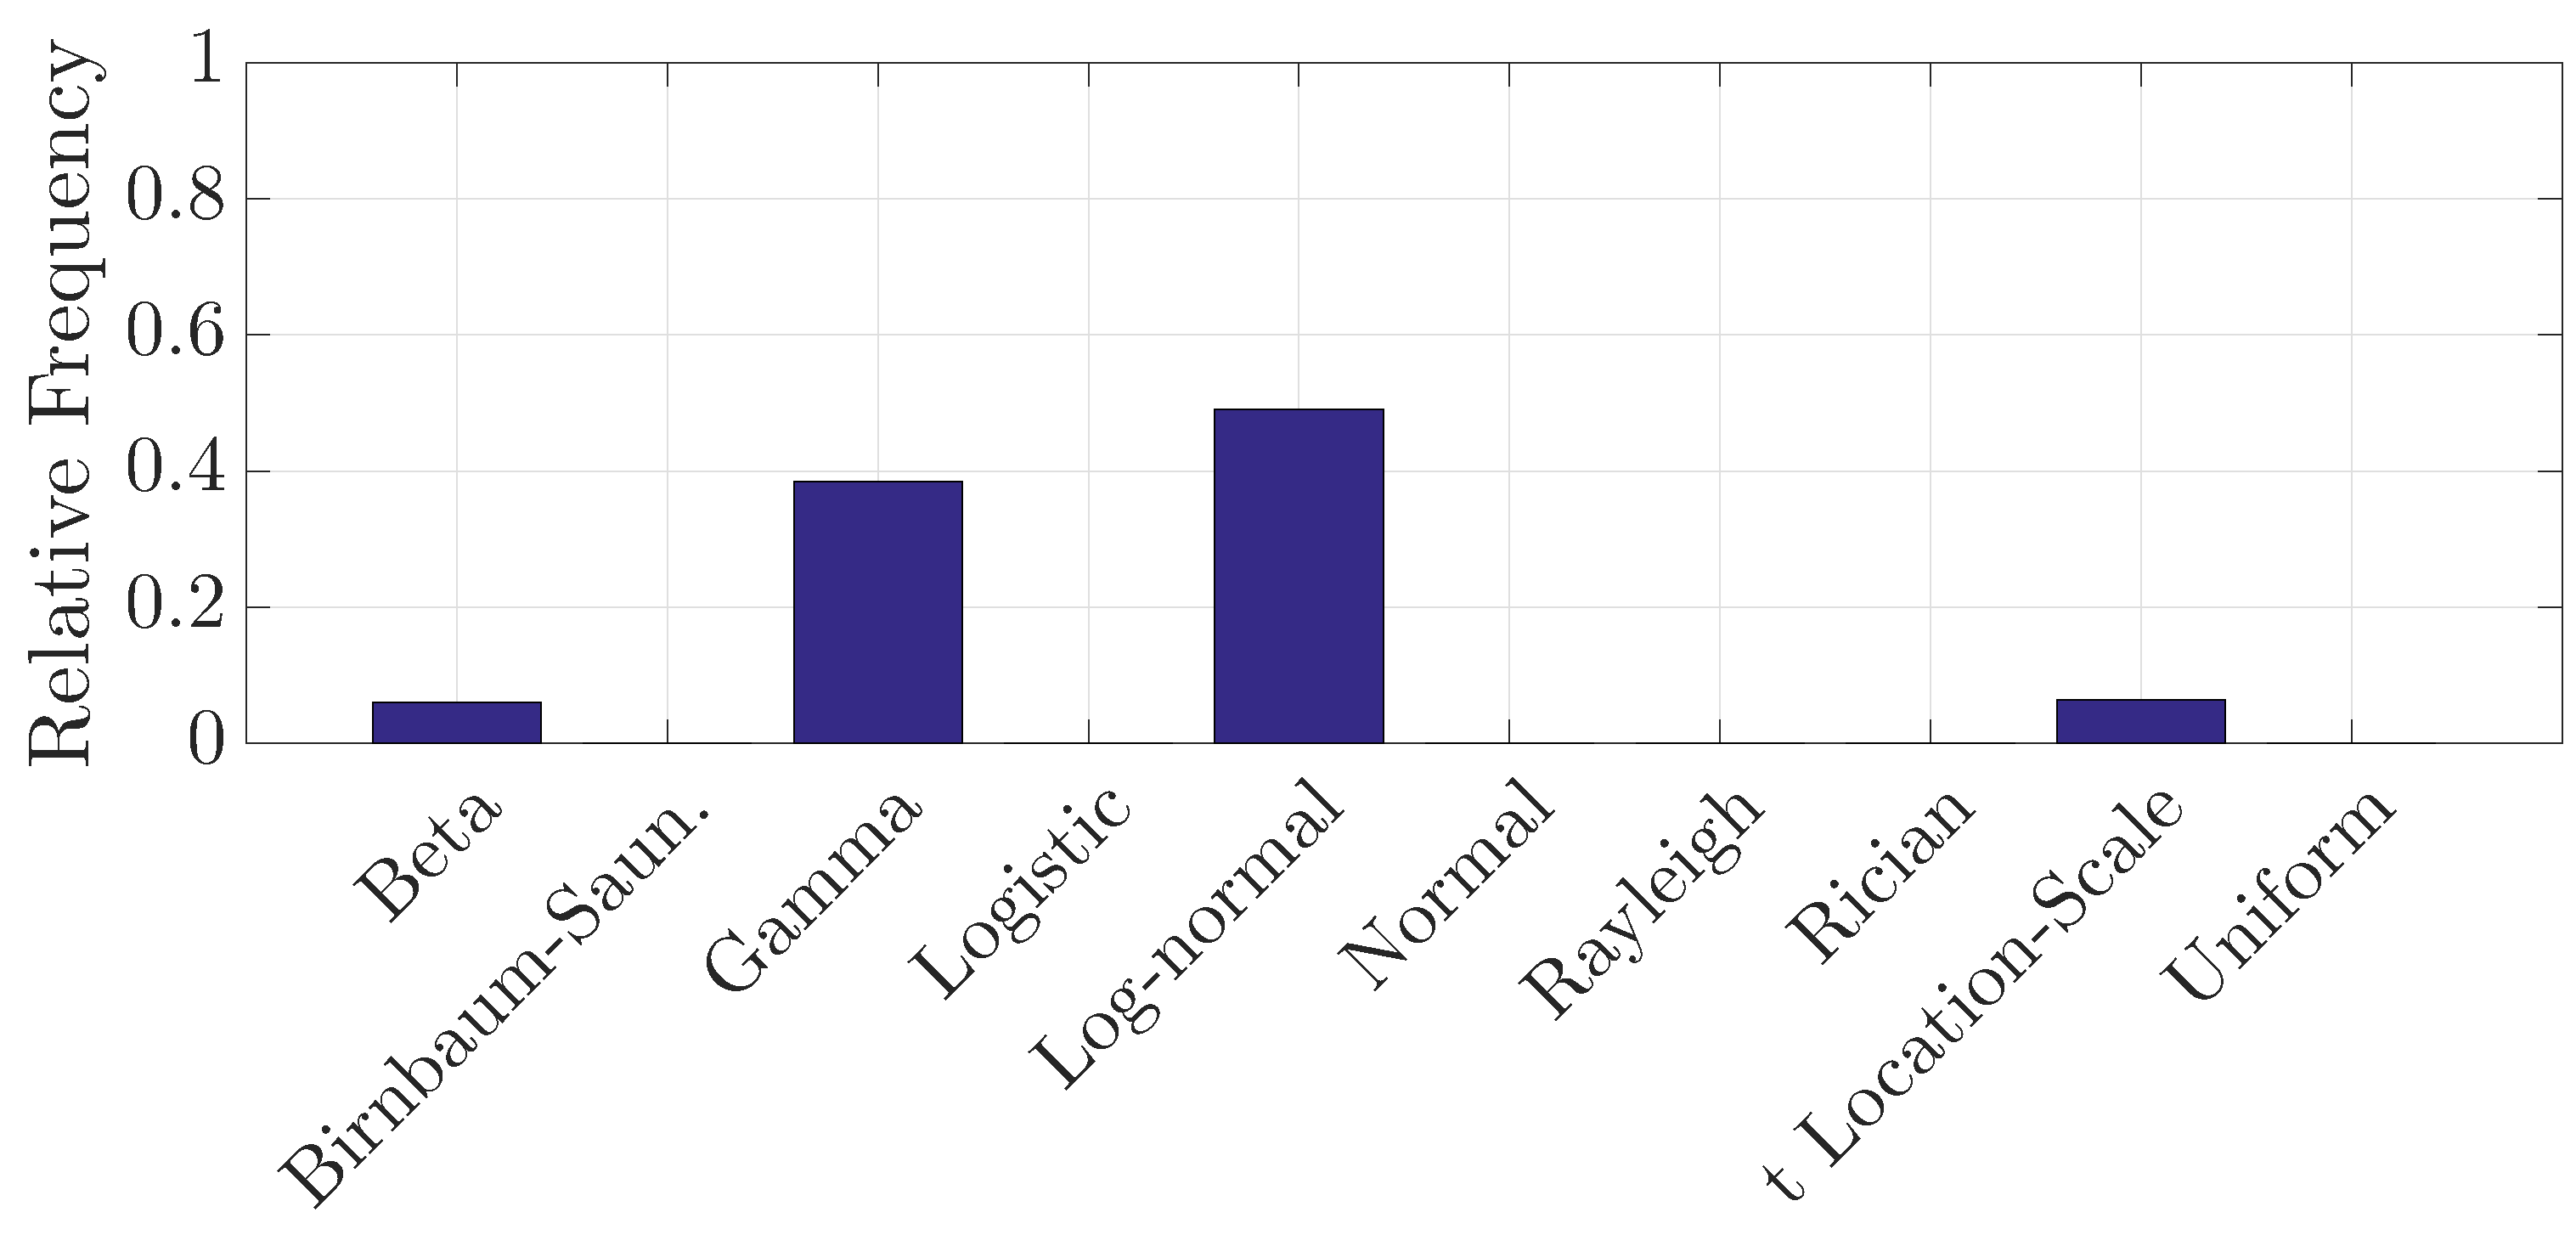
\includegraphics[width=0.49\textwidth]{images/Mag_percentlW.eps}
	\caption{The relative frequency associated with the chosen statistical distribution that best models the CFR magnitude in accord with the adopted criteria.}
	\label{MAG_percentlW}
\end{figure}

Once again (\ref{eq:log-lik}) was used in order to evaluate which of the two distributions is the best choice to model the magnitude component of the \ac{CFR} estimates. Fig. \ref{fig:Log_likelW} portrays the values of  $\rho_A}(f)$ for the two best statistical distributions candidates to model the magnitude of the valid \ac{CFR} estimates. These curves emphasize that only the Log-normal distributions achieved the minimum ratio over the \ac{MLE} criterion. Overall, the results in Fig. \ref{MAG_percentlW} and Fig. \ref{fig:Log_likelW} illustrates that the Log-normal distribution is the best option to model the magnitude of the valid \ac{CFR} estimates of the measured in-home hybrid \ac{PLC}-\ac{WLC} \textit{long-path} channels. In other words, the magnitude of the valid \ac{CFR} estimates of in-home hybrid \ac{PLC}-\ac{WLC} \textit{long-path} channels can be modeled by using only one statistical distribution (i.e., the Log-normal distribution).

\begin{figure}[h!]
	\centering
	\psfrag{AAA}[c][c][1.0]{$\rho_{A} (f)$}
	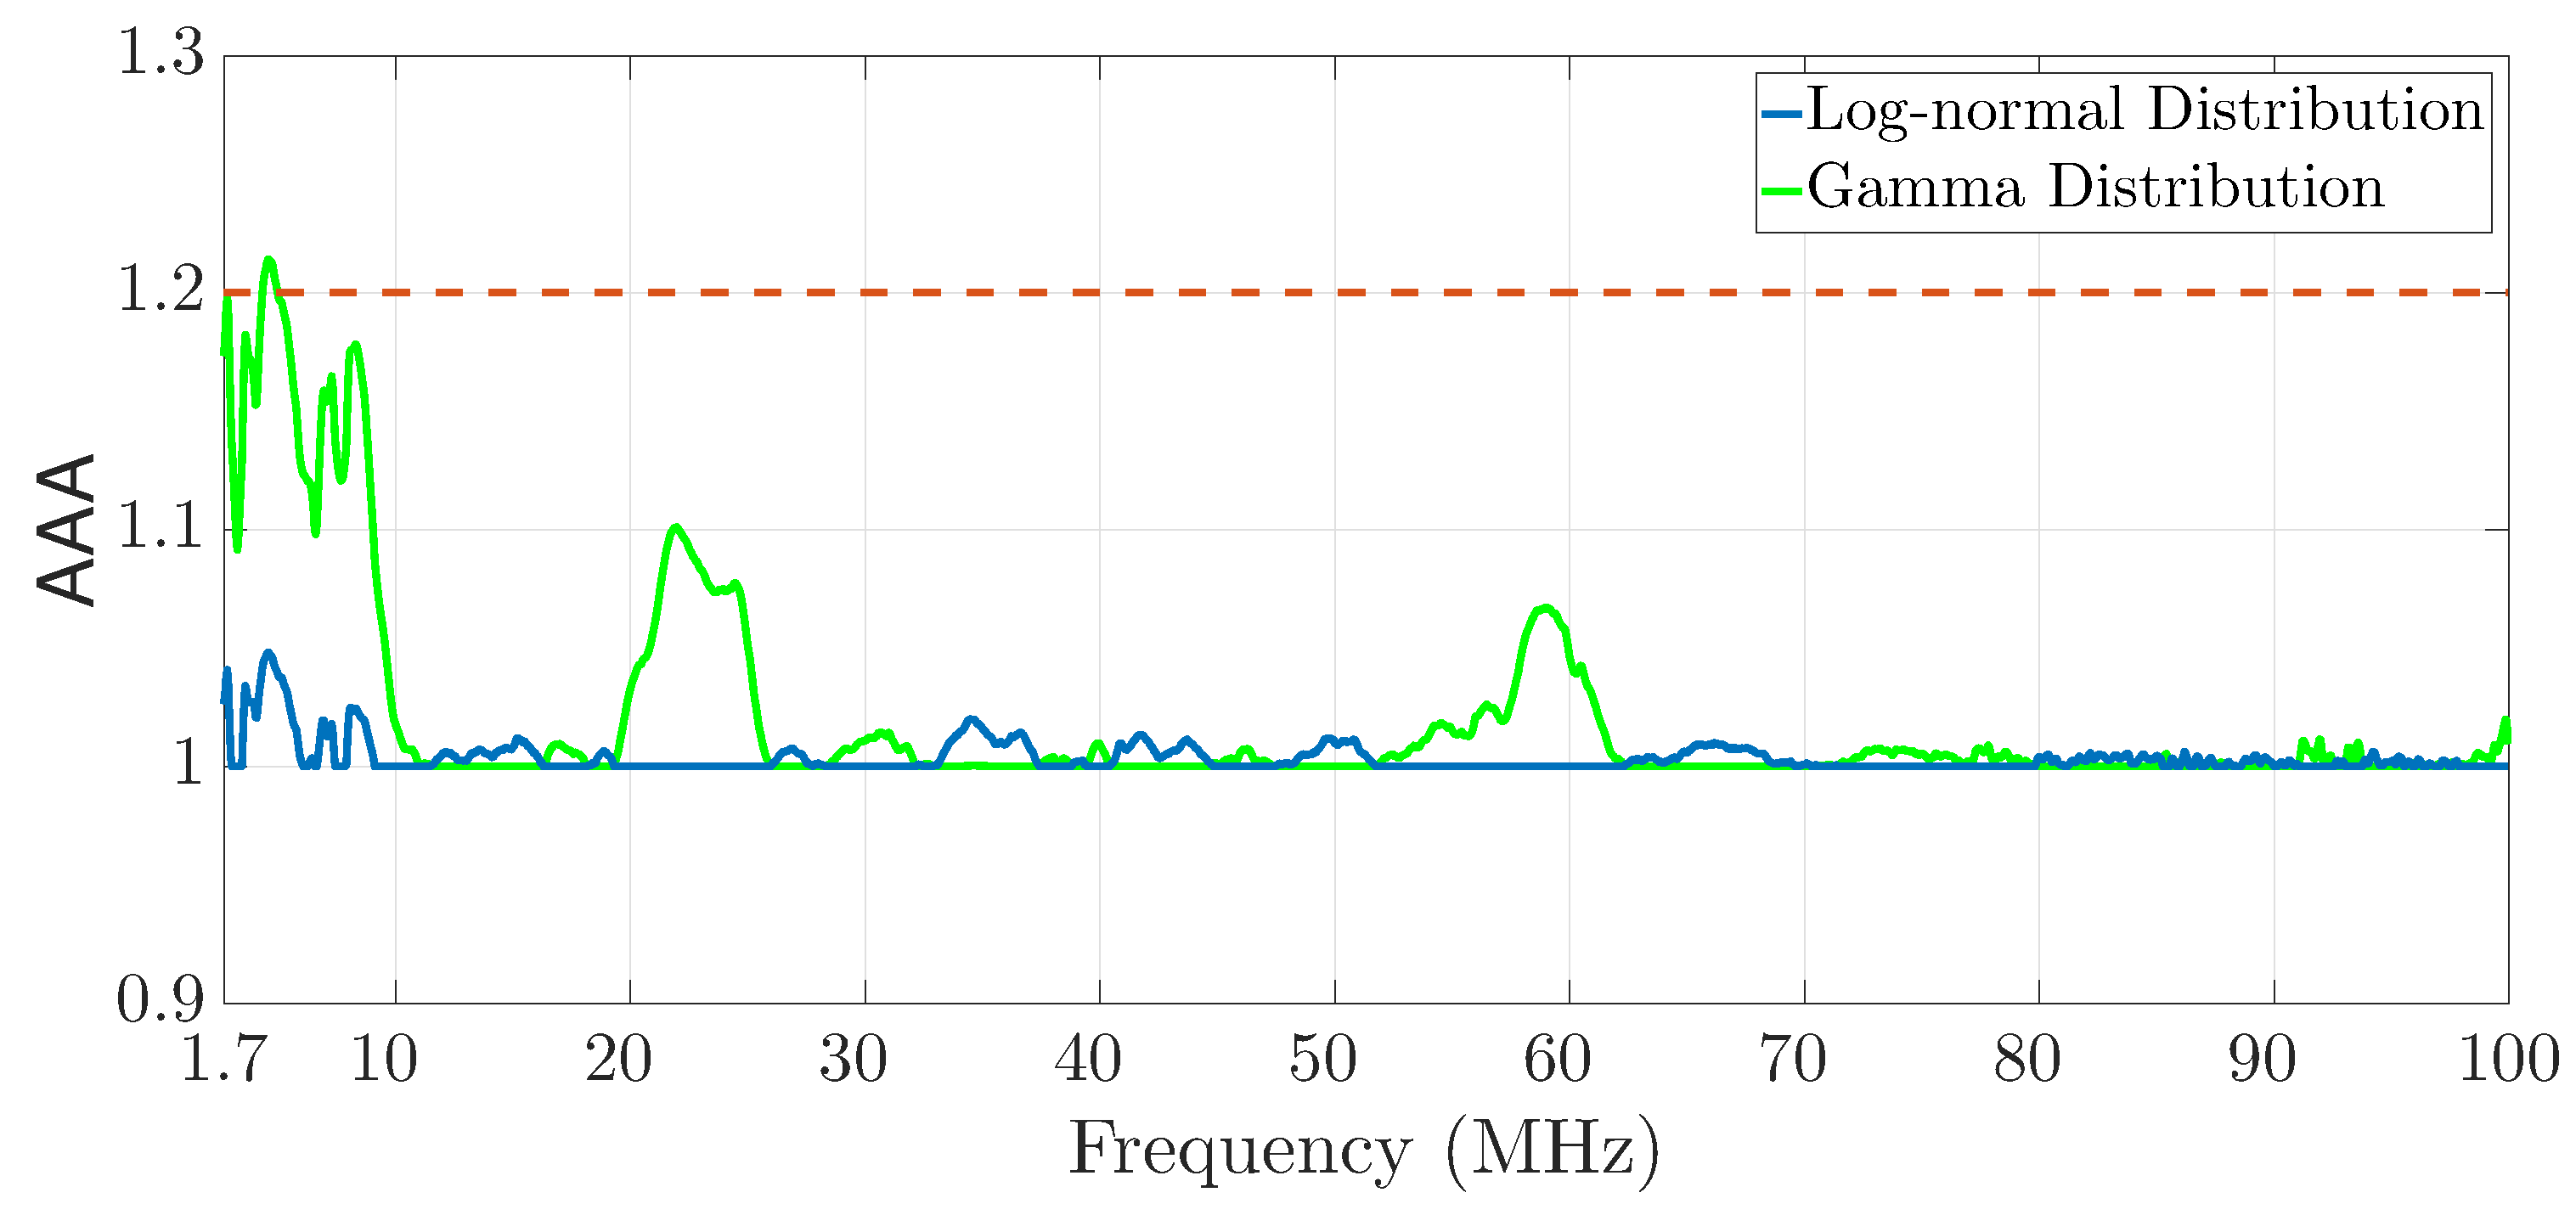
\includegraphics[width=0.49\textwidth]{images/Log_Lognormal_GammalW.eps}
	\caption{The values of $\rho_{A} (f)$ for the Log-normal and Gamma distributions.}
	\label{fig:Log_likelW}
\end{figure}

The statistical analysis of the magnitude of the valid \ac{CFR} estimates shows that the parameters of the Log-normal distribution assume different values as frequency changes. If $\mathcal{C}_{|H_k|} = \{\alpha_1[k],\alpha_2[k]\}$ is the set of parameters for the statistical distribution modeling the magnitude of the valid \ac{CFR} estimates of \ac{PLC}-\ac{WLC} \textit{short-path} channels, where $k=0,1,\cdots,N-1$,  $\alpha_1[k] = \mu[k]$ and $\alpha_2[k] = \sigma[k]$, are the two parameters ($U=2$) of the Log-normal distribution, named mean and standard deviation, respectively, associated with the $k$-th sample of the valid \ac{CFR}. Then, Fig. \ref{mag_examplelW} and Fig. \ref{mag_example2lW} show the statistical models for two different values of frequency: $f=51.76$~MHz ($k=1060 \rightarrow f = 1060\Delta f$) and $f=78.1$~MHz ($k=1600 \rightarrow f = 1600\Delta f$), respectively. The parameters of the Log-normal distribution are  $\mu(1060 \Delta f) = \alpha_1[1060]=-6.0759$ and $\sigma( 1060 \Delta f) = \alpha_2[1040] = 0.8118$; $\mu(1600 \Delta f) = \alpha_1[1600] = -6.8347$ and $\sigma( 1600 \Delta f) = \alpha_2[1600]=0.8407$ for $f=51.76$~MHz and $f=78.1$~MHz, respectively.

\begin{figure}[h!]
	\centering
	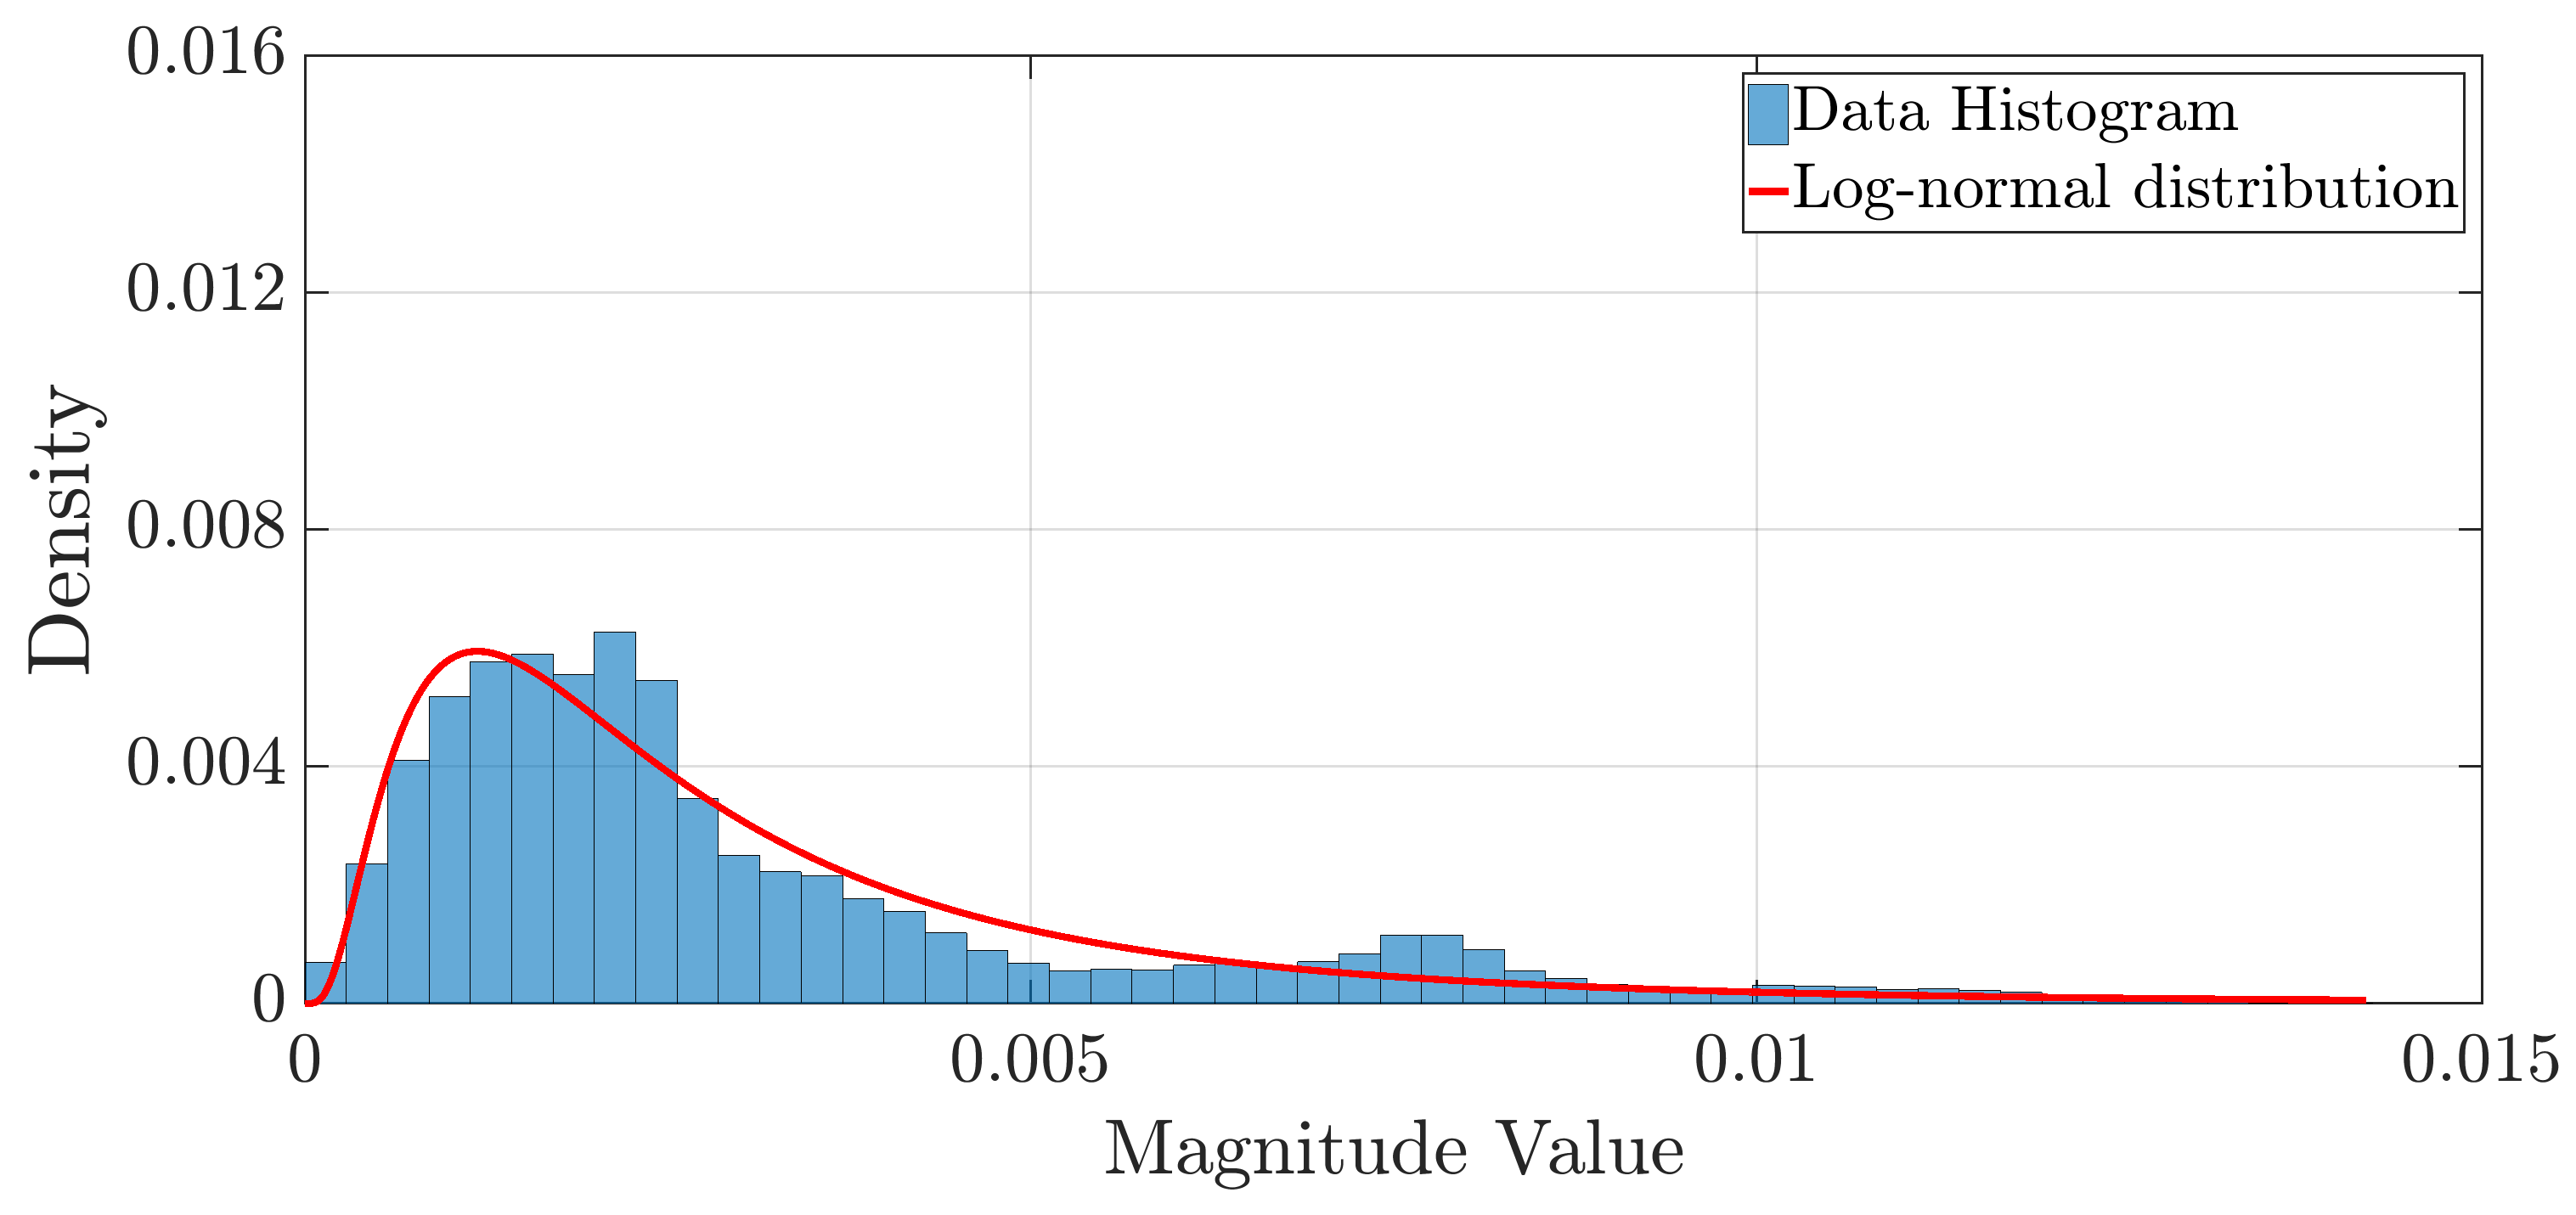
\includegraphics[width=0.49\textwidth]{images/Mag_histlW_2.eps}
	\caption{The relative frequency of the magnitude of the valid CFR estimates at the sample $k = 1060$ ($k\Delta f= 51.76$~MHz) and the modeling based on the Log-normal distribution.}
	\label{mag_examplelW}
\end{figure}

\begin{figure}[h!]
	\centering
	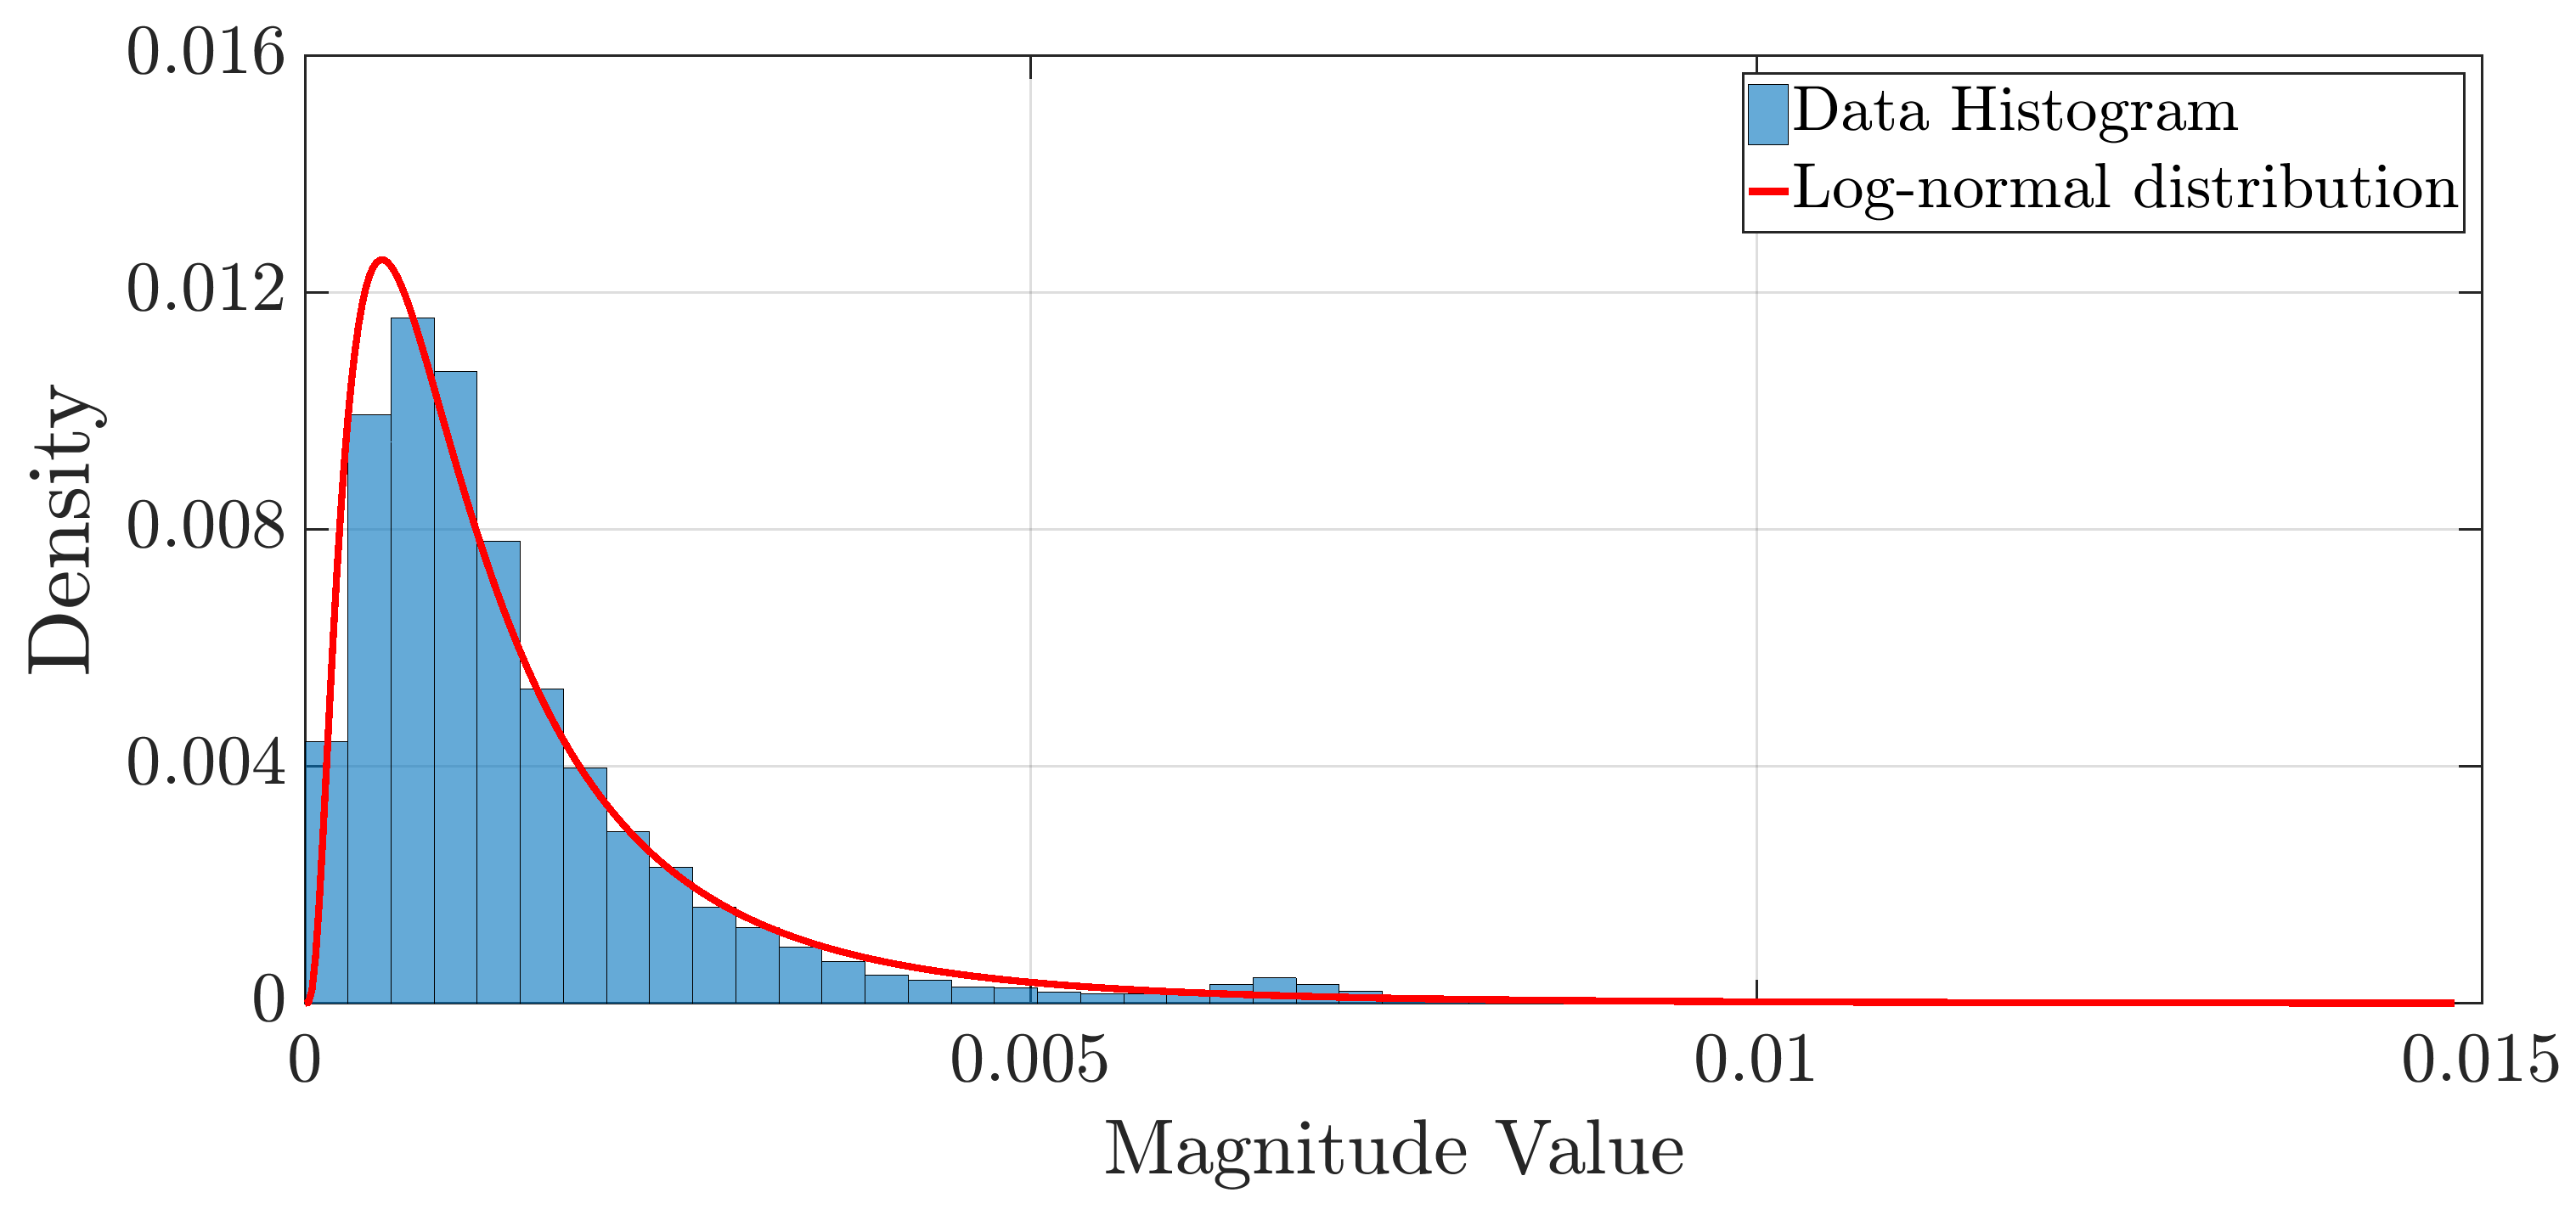
\includegraphics[width=0.49\textwidth]{images/Mag_hist2lW_2.eps}
	\caption{ The relative frequency of the magnitude of the valid CFR estimates at the sample $k = 1600$ ($k\Delta f= 78.1$~MHz) and the modeling based on the Log-normal distribution.}
	\label{mag_example2lW}
\end{figure}

Through the interpolation of the parameters values $\mu(k\Delta f)$ and $\sigma(k\Delta f)$ of the Log-normal distributions associated with the model of \ac{PLC}-\ac{WLC} \textit{long-path} \ac{CFR} using $L=15$ subbands, the continuous curves of parameters $\hat{\mu}(\omega)$ and $\hat{\sigma}(\omega)$ are yielded. Finally, the curves $\hat{\mu}(f)$ and $\hat{\sigma}(f)$ are easily obtained once $\omega \in [0,\pi)$ directly corresponds to the frequency band between $0$ and $100$~MHz. Figs. \ref{Fit_alfalW} and \ref{Fit_betalW} show the curves for the parameters $\mu(f)$ and $\sigma(f)$, which are obtained by applying frequency domain interpolation technique detailed in \cite{mitra} and the curves obtained by using the cubic Spline interpolation with $L=15$ subbands. Furthermore, Table \ref{table_alfalW} lists the cubic Spline coefficients for modeling the parameter $\mu(f)$, of the valid \ac{CFR} magnitude. Similarly, Table \ref{table_betalW} lists the cubic Spline coefficients for modeling the parameter $\sigma(f)$. As a result, the coefficients values, the waveforms  $\hat{\mu(f)}$ and $\hat{\sigma(f)}$, and the Log-normal distribution define the random process representing the magnitude of the \ac{CFR} of the in-home \ac{PLC}-\ac{WLC} \textit{long-path} channel.

\begin{figure}[h]
	\centering
	\psfrag{Interval Boundsaa}[c][c][0.7]{Interval Bounds}
	\psfrag{AAA}[c][c][0.7]{$~~~~~\mu(k \Delta f)$}
	\psfrag{BBB}[c][c][0.7]{$~\hat{\mu}(f)$}
	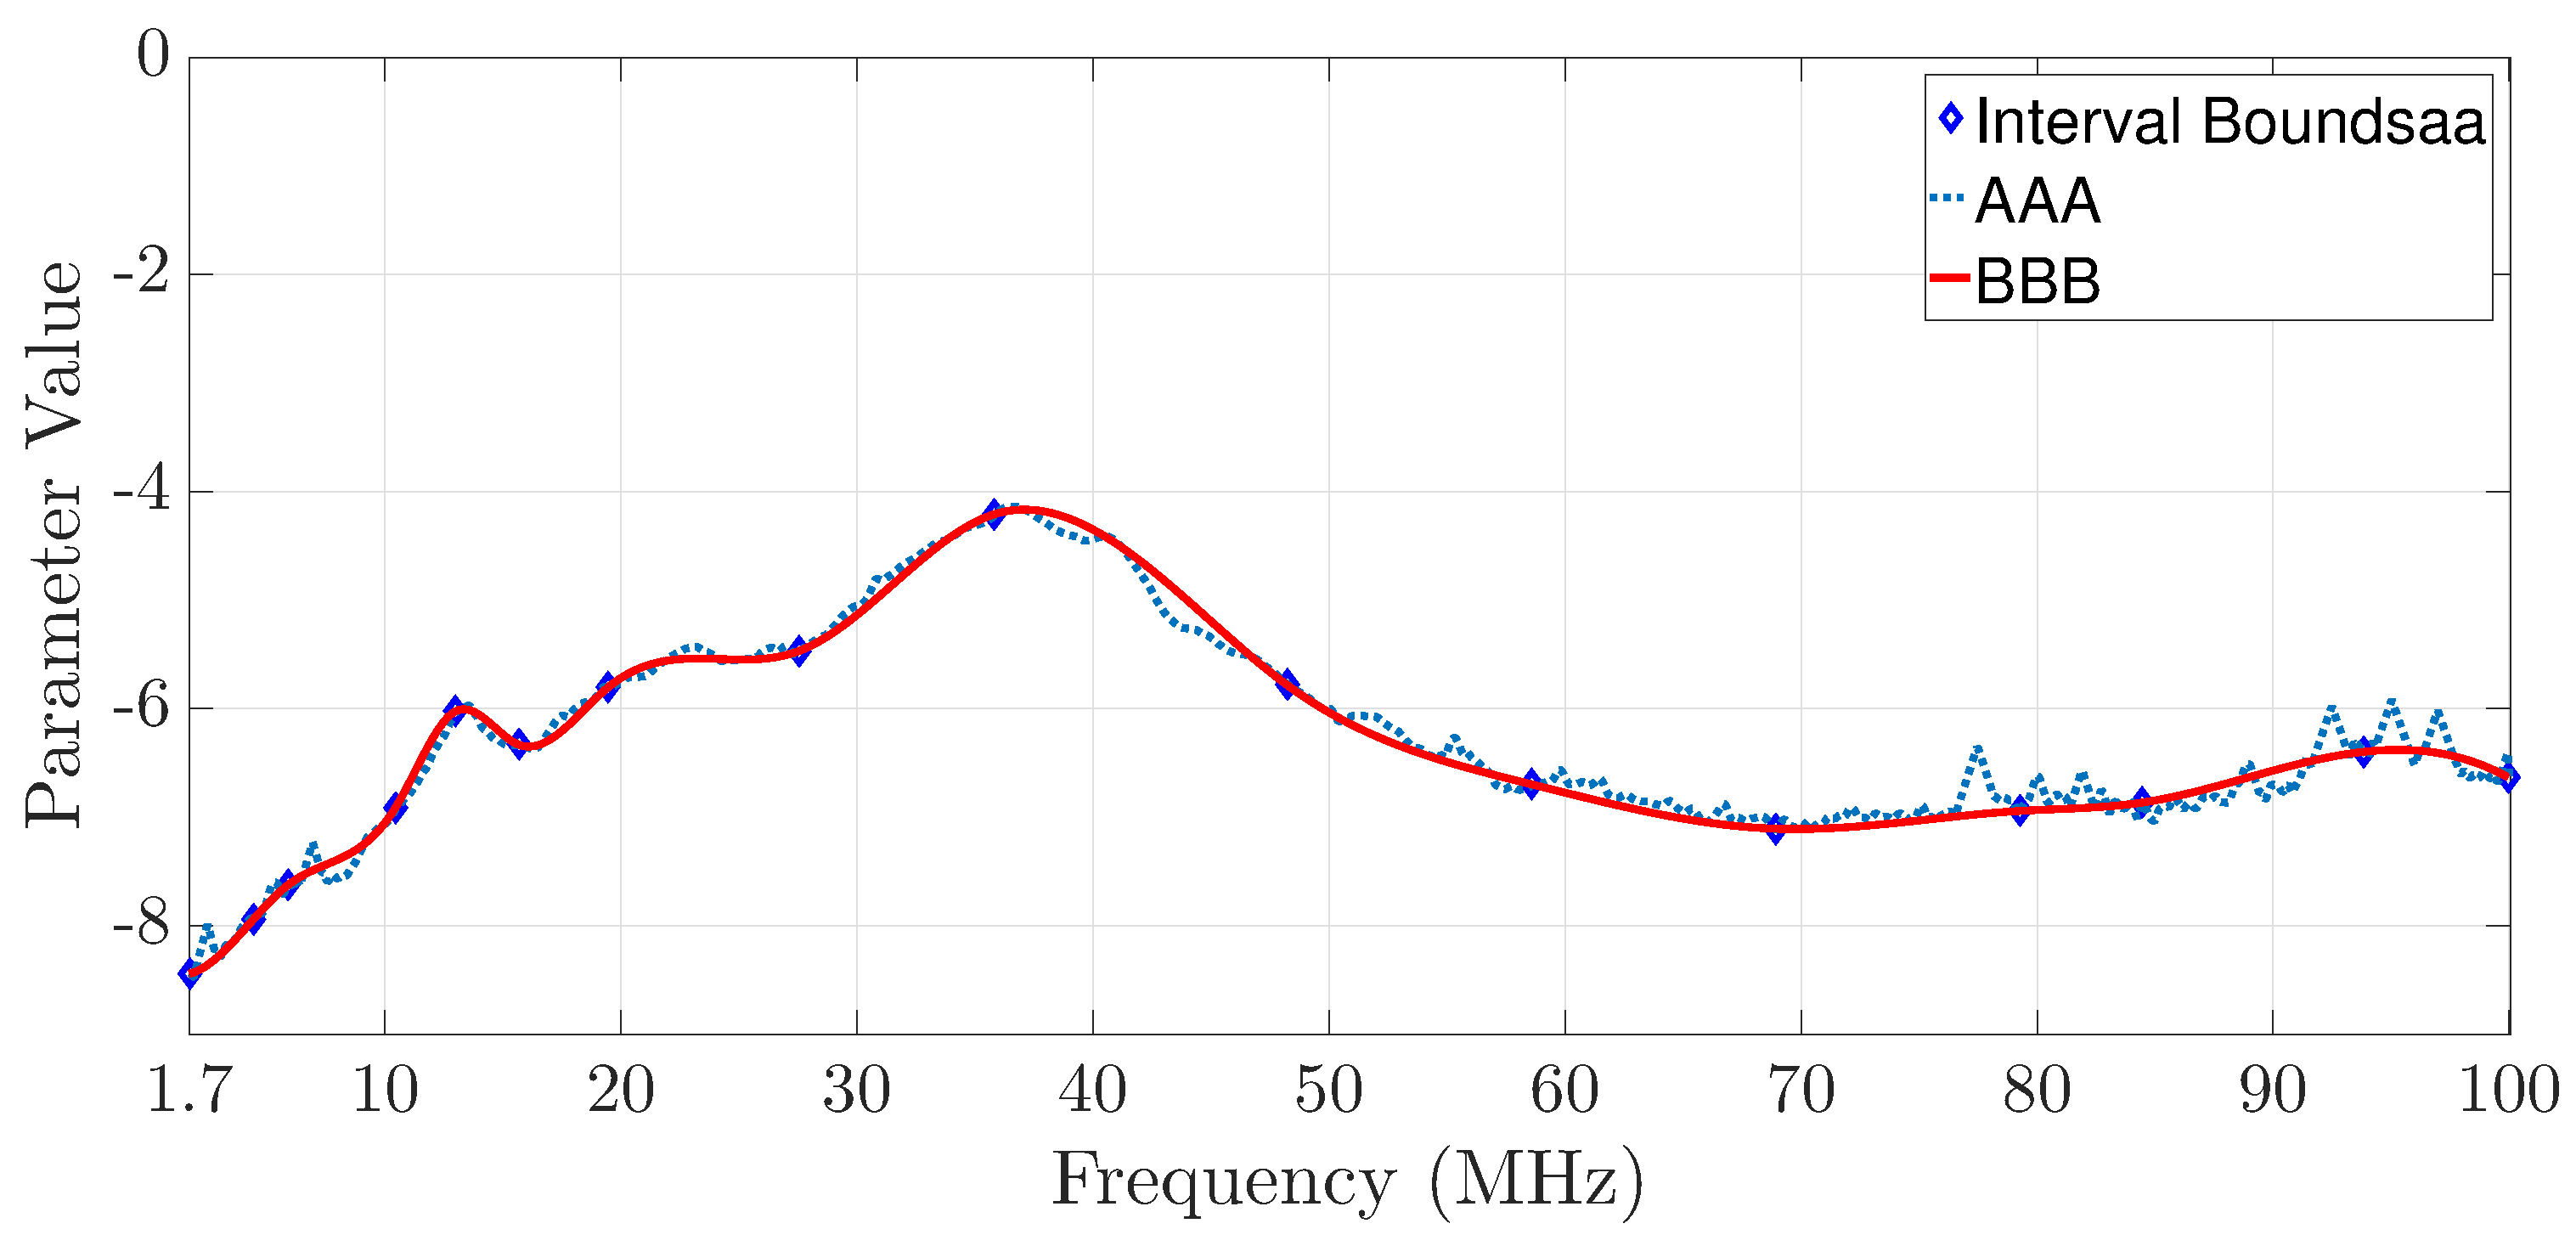
\includegraphics[width=0.49\textwidth]{images/Alfa_fitlW.eps}
	\caption{The result of the interpolation technique based on cubic Splines applied to obtain $\mu(f)=\zeta_1(f)$ for the Log-normal distribution (${\mu}(k \Delta f)$ are the original values of the parameter and $\hat{\mu}(f)$ is the interpolated curve).}
	\label{Fit_alfalW}
\end{figure}

\begin{figure}[h]
	\centering
	\psfrag{Interval Boundsaa}[c][c][0.7]{Interval Bounds}
	\psfrag{AAA}[c][c][0.7]{$~~~~~{\sigma}(k \Delta f)$}
	\psfrag{BBB}[c][c][0.7]{$~\hat{\sigma}(f)$}
	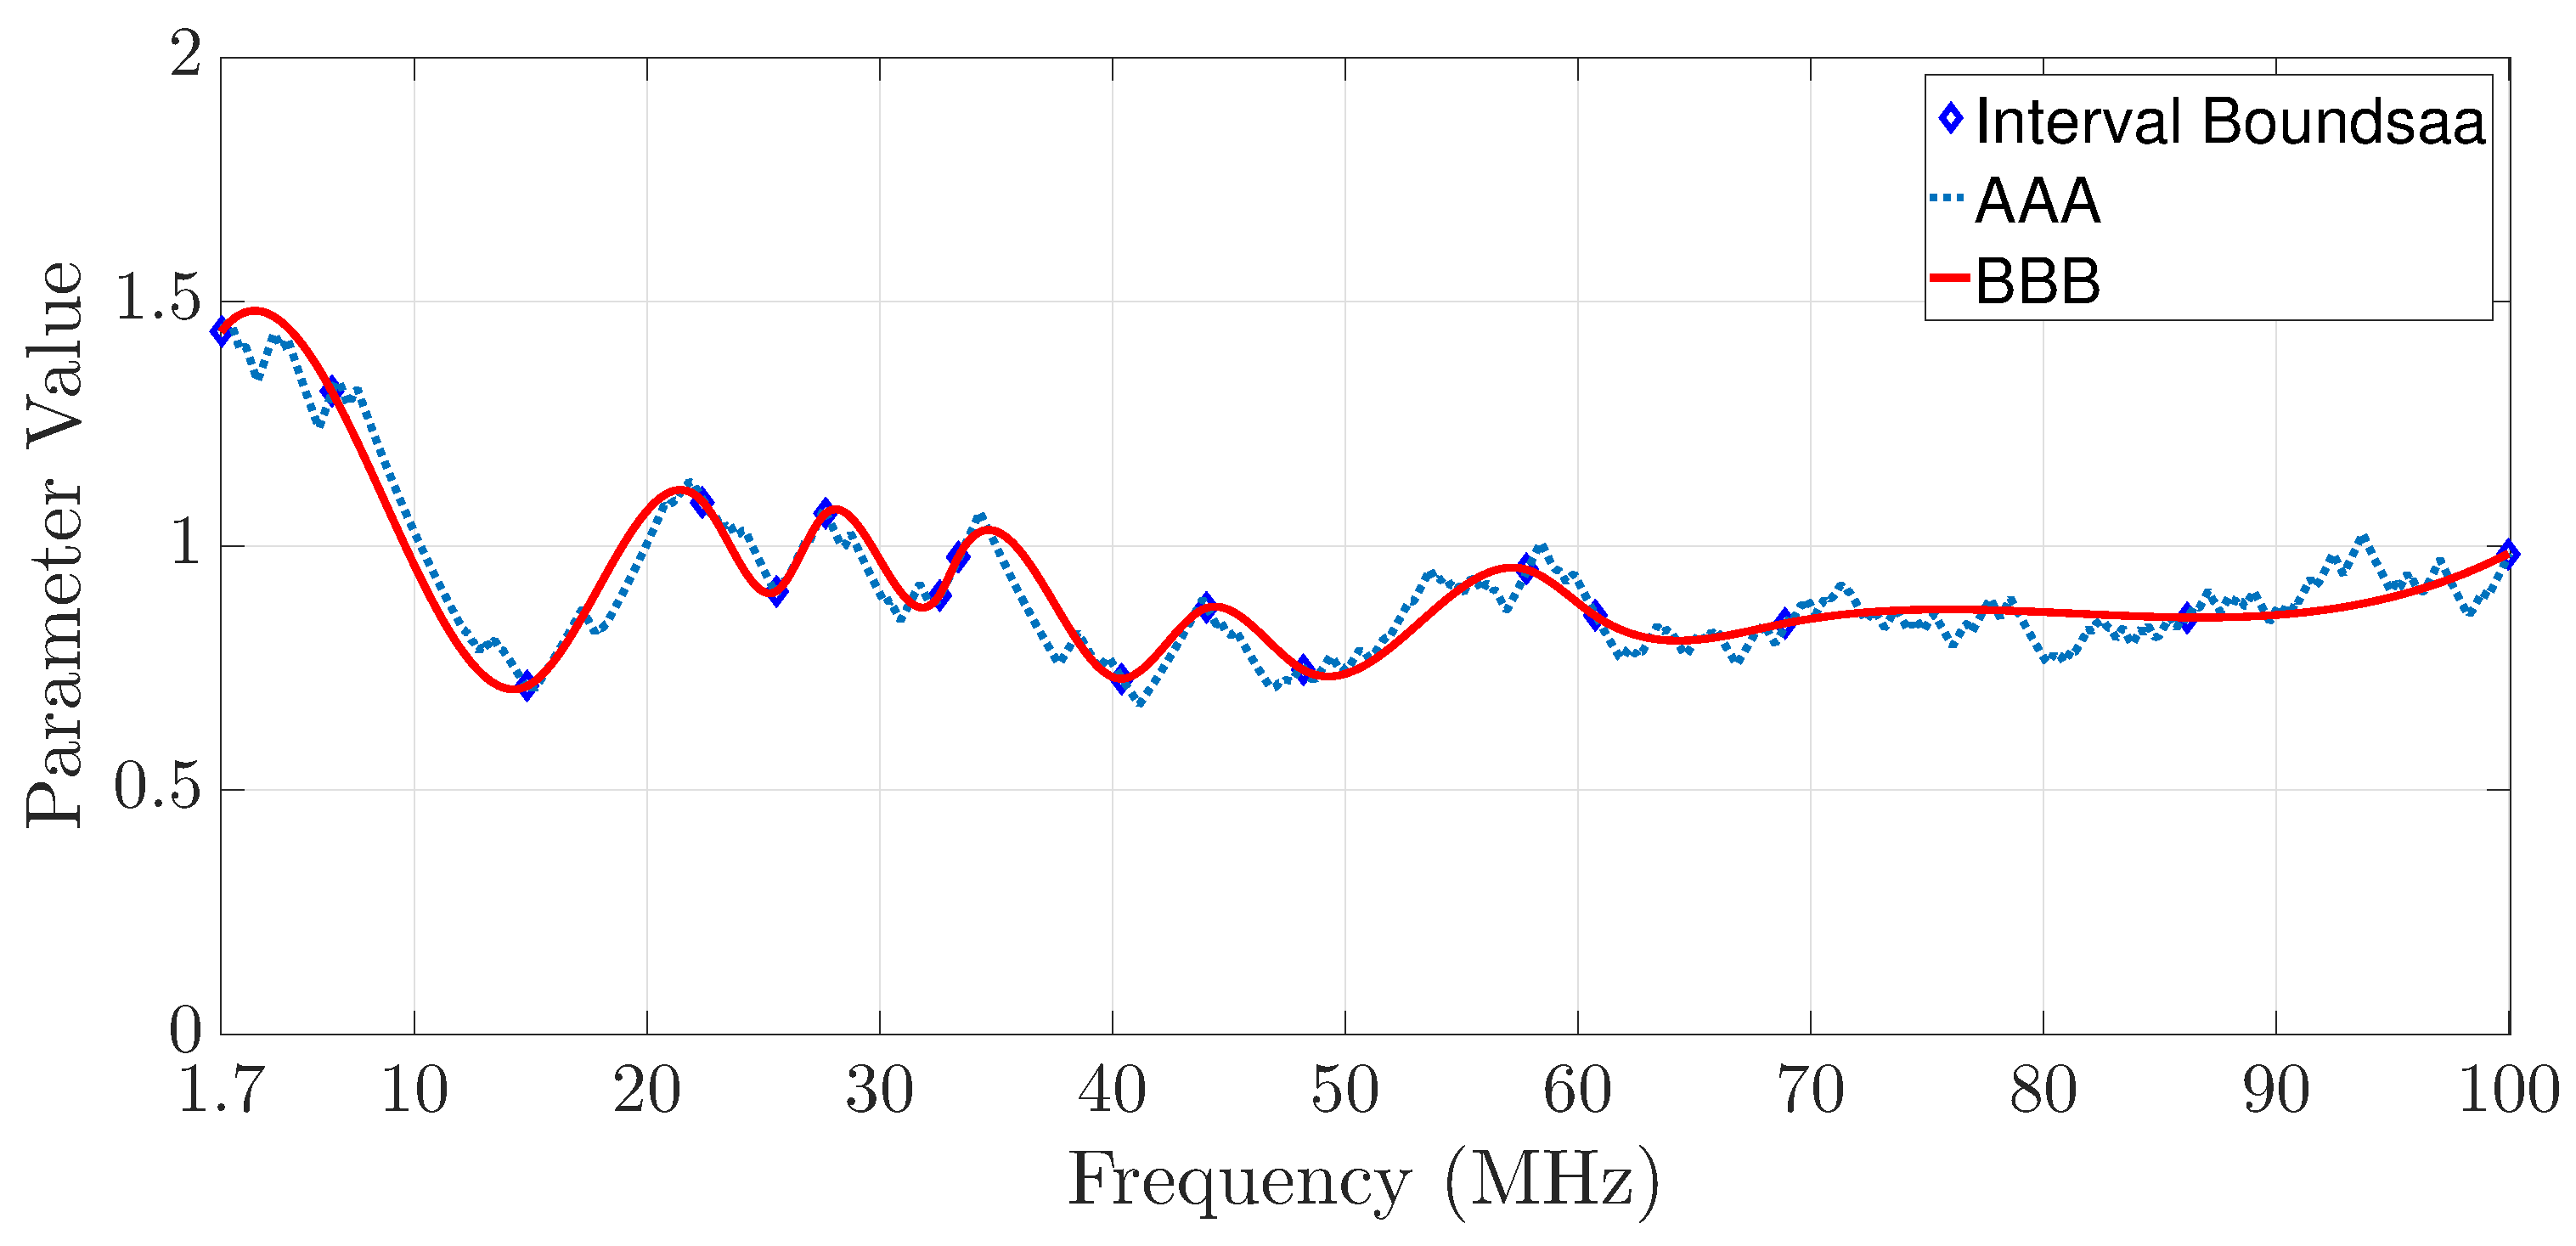
\includegraphics[width=0.49\textwidth]{images/Beta_fitlW.eps}
	\caption{The result of the interpolation technique based on cubic Splines applied to obtain $\sigma(f)=\zeta_2(f)$ for the Log-normal distribution (${\sigma}(k \Delta f)$ are the original values of the parameter and $\hat{\sigma}(f)$ is the interpolated curve).}
	\label{Fit_betalW}
\end{figure}

\section{Conclusions}
This paper has discussed statistical characterization and modeling of the \ac{CFR} magnitudes estimates of the Brazilian and broadband in-home \ac{PLC} and hybrid \ac{PLC}-\ac{WLC} channels, which constitutes an important issue to support research efforts for simulating and designing \ac{PLC} and hybrid \ac{PLC}-\ac{WLC} systems. The statistical characterization and modeling have been based on the analyses of data sets of measured \ac{CFR} estimates, covering the frequency band between $1.7$ and $100$~MHz. 

Numerical results have shown that the proposed method for modeling the magnitude of the aforementioned channels is suitable. Also, the magnitudes of the channel frequency responses of the broadband in-home \ac{PLC} and hybrid \ac{PLC}-\ac{WLC} channels are better modeled by Beta and Log-normal statistical distributions, respectively. Moreover, the results show that these magnitudes are non-stationary random processes. 
 
\section*{Acknowledgements}
Authors acknowledge financial support from CNPq, CAPES, FAPEMIG, Smarti9 LTD. and INERGE.

\bibliographystyle{IEEEtran}
\bibliography{Ref}

\begin{table*}[h]
	\setlength\extrarowheight{4.5pt}
	\centering
	\caption{$\alpha(f)$ parameter: Coefficients of the cubic Splines for the $L=19$ subintervals.}
	\label{table_alfa}
	\begin{tabular}{|C{4cm}|C{3cm}|C{3cm}|C{3cm}|C{3cm}|m{0cm}}
		\cline{1-5}
		Frequency Band (MHz)           		   & $a_u$    			  & $b_u$      			 & $c_u$   		 		& $d_u$&\\ \cline{1-5}
		$1.70\textless \mid f\mid \leq 3.42$   & -2.6528 $\times 10^{-5}$ & 0.0033  				 & -0.1197 					& 2.5007 &\\ \cline{1-5}
		$3.42\textless \mid f\mid \leq 4.44$   & -2.6528 $\times 10^{-5}$ & 5.2561 $\times 10^{-4}$  & 0.0146  					& 1.2292 &\\ \cline{1-5}
		$4.44\textless \mid f\mid \leq 6.05$   & 1.7869  $\times 10^{-5}$ & -0.0011                  & 0.0015                   & 1.5211 &\\ \cline{1-5}
		$6.05\textless \mid f\mid \leq 8.50$   & -5.9605 $\times 10^{-6}$ & 6.2337 $\times 10^{-4}$  & -0.0157                  & 0.9666 &\\ \cline{1-5}
		$8.50\textless \mid f\mid \leq 12.01$  & 2.0887  $\times 10^{-6}$ & -2.7071 $\times 10^{-4}$ & 0.0019 					& 0.9954 &\\ \cline{1-5}
		$12.01\textless \mid f\mid \leq 17.19$ & -9.2474 $\times 10^{-7}$ & 1.8046 $\times 10^{-4}$  & -0.0046 					& 0.5114 &\\ \cline{1-5}
		$17.19\textless \mid f\mid \leq 22.36$ & 6.4104  $\times 10^{-7}$ & -1.1361 $\times 10^{-4}$ & 0.0025  					& 0.9547 &\\ \cline{1-5}
		$22.36\textless \mid f\mid \leq 27.53$ & -5.6131 $\times 10^{-7}$ & 9.0243 $\times 10^{-5}$  & 5.3515 $\times 10^{-5}$  & 0.7099 &\\ \cline{1-5}
		$27.53\textless \mid f\mid \leq 32.71$ & 4.7371  $\times 10^{-7}$ & -8.8254 $\times 10^{-5}$ & -2.6432 $\times 10^{-4}$ & 1.0610 &\\ \cline{1-5}
		$32.71\textless \mid f\mid \leq 43.06$ & -1.7026 $\times 10^{-7}$ & 6.2385 $\times 10^{-5}$  & -0.0025 					& 0.6616 &\\ \cline{1-5}
		$43.06\textless \mid f\mid \leq 48.24$ & 1.4089  $\times 10^{-7}$ & -4.5902 $\times 10^{-5}$ & 0.0010  					& 1.3178 &\\ \cline{1-5}
		$48.24\textless \mid f\mid \leq 53.42$ & 1.4415  $\times 10^{-7}$ & -1.0984 $\times 10^{-6}$ & -0.0040 					& 1.0777 &\\ \cline{1-5}
		$53.42\textless \mid f\mid \leq 58.60$ & -2.7951 $\times 10^{-7}$ & 4.4742 $\times 10^{-5}$  & 6.6073 $\times 10^{-4}$  & 0.8167 &\\ \cline{1-5}
		$58.60\textless \mid f\mid \leq 68.95$ & 1.4642  $\times 10^{-7}$ & -4.4142 $\times 10^{-5}$ & 7.2426 $\times 10^{-4}$  & 1.0565 &\\ \cline{1-5}
		$68.95\textless \mid f\mid \leq 74.12$ & -3.5410 $\times 10^{-7}$ & 4.8981 $\times 10^{-5}$  & 0.0018 					& 0.6212 &\\ \cline{1-5}
		$74.12\textless \mid f\mid \leq 79.30$ & 4.3096  $\times 10^{-7}$ & -6.3623 $\times 10^{-5}$ & 1.9804 $\times 10^{-4}$  & 0.9354 &\\ \cline{1-5}
		$79.30\textless \mid f\mid \leq 84.47$ & -3.8389 $\times 10^{-7}$ & 7.3423 $\times 10^{-5}$  & 0.0012					& 0.7548 &\\ \cline{1-5}
		$84.47\textless \mid f\mid \leq 94.82$ & 9.4613 $\times 10^{-8}$  & -4.8652 $\times 10^{-5}$ & 0.0039 					& 1.2537 &\\ \cline{1-5}
		$94.82\textless \mid f\mid \leq 100$   & 9.4613  $\times 10^{-8}$ & 1.1522 $\times 10^{-5}$  & -0.0040					& 0.7874 &\\ \cline{1-5}
	\end{tabular}
\end{table*}

\begin{table*}[h!]
	\setlength\extrarowheight{4.5pt}
	\centering
	\caption{$\beta(f)$ parameter: Coefficients of the cubic Splines for the $L=19$ subintervals.}
	\label{table_beta}
	\begin{tabular}{|C{4cm}|C{3cm}|C{3cm}|C{3cm}|C{3cm}|m{0cm}}
		\cline{1-5}
		Frequency Band (MHz)           		   & $a_u$    			   & $b_u$      			  & $c_u$   		 		& $d_u$ &\\ \cline{1-5}
		$1.70\textless \mid f\mid \leq 3.42$   & 0 						   & 0.0112 				  & -0.3463 				& 5.1804  &\\ \cline{1-5}
		$3.42\textless \mid f\mid \leq 4.44$   & -9.0897 $\times 10^{-5}$  & 0.0016 				  & 0.1020  				& 2.8535  &\\ \cline{1-5}
		$4.44\textless \mid f\mid \leq 6.05$   & 6.0160  $\times 10^{-5}$  & -0.0041 				  & 0.0503 					& 4.8733  &\\ \cline{1-5}
		$6.05\textless \mid f\mid \leq 8.50$   & -1.9159 $\times 10^{-5}$  & 0.0019 				  & -0.0234 				& 4.2359  &\\ \cline{1-5}
		$8.50\textless \mid f\mid \leq 12.01$  & 7.2688  $\times 10^{-6}$  & -0.0010 				  & 0.0191 					& 5.3245  &\\ \cline{1-5}
		$12.01\textless \mid f\mid \leq 17.19$ & -3.1854 $\times 10^{-6}$  & 5.5773 $\times 10^{-4}$  & -0.0137 				& 4.1615  &\\ \cline{1-5}
		$17.19\textless \mid f\mid \leq 22.36$ & 3.4012 $\times 10^{-6}$   & -4.5522 $\times 10^{-4}$ & -0.0028  				& 5.1844  &\\ \cline{1-5}
		$22.36\textless \mid f\mid \leq 27.53$ & -3.4336 $\times 10^{-6}$  & 6.2635 $\times 10^{-4}$  & 0.0153 					& 3.8223  &\\ \cline{1-5}
		$27.53\textless \mid f\mid \leq 32.71$ & 1.8876  $\times 10^{-6}$  & -4.6554 $\times 10^{-4}$ & 0.0324 					& 8.3953  &\\ \cline{1-5}
		$32.71\textless \mid f\mid \leq 43.06$ & -2.0279 $\times 10^{-7}$  & 1.3472 $\times 10^{-4}$  & -0.0027 				& 8.8443  &\\ \cline{1-5}
		$43.06\textless \mid f\mid \leq 48.24$ & -1.1405  $\times 10^{-6}$ & 5.7440 $\times 10^{-6}$  & 0.0271  				& 12.3956 &\\ \cline{1-5}
		$48.24\textless \mid f\mid \leq 53.42$ & 2.6168  $\times 10^{-6}$  & -3.5693 $\times 10^{-4}$ & -0101 					& 13.9729 &\\ \cline{1-5}
		$53.42\textless \mid f\mid \leq 58.60$ & -2.6679 $\times 10^{-6}$  & 4.7522 $\times 10^{-4}$  & 0.0024 					& 12.0045 &\\ \cline{1-5}
		$58.60\textless \mid f\mid \leq 68.95$ & 1.4275  $\times 10^{-6}$  & -3.7318 $\times 10^{-4}$ & 0.0132 					& 14.4208 &\\ \cline{1-5}
		$68.95\textless \mid f\mid \leq 74.12$ & -4.7854 $\times 10^{-6}$  & 5.3473 $\times 10^{-4}$  & 0.0475 					& 14.0510 &\\ \cline{1-5}
		$74.12\textless \mid f\mid \leq 79.30$ & 8.4579  $\times 10^{-6}$  & -9.8702 $\times 10^{-4}$ & -4.8272 $\times 10^{-4}$& 19.3107 &\\ \cline{1-5}
		$79.30\textless \mid f\mid \leq 84.47$ & -9.4143 $\times 10^{-6}$  & 0.0017 				  & 0.0754 					& 18.3228 &\\ \cline{1-5}
		$84.47\textless \mid f\mid \leq 94.82$ & 3.5082 $\times 10^{-6}$   & -0.0013 				  & 0.1190					& 34.2297 &\\ \cline{1-5}
		$94.82\textless \mid f\mid \leq 100$   & 3.5082 $\times 10^{-6}$   & 9.4005 $\times 10^{-4}$  & 0.0445 					& 34.8507 &\\ \cline{1-5}
	\end{tabular}
\end{table*}

\begin{table*}[h]
	\setlength\extrarowheight{4.5pt}
	\centering
	\caption{$\mu(f)$ parameter: Coefficients of the cubic Splines for  $L=15$  nonuniform subbands.}
	\label{table_alfasW}
	\begin{tabular}{|C{4cm}|C{3cm}|C{3cm}|C{3cm}|C{3cm}|m{0cm}}
		\cline{1-5}
		Frequency Band (MHz)           		   & $a_u$    			  	  & $b_u$	      			  & $c_u$  	 		 		 & $d_u$&\\ \cline{1-5}
		$1.70\textless \mid f\mid \leq 5.08$   & 2.3701  $\times 10^{-6}$ & -6.0903 $\times 10^{-4}$  & 0.0500 					 & -7.9514 &\\ \cline{1-5}
		$5.08\textless \mid f\mid \leq 6.54$   & 2.3701  $\times 10^{-6}$ & -1.1842 $\times 10^{-4}$  & -1.7145 $\times 10^{-4}$ & -6.6209 &\\ \cline{1-5}
		$6.54\textless \mid f\mid \leq 8.50$   & 3.9289  $\times 10^{-6}$ & 9.4894  $\times 10^{-5}$  & -8.7708 $\times 10^{-4}$ & -6.6686 &\\ \cline{1-5}
		$8.50\textless \mid f\mid \leq 9.47$   & -1.7588 $\times 10^{-5}$ & 5.6636  $\times 10^{-4}$  & 0.0256                   & -6.3004 &\\ \cline{1-5}
		$9.47\textless \mid f\mid \leq 13.87$  & 2.4037  $\times 10^{-6}$ & -4.8890 $\times 10^{-4}$  & 0.0271					 & -5.7031 &\\ \cline{1-5}
		$13.87\textless \mid f\mid \leq 21.19$ & -5.6687 $\times 10^{-7}$ & 1.6009  $\times 10^{-4}$  & -0.0025		    		 & -5.4699 &\\ \cline{1-5}
		$21.19\textless \mid f\mid \leq 28.03$ & 3.7473  $\times 10^{-7}$ & -9.4996 $\times 10^{-5}$  & 0.0073  				 & -4.1516 &\\ \cline{1-5}
		$28.03\textless \mid f\mid \leq 33.40$ & -3.4080 $\times 10^{-7}$ & 6.2389  $\times 10^{-5}$  & 0.0027 					 & -3.9641 &\\ \cline{1-5}
		$33.40\textless \mid f\mid \leq 43.46$ & 1.0904  $\times 10^{-7}$ & -5.0076 $\times 10^{-5}$  & 0.0041  				 & -3.3626 &\\ \cline{1-5}
		$43.46\textless \mid f\mid \leq 50.49$ & -8.8509 $\times 10^{-8}$ & 1.7312  $\times 10^{-5}$  & -0.0027					 & -3.6932 &\\ \cline{1-5}
		$50.49\textless \mid f\mid \leq 55.37$ & 1.2130  $\times 10^{-7}$ & -2.0924 $\times 10^{-5}$  & -0.0032  				 & -3.9824 &\\ \cline{1-5}
		$55.37\textless \mid f\mid \leq 65.14$ & -3.1804 $\times 10^{-8}$ & 1.5465  $\times 10^{-5}$  & -0.0037 				 & -4.3889 &\\ \cline{1-5}
		$65.14\textless \mid f\mid \leq 74.90$ & 1.7372  $\times 10^{-8}$ & -3.6169 $\times 10^{-6}$  & -0.0014  			     & -4.7710 &\\ \cline{1-5}
		$74.90\textless \mid f\mid \leq 96.87$ & -1.2395 $\times 10^{-8}$ & 6.8061  $\times 10^{-6}$  & -7.2408 $\times 10^{-4}$ & -5.0491 &\\ \cline{1-5}
		$96.87\textless \mid f\mid \leq 100$   & -1.2395 $\times 10^{-8}$ & -9.9272 $\times 10^{-6}$  & -0.0021 				 & -5.1262 &\\ \cline{1-5}
	\end{tabular}
\end{table*}

\begin{table*}[h]
	\setlength\extrarowheight{4.5pt}
	\centering
	\caption{$\sigma(f)$ parameter: Coefficients of the cubic Splines for the $L=15$ nonuniform subbands.}
	\label{table_betasW}
	\begin{tabular}{|C{4cm}|C{3cm}|C{3cm}|C{3cm}|C{3cm}|m{0cm}}
		\cline{1-5}
		Frequency Band (MHz)           		   & $a_u$    			   	   & $b_u$      			  & $c_u$   		 		 & $d_u$ &\\ \cline{1-5}
		$1.70\textless \mid f\mid \leq 2.88$   & 2.1232 $\times 10^{-5}$   & -0.0021 				  & 0.0435	 				 & 1.2187 &\\ \cline{1-5}
		$2.88\textless \mid f\mid \leq 4.35$   & 2.1232 $\times 10^{-5}$   & -5.2494 $\times 10^{-4}$ & -0.0184  				 & 1.3724 &\\ \cline{1-5}
		$4.35\textless \mid f\mid \leq 5.08$   & -5.8155 $\times 10^{-5}$  & 0.0014 				  & 0.0074 					 & 0.9206 &\\ \cline{1-5}
		$5.08\textless \mid f\mid \leq 6.54$   & 2.0568 $\times 10^{-5}$   & -0.0012 				  & 0.0097	 				 & 1.1473 &\\ \cline{1-5}
		$6.54\textless \mid f\mid \leq 8.50$   & -8.0700 $\times 10^{-6}$  & 6.2010 $\times 10^{-4}$  & -0.0086 				 & 0.8867 &\\ \cline{1-5}
		$8.50\textless \mid f\mid \leq 10.69$  & 3.7423 $\times 10^{-6}$   & -3.4830 $\times 10^{-4}$ & 0.0023	 				 & 1.0186 &\\ \cline{1-5}
		$10.69\textless \mid f\mid \leq 17.28$ & -6.3590 $\times 10^{-7}$  & 1.5692 $\times 10^{-4}$  & -0.0063  				 & 0.7568 &\\ \cline{1-5}
		$17.28\textless \mid f\mid \leq 22.66$ & 4.4496 $\times 10^{-7}$   & -1.0063 $\times 10^{-4}$ & 0.0013 					 & 1.1968 &\\ \cline{1-5}
		$22.66\textless \mid f\mid \leq 35.06$ & -1.0044  $\times 10^{-7}$ & 4.6212 $\times 10^{-5}$  & -0.0047					 & 0.7106 &\\ \cline{1-5}
		$35.06\textless \mid f\mid \leq 39.84$ & 1.5003  $\times 10^{-7}$  & -3.0325 $\times 10^{-5}$ & -6.8556 $\times 10^{-4}$ & 0.8469 &\\ \cline{1-5}
		$39.84\textless \mid f\mid \leq 60.25$ & -1.8796 $\times 10^{-8}$  & 1.3785  $\times 10^{-5}$ & -0.0023  				 & 0.6297 &\\ \cline{1-5}
		$60.25\textless \mid f\mid \leq 68.55$ & 1.2989   $\times 10^{-7}$ & -9.7855 $\times 10^{-6}$ & -6.3475	$\times 10^{-4}$ & 0.7014 &\\ \cline{1-5}
		$78.61\textless \mid f\mid \leq 78.61$ & -2.1013 $\times 10^{-7}$  & 2.9181  $\times 10^{-5}$ & 0.0013					 & 0.6699 &\\ \cline{1-5}
		$78.61\textless \mid f\mid \leq 94.43$ & 2.2893  $\times 10^{-8}$  & -1.4947 $\times 10^{-5}$ & 0.0023				     & 0.8322 &\\ \cline{1-5}
		$94.43\textless \mid f\mid \leq 100$   & 1.0785  $\times 10^{-8}$  & -5.2390 $\times 10^{-7}$ & -9.4771 $\times 10^{-4}$ & 0.8683 &\\ \cline{1-5}
	\end{tabular}
\end{table*}

\begin{table*}[h]
	\setlength\extrarowheight{4.5pt}
	\centering
	\caption{$\mu(f)$ parameter: Coefficients of the cubic Splines for $L=15$ nonuniform subbands.}
	\label{table_alfalW}
	\begin{tabular}{|C{4cm}|C{2.7cm}|C{2.7cm}|C{2.7cm}|C{2.7cm}|m{0cm}}
		\cline{1-5}
		Frequency Band (MHz)           		   & $a_u$    			   	   & $b_u$      			  & $c_u$   		 		 & $d_u$ &\\ \cline{1-5}
		$1.70\textless \mid f\mid \leq 6.44$   & -1.1271 $\times 10^{-6}$  & 1.7728 $\times 10^{-4}$  & 0.0026	 				 & -8.4445 &\\ \cline{1-5}
		$6.44\textless \mid f\mid \leq 14.84$  & -1.1271 $\times 10^{-6}$  & -1.2068 $\times 10^{-5}$ & 0.0119  				 & -7.9388 &\\ \cline{1-5}
		$14.84\textless \mid f\mid \leq 22.41$ & 1.1653  $\times 10^{-6}$  & -1.1350 $\times 10^{-4}$ & 0.0081 					 & -7.6235 &\\ \cline{1-5}
		$22.41\textless \mid f\mid \leq 25.59$ & -4.1434 $\times 10^{-6}$  & 2.1163 $\times 10^{-4}$  & 0.0172	 				 & -6.9126 &\\ \cline{1-5}
		$25.59\textless \mid f\mid \leq 27.69$ & 4.1926 $\times 10^{-6}$   & -4.3475 $\times 10^{-4}$ & 0.0056					 & -6.0262 &\\ \cline{1-5}
		$27.69\textless \mid f\mid \leq 32.57$ & -1.4955 $\times 10^{-6}$  & 2.5704 $\times 10^{-4}$  & -0.0041	 				 & -6.3333 &\\ \cline{1-5}
		$32.57\textless \mid f\mid \leq 33.40$ & 3.1809 $\times 10^{-7}$   & -9.2908 $\times 10^{-5}$ & 0.0087   				 & -5.8014 &\\ \cline{1-5}
		$33.40\textless \mid f\mid \leq 40.38$ & -2.6103 $\times 10^{-7}$  & 6.4547 $\times 10^{-5}$  & 0.0040 					 & -5.4711 &\\ \cline{1-5}
		$40.38\textless \mid f\mid \leq 44.04$ & 1.2268  $\times 10^{-7}$  & -6.8577 $\times 10^{-5}$ & 0.0033					 & -4.2094 &\\ \cline{1-5}
		$44.04\textless \mid f\mid \leq 48.24$ & -4.0204 $\times 10^{-8}$  & 2.4906 $\times 10^{-5}$  & -0.0078	 				 & -5.7833 &\\ \cline{1-5}
		$48.24\textless \mid f\mid \leq 57.81$ & 1.8952  $\times 10^{-8}$  & -6.6395 $\times 10^{-7}$ & -0.0026  				 & -6.6975 &\\ \cline{1-5}
		$57.81\textless \mid f\mid \leq 60.74$ & -2.8253  $\times 10^{-8}$ & 1.1389 $\times 10^{-5}$  & -3.7214 $\times 10^{-4}$ & -7.1077 &\\ \cline{1-5}
		$60.74\textless \mid f\mid \leq 68.94$ & 6.8867 $\times 10^{-8}$   & -6.5792 $\times 10^{-6}$ & 6.4762	$\times 10^{-4}$ & -6.9439 &\\ \cline{1-5}
		$68.94\textless \mid f\mid \leq 86.18$ & -5.6494  $\times 10^{-8}$ & 1.5321 $\times 10^{-5}$  & 0.0016 				     & -6.8672 &\\ \cline{1-5}
		$86.18\textless \mid f\mid \leq 100$   & -5.6494 $\times 10^{-8}$  & -1.7390 $\times 10^{-5}$ & 0.0012  				 & -6.3988 &\\ \cline{1-5}
	\end{tabular}
\end{table*}

\begin{table*}[h]
	\setlength\extrarowheight{4.5pt}
	\centering
	\caption{$\sigma(f)$ parameter: Coefficients of the cubic Splines for the $L=15$ nonuniform subbands.}
	\label{table_betalW}
	\begin{tabular}{|C{4cm}|C{2.7cm}|C{2.7cm}|C{2.7cm}|C{2.7cm}|m{0cm}}
		\cline{1-5}
		Frequency Band (MHz)           		   & $a_u$    			   	   & $b_u$      			  & $c_u$   		 		 & $d_u$ &\\ \cline{1-5}
		$1.70\textless \mid f\mid \leq 4.44$   & 1.3148  $\times 10^{-7}$  & -5.6568 $\times 10^{-5}$ & 0.0030	 				 & 1.4384 &\\ \cline{1-5}
		$4.44\textless \mid f\mid \leq 5.91$   & 1.3148  $\times 10^{-7}$  & -1.8306 $\times 10^{-5}$ & -0.0043  				 & 1.3175 &\\ \cline{1-5}
		$5.91\textless \mid f\mid \leq 10.45$  & -2.6464 $\times 10^{-7}$  & 4.9539 $\times 10^{-5}$  & 0.0011					 & 0.7124 &\\ \cline{1-5}
		$10.45\textless \mid f\mid \leq 12.99$ & 1.0831  $\times 10^{-6}$  & -7.3521 $\times 10^{-5}$ & -0.0026	 				 & 1.0896 &\\ \cline{1-5}
		$12.99\textless \mid f\mid \leq 15.68$ & -2.0515 $\times 10^{-6}$  & 1.3768  $\times 10^{-4}$ & 0.0016  				 & 0.9071 &\\ \cline{1-5}
		$15.68\textless \mid f\mid \leq 19.48$ & 8.9917 $\times 10^{-7}$   & -1.2695 $\times 10^{-4}$ & 0.0020	 				 & 1.0660 &\\ \cline{1-5}
		$19.48\textless \mid f\mid \leq 27.54$ & -4.7172 $\times 10^{-6}$  & 1.4280 $\times 10^{-4}$  & 0.0036 					 & 0.8984 &\\ \cline{1-5}
		$27.54\textless \mid f\mid \leq 35.84$ & 3.8415  $\times 10^{-7}$  & -9.7780 $\times 10^{-5}$ & 0.0044 					 & 0.9779 &\\ \cline{1-5}
		$35.84\textless \mid f\mid \leq 48.24$ & -5.4667 $\times 10^{-7}$  & 6.7022 $\times 10^{-5}$  & -2.1365	$\times 10^{-5}$ & 0.7276 &\\ \cline{1-5}
		$48.24\textless \mid f\mid \leq 58.59$ & 3.4176  $\times 10^{-7}$  & -5.5979 $\times 10^{-5}$ & 8.0683	$\times 10^{-4}$ & 0.8724 &\\ \cline{1-5}
		$58.59\textless \mid f\mid \leq 68.94$ & -1.0467 $\times 10^{-7}$  & 3.2196 $\times 10^{-5}$  & -0.0012  				 & 0.7451 &\\ \cline{1-5}
		$68.94\textless \mid f\mid \leq 79.30$ & 2.4291  $\times 10^{-7}$  & -2.9349 $\times 10^{-5}$ & -6.8042	$\times 10^{-4}$ & 0.9511 &\\ \cline{1-5}
		$79.30\textless \mid f\mid \leq 84.47$ & -3.2976 $\times 10^{-8}$  & 1.4375 $\times 10^{-5}$  & -0.0016  				 & 0.8571 &\\ \cline{1-5}
		$84.47\textless \mid f\mid \leq 93.90$ & 2.9498  $\times 10^{-9}$  & -2.2454 $\times 10^{-6}$ & 4.5886	$\times 10^{-4}$ & 0.8412 &\\ \cline{1-5}
		$93.90\textless \mid f\mid \leq 100$   & 2.9498  $\times 10^{-9}$  & 8.7842 $\times 10^{-7}$  & -2.3694 $\times 10^{-5}$ & 0.8531 &\\ \cline{1-5}
	\end{tabular}
\end{table*}

\end{document}